% Preambel mit Einstellungen importieren
% Document type and used packages
\documentclass[open=right, % Sorgt für Umbruch bei Chapter (any erzeugt keine Leerseiten) -> Kapitel darf nur auf der rechten Seite beginnen
    paper=A4,               % DIN-A4-Papier
    a4paper,                % DIN-A4-Papier
    12pt,                   % Schriftgöße
    headings=small,         % Kleine Überschriften
    headsepline=true,       % Trennlinie am Kopf der Seite
    footsepline=false,      % Keine Trennlinie am Fuß der Seite
    bibliography=totoc,     % Literaturverzeichnis in das Inhaltsverzeichnis aufnehmen
    twoside=on,             % Doppelseitiger Druck - auf off stellen für einseitig
    DIV=7,                  % Verhältnis der Ränder zum bedruckten Bereich
    chapterprefix=false,     % Kapitel x vor dem Kapitelnamen
    cleardoublepage=plain]{scrbook}


\usepackage{morewrites}

% Pakete einbinden, die benötigt werden
\usepackage{scrpage2}
\usepackage[utf8]{inputenc}       % Dateien in UTF-8 benutzen
\usepackage[T1]{fontenc}          % Zeichenkodierung
\usepackage{graphicx}             % Bilder einbinden
\usepackage[main=ngerman, english]{babel}       % Deutsch und Englisch unterstützen
\usepackage{xcolor}               % Color support
\usepackage{amsmath}              % Matheamtische Formeln
\usepackage{amsfonts}             % Mathematische Zeichensätze
\usepackage{amssymb}              % Mathematische Symbole
\usepackage{float}                % Fließende Objekte (Tabellen, Grafiken etc.)
\usepackage{booktabs}             % Korrekter Tabellensatz
\usepackage[printonlyused, withpage, footnote]{acronym}  % Abkürzungsverzeichnis [nur verwendete Abkürzugen]
\usepackage{makeidx}              % Sachregister
\usepackage{listings}             % Source Code listings
\usepackage{listingsutf8}         % Listings in UTF8
\usepackage[hang,font={sf,footnotesize},labelfont={footnotesize,bf}]{caption} % Beschriftungen
\usepackage[scaled]{helvet}       % Schrift Helvetia laden
\usepackage[absolute]{textpos}	  % Absolute Textpositionen (für Deckblatt)
\usepackage{calc}                 % Berechnung von Positionen
\usepackage{blindtext}            % Blindtexte
\usepackage[bottom=40mm,left=35mm,right=35mm,top=30mm]{geometry} % Ränder ändern
\usepackage{setspace}             % Abstände korrigieren
\usepackage{ifthen}               % Logische Bedingungen mit ifthenelse
\usepackage{scrhack}              % Get rid of tocbasic warnings
\usepackage[pagebackref=false,german]{hyperref}  % Hyperlinks
\usepackage[all]{hypcap}          % Korrekte Verlinkung von Floats
\usepackage[autostyle=true,german=quotes]{csquotes}   % Zitate
\usepackage[backend=biber,
  isbn=true,                     % ISBN nicht anzeigen, gleiches geht mit nahezu allen anderen Feldern
  sortlocale=de_DE,               % Sortierung der Einträge für Deutsch
  %sortlocale=en_US,              % Sortierung der Einträge für Englisch
  autocite=inline,                % regelt Aussehen für \autocite (inline=\parancite)
  hyperref=true,                  % Hyperlinks für Ziate
  %style=ieee                     % Zitate als Zahlen [1]
  %style=alphabetic               % Zitate als Kürzel und Jahr [Ein05]
  %style=authoryear                % Zitate Author und Jahr [Einstein (1905)]
  style=LNI
]{biblatex}                       % Literaturverwaltung mit BibLaTeX
\usepackage{rotating}             % Seiten drehen
\usepackage{harveyballs}          % Harveyballs
\usepackage{tcolorbox}
\usepackage[export]{adjustbox}
\usepackage{subcaption}
\usepackage{color}
\usepackage{colortbl}
\usepackage{wrapfig}
\usepackage{todonotes}
\usepackage{tabularx}
\newcolumntype{b}{>{\hsize=1.2\hsize}X}
\newcolumntype{m}{>{\hsize=.5\hsize}X}
\newcolumntype{s}{>{\hsize=.3\hsize}X}
\usepackage{tikz}


\setlength{\bibitemsep}{1em}     % Abstand zwischen den Literaturangaben
\setlength{\bibhang}{2em}        % Einzug nach jeweils erster Zeile

% Trennung von URLs im Literaturverzeichnis (große Werte [> 10000] verhindern die Trennung)
\defcounter{biburlnumpenalty}{10} % Strafe für Trennung in URL nach Zahl
\defcounter{biburlucpenalty}{500}  % Strafe für Trennung in URL nach Großbuchstaben
\defcounter{biburllcpenalty}{500}  % Strafe für Trennung in URL nach Kleinbuchstaben

% Farben definieren
\definecolor{linkblue}{RGB}{0, 0, 100}
\definecolor{linkblack}{RGB}{0, 0, 0}
\definecolor{comment}{RGB}{63, 127, 95}
\definecolor{darkgreen}{RGB}{14, 144, 102}
\definecolor{darkblue}{RGB}{0,0,168}
\definecolor{darkred}{RGB}{128,0,0}
\definecolor{javadoccomment}{RGB}{0,0,240}
\definecolor{Gray}{RGB}{242,242,242}

% Einstellungen für das Hyperlink-Paket
\hypersetup{
    colorlinks=true,      % Farbige links verwenden
%    allcolors=linkblue,
    linktoc=all,          % Links im Inhaltsverzeichnis
    linkcolor=linkblack,  % Querverweise
    citecolor=linkblack,  % Literaturangaben
	filecolor=linkblack,  % Dateilinks
	urlcolor=linkblack    % URLs
}

% Einstellungen für Quelltexte
\definecolor{backcolour}{rgb}{0.95,0.95,0.92}
\definecolor{codegray}{rgb}{0.5,0.5,0.5}
\lstset{
      xleftmargin=0.1cm,
      basicstyle=\footnotesize\ttfamily,
      keywordstyle=\color{darkgreen},
      identifierstyle=\color{darkblue},
      commentstyle=\color{comment},
      stringstyle=\color{darkred},
      tabsize=2,
      lineskip={2pt},
      columns=flexible,
      inputencoding=utf8,
      captionpos=b,
      backgroundcolor=\color{backcolour},   
      breakautoindent=true,
	  breakindent=2em,
	  breaklines=true,
	  prebreak=,
	  postbreak=,
      numbers=left,                    
      numbersep=5pt,  
      numberstyle=\tiny\color{codegray},  
      showspaces=false,      % Keine Leerzeichensymbole
      showtabs=false,        % Keine Tabsymbole
      showstringspaces=false,% Leerzeichen in Strings
      morecomment=[s][\color{javadoccomment}]{/**}{*/},
      literate={Ö}{{\"O}}1 {Ä}{{\"A}}1 {Ü}{{\"U}}1 {ß}{{\ss}}2 {ü}{{\"u}}1 {ä}{{\"a}}1 {ö}{{\"o}}1
}


\urlstyle{same}

% Einstellungen für Überschriften
\renewcommand*{\chapterformat}{%
  \Large~\thechapter. ~   		% Große Schrift
  \vspace{0.3cm}               	% Abstand zum Titel des Kapitels
}

% Abstände für die Überschriften setzen
\renewcommand{\chapterheadstartvskip}{\vspace*{2.6cm}}
\renewcommand{\chapterheadendvskip}{\vspace*{1.5cm}}

\RedeclareSectionCommand[
  beforeskip=-1.8\baselineskip,
  afterskip=0.25\baselineskip]{section}

\RedeclareSectionCommand[
  beforeskip=-1.8\baselineskip,
  afterskip=0.15\baselineskip]{subsection}

\RedeclareSectionCommand[
  beforeskip=-1.8\baselineskip,
  afterskip=0.15\baselineskip]{subsubsection}


% In der Kopfzeile nur die kurze Kapitelbezeichnung (ohne Kapitel davor)
\renewcommand*\chaptermarkformat{\thechapter\autodot\enskip}
\automark[chapter]{chapter}

% Einstellungen für Schriftarten
\setkomafont{pagehead}{\normalfont\sffamily}
\setkomafont{pagenumber}{\normalfont\sffamily}
\setkomafont{paragraph}{\sffamily\bfseries\small}
\setkomafont{subsubsection}{\sffamily\itshape\bfseries\small}
\addtokomafont{footnote}{\footnotesize}
\setkomafont{chapter}{\LARGE\selectfont\bfseries}

% Wichtige Abstände
\setlength{\parskip}{0.2cm}  % 2mm Abstand zwischen zwei Absätzen
\setlength{\parindent}{0mm}  % Absätze nicht einziehen
\clubpenalty = 10000         % Keine "Schusterjungen"
\widowpenalty = 10000        % Keine "Hurenkinder"
\displaywidowpenalty = 10000 % Keine "Hurenkinder"
\renewcommand{\footnotesize}{\fontsize{9}{10}\selectfont} % Größe der Fußnoten
\setlength{\footnotesep}{8pt} % Abstand zwischen den Fußnoten

% Index erzeugen
\makeindex

% Einfacher Font-Wechsel über dieses Makro
\newcommand{\changefont}[3]{
\fontfamily{#1} \fontseries{#2} \fontshape{#3} \selectfont}

% Eigenes Makro für Bilder
\newcommand{\bild}[3]{
\begin{figure}[h]
  \centering
  \includegraphics[width=#2]{#1}
  \caption{#3}
  \label{#1}
\end{figure}}

% Wo liegt Sourcecode?
\newcommand{\srcloc}{src/}

% Wo sind die Bilder?
\graphicspath{{bilder/}}

% Makros für typographisch korrekte Abkürzungen
\newcommand{\zb}[0]{z.\,B.\ }
\newcommand{\dahe}[0]{d.\,h.\ }
\newcommand{\ua}[0]{u.\,a.\ }

% Flags für Veröffentlichung und Sperrvermerk
\newboolean{hsmapublizieren}
\newboolean{hsmasperrvermerk}


% Dokumenteninfos importieren
% In docinfo.tex sind Titel, Autor, Abstract zu definieren
% -------------------------------------------------------
% Daten für die Arbeit
% Wenn hier alles korrekt eingetragen wurde, wird das Titelblatt
% automatisch generiert. D.h. die Datei titelblatt.tex muss nicht mehr
% angepasst werden.

\newcommand{\hsmasprache}{de} % de oder en für Deutsch oder Englisch
% Für korrekt sortierte Literatureinträge, noch preambel.tex anpassen
% und zwar bei \usepackage[main=ngerman, english]{babel},
% \usepackage[pagebackref=false,german]{hyperref}
% und \usepackage[autostyle=true,german=quotes]{csquotes}

% Titel der Arbeit auf Deutsch
\newcommand{\hsmatitelde}{Aufgabenfokussierung auf Autoencoder und automatisches Transferlernen}

% Titel der Arbeit auf Englisch
\newcommand{\hsmatitelen}{Task focusing on autoencoder and automatic transfer learning}

% Weitere Informationen zur Arbeit
\newcommand{\hsmaort}{Offenburg}    % Ort
\newcommand{\hsmaautorvname}{Sebastian} % Vorname(n)
\newcommand{\hsmaautornname}{Hoch} % Nachname(n)
\newcommand{\hsmadatum}{30 Juni 2020} % Datum der Abgabe
\newcommand{\hsmajahr}{2020} % Jahr der Abgabe
\newcommand{\hsmafirma}{PSIORI GmbH} % Firma bei der die Arbeit durchgeführt wurde
\newcommand{\hsmabetreuer}{Prof. Dr.-Ing. Janis Keuper, Hochschule Offenburg} % Betreuer an der Hochschule
\newcommand{\hsmazweitkorrektor}{Dr. rer. nat. Sascha Lange, PSIORI GmbH} % Betreuer im Unternehmen oder Zweitkorrektor
\newcommand{\hsmafakultaet}{EMI} % Fakultät
\newcommand{\hsmastudiengang}{INFM} % Studiengangsabkürzung. 
% Diese wird in titelblatt.tex definiert. Bisher AI, EI, MK und INFM. Bitte ergänzen.

% Zustimmung zur Veröffentlichung
\setboolean{hsmapublizieren}{true}   
\setboolean{hsmasperrvermerk}{false} 

% -------------------------------------------------------
% Abstract

% Kurze (maximal halbseitige) Beschreibung, worum es in der Arbeit geht auf Deutsch
\newcommand{\hsmaabstractde}{
	
	Im Rahmen dieser Arbeit wurden drei Werkzeuge erstellt, um Merkmalextraktion, Transferlernen und AutoMl zu kombinieren.
	Das erste Werkzeug gleicht eine Schwäche eines Autoencoders aus. Beim Training eines Autoencoders wird die Rekonstruktion, also der Output des Modelles und nicht direkt die Einbettung als Bewertungskriterium herangezogen. Um diese Schwäche zu kompensieren, wurde der SCAE erstellt. Dieses Werkzeug ist ein Autoencoder mit weiterem Ausgang. Die Datenrepräsentation wird durch ein zweites Kriterium gestärkt. Das zweite Werkzeug nutzt die Datenrepräsentation, um eine Aufgabe mittels Transferlernen durchzuführen. Das zweite Kriterium wird durch ein neues Kriterium ersetzt. Als drittes Werkzeug wurde der TCSCAE um Funktionen des AutoMl erweitert. Die besten Hyperparameter werden automatisch gefunden. Die Werkzeuge wurden anhand von echten Datensätzen getestet und validiert. Dabei hat sich gezeigt, dass mit den Werkzeugen eine ähnlich gute Leistung wie auf dem herkömmlichen Weg erreicht werden kann und das durch das Transferlern sogar aufwand reduziert werden kann.
	\todo{Abstract neu schreiben}
	Beschreibugn der Tools weniger konkret?
}


% Kurze (maximal halbseitige) Beschreibung, worum es in der Arbeit geht auf Englisch

\newcommand{\hsmaabstracten}{Englische Version von Lorem ipsum dolor sit amet, consetetur sadipscing elitr, sed diam nonumy eirmod tempor invidunt ut labore et dolore magna aliquyam erat, sed diam voluptua. At vero eos et accusam et justo duo dolores et ea rebum. Stet clita kasd gubergren, no sea takimata sanctus est Lorem ipsum dolor sit amet. Lorem ipsum dolor sit amet, consetetur sadipscing elitr, sed diam nonumy eirmod tempor invidunt ut labore et dolore magna aliquyam erat, sed diam voluptua. At vero eos et accusam et justo duo dolores et ea rebum. Stet clita kasd gubergren, no sea takimata sanctus est Lorem ipsum dolor sit amet.
\todo{Abstract ins Englische übersetzen}}


% Literatur-Datenbank
\addbibresource{literatur.bib}   % BibLaTeX-Datei mit Literaturquellen einbinden

\begin{document}
\frontmatter

% Römische Ziffern für die "Front-Matter"
\setcounter{page}{0}
\changefont{ptm}{m}{n}  % Times New Roman für den Fließtext
\renewcommand{\rmdefault}{ptm}

% Titelblatt
% -------------------------------------------------------
% In dieser Datei sollten eigentlich keine Veränderungen mehr
% notwendig sein.
% -------------------------------------------------------

\thispagestyle{empty}

% Fakultät
% -------------------------------------------------------
\ifthenelse{\equal{\hsmafakultaet}{EI}}%
  {\newcommand{\hsmafakultaetlangde}{Fakultät Elektrotechnik und Informationstechnik}%
   \newcommand{\hsmafakultaetlangen}{Department of Electrical Engineering and Computer Science}}{}
\ifthenelse{\equal{\hsmafakultaet}{EMI}}%
{\newcommand{\hsmafakultaetlangde}{Fakultät Elektrotechnik, Medizintechnik und Informatik}%
	\newcommand{\hsmafakultaetlangen}{Department of Electrical Engineering, Medical Engineering and Computer Science}}{}



\ifthenelse{\equal{\hsmastudiengang}{AI}}%
{\newcommand{\hsmastudienganglangde}{Angewandte Informatik}%
	\newcommand{\hsmastudienganglangen}{Applied Computer Science}%
	\newcommand{\hsmatypde}{BACHELORARBEIT}%
	\newcommand{\hsmatypen}{BACHELOR THESIS}%
	\newcommand{\hsmagrad}{\hsmabachelor}}{}

\ifthenelse{\equal{\hsmastudiengang}{EI}}%
{\newcommand{\hsmastudienganglangde}{Elektrotechnik/Informationstechnik}%
	\newcommand{\hsmastudienganglangen}{Electrical Engineering/Information Technology}%
	\newcommand{\hsmatypde}{BACHELORARBEIT}%
	\newcommand{\hsmatypen}{BACHELOR THESIS}%
	\newcommand{\hsmagrad}{\hsmabachelor}}{}

\ifthenelse{\equal{\hsmastudiengang}{MK}}%
{\newcommand{\hsmastudienganglangde}{Mechatronik}%
	\newcommand{\hsmastudienganglangen}{Mechatronics}%
	\newcommand{\hsmatypde}{BACHELORARBEIT}%
	\newcommand{\hsmatypen}{BACHELOR THESIS}%
	\newcommand{\hsmagrad}{\hsmabachelor}}{}

\ifthenelse{\equal{\hsmastudiengang}{INFM}}%
  {\newcommand{\hsmastudienganglangde}{Informatik Master}%
  \newcommand{\hsmastudienganglangen}{Computer Science Master}%
  \newcommand{\hsmatypde}{MASTERARBEIT}%
  \newcommand{\hsmatypen}{MASTER THESIS}%
  \newcommand{\hsmagrad}{\hsmamaster}}{}

\newcommand{\hsmamaster}{Master of Science (M.Sc.)}

\newcommand{\hsmabachelor}{Bachelor of Science (B.Sc.)}


\newcommand{\hsmakoerperschaftde}{Hochschule für Technik, Wirtschaft und Medien Offenburg}
\newcommand{\hsmakoerperschaften}{Offenburg University}

\newcommand{\hsmaautorbib}{\hsmaautornname, \hsmaautorvname} % Autor Nachname, Vorname
\newcommand{\hsmaautor}{\hsmaautorvname \ \hsmaautornname} % Autor Vorname Nachname

\ifthenelse{\equal{\hsmasprache}{de}}%
  {\newcommand{\hsmatyp}{\hsmatypde}%
   \newcommand{\hsmathesistype}{zur Erlangung des akademischen Grades \hsmagrad}%
   \newcommand{\hsmakoerperschaft}{\hsmakoerperschaftde}%
   \newcommand{\hsmastudiengangname}{Studiengang \hsmastudienganglangde}%
   \newcommand{\hsmastudienganglang}{\hsmastudienganglangde}%
   \newcommand{\hsmatitel}{\hsmatitelde}%
   \newcommand{\hsmatutor}{Betreuer}%
   \newcommand{\hsmafakultaetlang}{\hsmafakultaetlangde}%
   \newcommand{\hsmalistoftables}{Tabellenverzeichnis}%
   \newcommand{\hsmalistoffigures}{Abbildungsverzeichnis}%
   \newcommand{\hsmalistings}{Quellcodeverzeichnis}%
   \newcommand{\hsmaindex}{Index}%
   \newcommand{\hsmaabbreviations}{Abkürzungsverzeichnis}%   
   \selectlanguage{ngerman}}%
  {\newcommand{\hsmatyp}{\hsmatypen}%
   \newcommand{\hsmathesistype}{for the acquisition of the academic degree \hsmagrad}%
   \newcommand{\hsmakoerperschaft}{\hsmakoerperschaften}%
   \newcommand{\hsmastudiengangname}{Course of Studies: \hsmastudienganglang}%
   \newcommand{\hsmastudienganglang}{\hsmastudienganglangen}%
   \newcommand{\hsmatitel}{\hsmatitelen}%
   \newcommand{\hsmatutor}{Tutors}
   \newcommand{\hsmafakultaetlang}{\hsmafakultaetlangen}%
   \newcommand{\hsmalistoftables}{List of Tables}%
   \newcommand{\hsmalistoffigures}{List of Figures}%
   \newcommand{\hsmalistings}{Listings}%
   \newcommand{\hsmaindex}{Index}%
   \newcommand{\hsmaabbreviations}{List of Abbreviations}%
   \selectlanguage{english}}%


% Daten in die Standard-Felder von KOMA-Script eintragen
\titlehead{\hsmatyp\ in\  \hsmastudienganglang}
\subject{}
\title{\hsmatitel}
\author{\hsmaauthor}
\date{\small{\hsmadatum}}

% Daten für das fertige PDF-Dokument
\hypersetup{
  pdftitle={\hsmatitel},  % Titel des Dokuments
  pdfauthor={\hsmaautor},              % Autor
  pdfsubject={\hsmatyp\ in\ \hsmastudienganglang},                % Thema
  pdfkeywords={\hsmatitel}         % Schlüsselworte
}

\newlength{\bindekorrektur}
\newlength{\seitenanfang}
\newlength{\seitenbreite}
  
\setlength{\bindekorrektur}{-46mm}   % Korrektur der horizontalen Position
\setlength{\seitenanfang}{0mm}       % Korrektur der vertikalen Position
\setlength{\seitenbreite}{297mm}

%\noindent 
\includegraphics[width=7cm, left]{hso.png}\hfill 
\includegraphics[width=2cm, right]{edeka.png} \\
\captionsetup[figure]{labelformat=empty}
\noindent 
\begin{figure}
%	
\includegraphics[width=10cm,center]{hso.jpg}
% Wenn ein Unternehmenslogo mit abgedruckt werden soll,
% kann dies wie folgt integriert werden.	
	\begin{subfigure}[b]{0.5\textwidth}
	
\includegraphics[width=7cm,left]{hso.jpg}
	\end{subfigure} 
	\begin{subfigure}[b]{0.5\textwidth}
		\centering
		
\includegraphics[width=1.8cm,right]{psiori-logo-white-pix.png}
	\end{subfigure} 
	\caption[]{}
\end{figure}
\captionsetup[figure]{labelformat=simple}
% Titel der Arbeit
\begin{textblock*}{128mm}(41mm,\seitenanfang + 62mm) % 4,5cm vom linken Rand und 6,0cm vom oberen Rand
  \centering\Large\sffamily
  \vspace{12mm} % Kleiner zusätzlicher Abstand oben für bessere Optik
  \textbf{\hsmatitel}
\end{textblock*}%

% Name
\begin{textblock*}{\seitenbreite}(\bindekorrektur,\seitenanfang + 108mm)
  \centering\large\sffamily
  \hsmaautor
\end{textblock*}

% Thesis
\begin{textblock*}{\seitenbreite}(\bindekorrektur,\seitenanfang + 130mm)
  \centering\large\sffamily
  \textbf{\hsmatyp}\\
  \begin{small}\hsmathesistype \end{small}\\
  \vspace{6mm}
  \hsmastudiengangname
\end{textblock*}

% Fakultät
\begin{textblock*}{\seitenbreite}(\bindekorrektur,\seitenanfang + 165mm)
  \centering\large\sffamily
  \hsmafakultaetlang\\
  \vspace{2mm}
  \hsmakoerperschaft
\end{textblock*}

% Datum
\begin{textblock*}{\seitenbreite}(\bindekorrektur,\seitenanfang + 190mm)
  \centering\large 
  \textsf{\hsmadatum}
\end{textblock*}

% Firma
\begin{textblock*}{\seitenbreite}(\bindekorrektur,\seitenanfang + 215mm)
  \centering\large 
  \textsf{Durchgeführt bei \hsmafirma}
\end{textblock*}

% Betreuer
\begin{textblock*}{\seitenbreite}(\bindekorrektur,\seitenanfang + 240mm)
  \centering\large\sffamily
  \hsmatutor \\
  \vspace{2mm}
  \hsmabetreuer\\
  \vspace{2mm}
  \hsmazweitkorrektor
\end{textblock*}

% Bibliographische Informationen
\null\newpage
\thispagestyle{empty}
  
\newcommand{\hsmabibde}{\begin{small}\textbf{\hsmaautorbib}: \\ \hsmatitelde \ / \hsmaautor. \ -- \\ \hsmatypde, \hsmaort : \hsmakoerperschaftde, \hsmajahr. \pageref{lastpage} Seiten.\end{small}}

\newcommand{\hsmabiben}{\begin{small}\textbf{\hsmaautorbib}: \\ \hsmatitelen \ / \hsmaautor. \ -- \\ \hsmatypen, \hsmaort : \hsmakoerperschaften, \hsmajahr. \pageref{lastpage} pages. \end{small}}

\ifthenelse{\equal{\hsmasprache}{de}}%
  {\hsmabibde \\ \vspace{0.5cm} \\ \hsmabiben}
  {\hsmabiben \\ \vspace{0.5cm} \\ \hsmabibde}


%Vorwort
\clearpage\setcounter{page}{1}
\thispagestyle{empty}
\textsf{\large\textbf{Vorwort}}

Die vorliegende Abschlussarbeit wurde im Rahmen meines Studiums der Informatik an der Hochschule Offenburg und des Praktikums bei der PSIORI GmbH geschrieben.
Ziel war es, Ansätze zu finden, welche Aufgaben im Bereich Deep Learning datensparsam gelöst werden können. Diese Arbeit entstand von Anfang bis Mitte 2020.

Die Idee und die Fragestellung der Abschlussarbeit wurde  zusammen mit meinem Betreuer Dr. Sascha Lange entwickelt. Durch seine Fachkentnisse im Bereich Data Science konnte ich wichtige Einblicke in die Materie gewinnen. Durch seine Fachkentnisse im Bereich der Data Science konnte ich wichtige Einblicke in die Materie gewinnen.

Während meiner Arbeiten waren meine Betreuer, Prof. Dr.-Ing. Janis Keuper und Dr. rer. nat. Sascha Lange, und mein Kollege, Flemming Biegert immer erreichbar. Sie beantworteten meine Fragen, gaben wertvollen Input für die methodische Vorgehensweise und unterstützen mich, wann immer es notwendig war, sodass ich meine Masterarbeit erfolgreich durchführen konnte.

Ich danke ihnen für die Unterstützung und die Eingrenzung des Themas der Masterarbeit.

Waldkirch, 30. Juni 2020


Sebastian Hoch 


% Erklärung
\clearpage
\thispagestyle{empty}
\textsf{\large\textbf{Eidesstattliche Erklärung}}

Hiermit versichere ich eidesstattlich, dass die vorliegende Thesis von mir selbstständig und ohne unerlaubte fremde Hilfe angefertigt worden ist, insbesondere, dass ich alle Stellen, die wörtlich oder annähernd wörtlich oder dem Gedanken nach aus Veröffentlichungen, unveröffentlichten Unterlagen und Gesprächen entnommen worden sind, als solche an den entsprechenden Stellen innerhalb der Arbeit durch Zitate kenntlich gemacht habe, wobei in den Zitaten jeweils der Umfang der entnommenen Originalzitate kenntlich gemacht wurde. Die Arbeit lag in gleicher oder ähnlicher Fassung noch keiner Prüfungsbehörde vor und wurde bisher nicht veröffentlicht. Ich bin mir bewusst, dass eine falsche Versicherung rechtliche Folgen haben wird.

\ifthenelse{\boolean{hsmapublizieren} \and \not\boolean{hsmasperrvermerk}}%
{
\vspace{0.5cm}
Ich bin damit einverstanden, dass meine Arbeit veröffentlicht wird, d.\,h. dass die Arbeit elektronisch gespeichert, in andere Formate konvertiert, auf den Servern der Hochschule Offenburg öffentlich zugänglich gemacht und über das Internet verbreitet werden darf. 
}{}%


\vspace{1cm}
\hsmaort, \hsmadatum \\

\vspace{1.2cm}						                                      
\hsmaautor

\ifthenelse{\boolean{hsmasperrvermerk}}%
{%
\vspace{5cm}
\color{red}\textsf{\large\textbf{Sperrvermerk}}

Die vorliegende Abschlussarbeit beinhaltet vertrauliche Informationen und interne Daten des Unternehmens \hsmafirma.
Sie darf aus diesem Grund nur zu Prüfzwecken verwendet und ohne ausdrückliche Genehmigung durch die \hsmafirma  weder Dritten zugänglich gemacht, noch ganz oder in Auszügen veröffentlicht werden. Die Sperrfrist endet 5 Jahre nach dem Einreichen der Arbeit bei der Hochschule Offenburg. Unbeschadet hiervon bleibt die Weitergabe der Arbeit und Einsicht in die Arbeit an die mit der Prüfung befassten Mitarbeiter der Hochschule und Prüfer möglich, die ihrerseits zur Geheimhaltung verpflichtet sind, sowie die Verwendung der Arbeit in eventuellen prüfungsrechtlichen Rechtsschutzverfahren nach Maßgabe der geltenden verwaltungsprozessualen Regeln.
\color{black}
}{}

\cleardoublepage

% Abstract
\thispagestyle{empty}
\textsf{\large\textbf{Zusammenfassung}}
\subsubsection*{\hsmatitelde}\hsmaabstractde
\clearpage
\thispagestyle{empty}
\textsf{\large\textbf{Abstract}}
\subsubsection*{\hsmatitelen}\hsmaabstracten



% Inhaltsverzeichnis erzeugen
\cleardoublepage
\pdfbookmark{\contentsname}{Contents}
\tableofcontents

% Korrigiert Nummerierung bei mehrseitigem Inhaltsverzeichnis
\cleardoublepage
\newcounter{frontmatterpage}
\setcounter{frontmatterpage}{\value{page}}

% Arabische Zahlen für den Hauptteil
\mainmatter

% Den Hauptteil mit vergrößertem Zeilenabstand setzen
\onehalfspacing

% ------------------------------------------------------------------
\listoftodos

\chapter{Einleitung}
\label{chap:Einleitung}
	Die PSIORI GmbH \cite{PSIORIGmbH.2020} ist ein Projekt- und Beratungsunternehmen im Bereich der Digitalisierung und Data Science. In vielen Digitalisierungs- und Automatisierungsprojekten fallen eine Vielzahl von Aufgaben an, die mittels künstlicher Intelligenz gelöst werden können. In der Regel wird dabei für jede Aufgabe, die mittels künstlicher Intelligenz gelöst werden soll, eine aufgabenspezifische Annotation benötigt. Das Annotieren von Daten ist teuer. Bei einem Beispielhaften Projekt bei PSIORI, bei dem 80.000 Bilder durch zehn Annotationen beschriftet werden sollten, entstehen Kosten von rund 240.000 Euro. Zusätzliche Kosten entstehen durch Personalaufwände beim Erstellen ähnlicher Modelle für Aufgaben in einer Domäne. Die Kosten von Data Science Projekte können jedoch gesenkt werden, wenn weniger annotierte Daten genutzt werden müssen.
	
	Ziel dieser Arbeit ist es ein Verfahren zu entwickeln um den Einsatz von annotierten Daten zu reduzieren, ausgehend von Datenrepräsentationen einer Domäne. Im Idealfall ist es möglich, ausgehend von einer geeigneten Repräsentation, schnell und robust neue Aufgaben in der Domäne zu bearbeiten. Die eingesetzten Techniken sollen nachhaltig bereitgestellt und von weiteren Data Scientisten eingesetzt werden können.
	
	Das Vorgehen des praktischen Teils der Arbeit orientiert sich an dem CRISP-DM Model \cite{Shearer.2000}, erfolgt also iterativ. Um die Ergebnisse nachhaltig anderen Entwicklern zur Verfügung zu stellen, wird vor die Modellierungsphase eine Phase zur Werkzeugerstellung eingefügt. Die Werkzeuge unterstützen Data Scientisten bei der Anwendung der vorgeschlagenen Techniken. Die durchgeführten Experimente sollen insbesondere zeigen, dass die Werkzeuge und die dahinterstehenden Techniken funktionieren. 
	
	Dieses Dokument gliedert sich in ein Grundlagenkapitel, in dem die notwendigen theoretischen Grundlagen, das Umfeld sowie die genutzten Datensätze der Arbeit vorgestellt werden. Das Kapitel Experimente und Werkzeuge beinhaltet eine Vorstellung und Evaluierung eines Multi-Task-Lernen-Ansatzes. Auf diesem Ansatz aufbauend, wird ein Transferlernen-Ansatz mit einer Erweiterung des automatischen maschinellen Lernens sowohl vorgestellt als auch einer Evaluierung unterzogen. Abgeschlossen wird die Arbeit mit einem Fazit das einer Bewertung der Lösung der Problemstellung enthält und einem umfassenden Ausblick auf mögliche Erweiterungen und Potentiale.
 % Externe Datei einbinden
\chapter{Grundlagen}
\label{chap:Grundlagen}
Im folgenden Kapitel werden die Grundlagen der Arbeit, insbesondere im Hinblick auf die gewählten Ansätze beschrieben. Begonnen wird mit den theoretischen Grundlagen, den Verwandten Arbeiten, gefolgt von einer Beschreibung der bestehenden Systeme, auf welche mit einem Abschnitt über die Daten und ihrer Vorverarbeitung abgeschlossen wird.

	\section{Autoencoder}
	\label{sec:ConvolutionalAutoencoder}		
	Autoencoder \cite{D.E.Rumelhart.1987} sind Werkzeuge, welche insbesondere zum Finden von Repräsentationen eingesetzt werden. Dabei komprimieren sie die Eingabe in einen niedrigdimensionaleren Raum und rekonstruieren aus diesem Code die Eingabe. Konkret besteht ein Autoencoder aus drei Teilen, dem Encoder, dem Codelayer und dem Decoder. In Abbildung \ref{img:SchemaCAE} ist das Schema eines Autoencoders abgebildet.
			\begin{figure}[h]
				\centering
				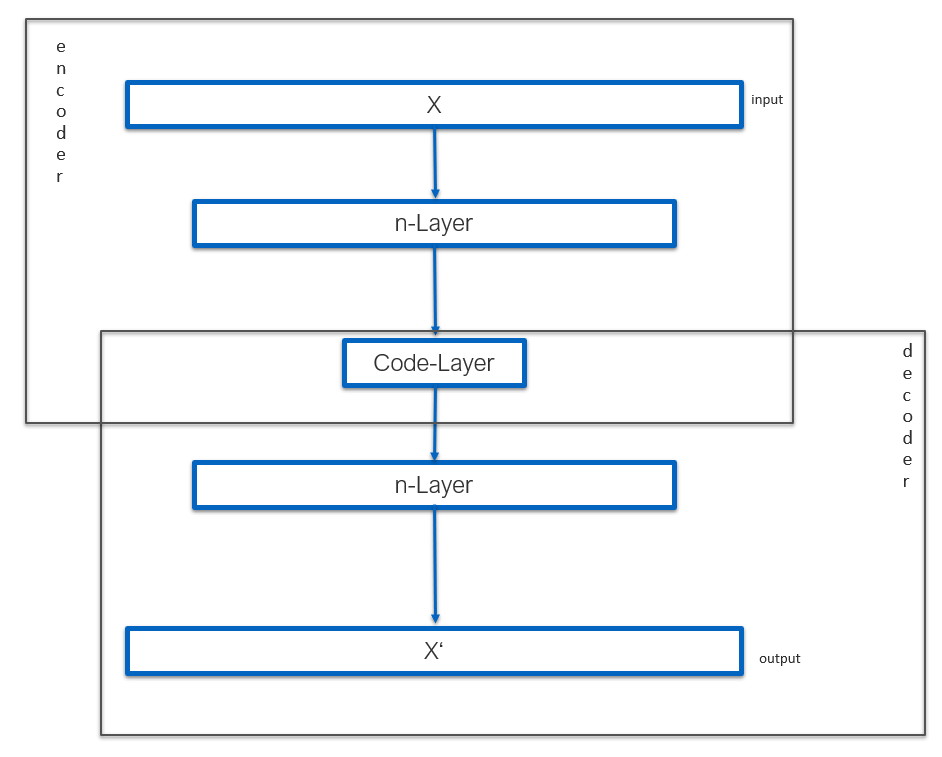
\includegraphics[width=0.7\textwidth, center]{bilder/Schema_Autoencoders/Schema_CAE2.png}
				\caption[Schema Autoencoder]{Schema Autoencoder}
				\label{img:SchemaCAE}
			\end{figure} 
	In der einfachsten Form besteht ein Autoencoder aus einer Eingabeschicht, einer versteckten Schicht und eine Ausgabeschicht. Sie können aber auch mit mehreren Schichten, also mit 'tiefen Architekturen' genutzt werden. \cite{Hinton.2006}
	Der Encoder lässt sich auch vereinfacht als die Funktion $F(x)=c$ und der Decoder als die Funktion $ F(c)=x'$ darstellen, wobei $x\stackrel{!}{=}x'$ sein soll. 
	Autoencoder gibt es in vielen verschiedenen Ausführungen. Dabei sind die meisten Typen von Autoencoder unvollständige Autoencoder. Die verborgene Schicht, das Codelayer enthält weniger Informationen als die Eingabe. Hierdurch wird die Dimensionsreduzierung erzwungen. Andere Aufgaben können Entrauschung mittels Denoising autoencoder \cite{Vincent.2008} oder Generierung neuer Datenpunkte mittels Varrational Autoencoder \cite{Kingma.2019} sein. Contractive Autoencoder \cite{Rifai.2011} nutzen einen Regularisierer in der Zielfunktion, um das Modell zu zwingen eine Funktion zu lernen, die flexibler auf Variationen der Eingabewerte reagiert.   	

	Für die Arbeit ist der \acl{cae} \cite{Masci.2011} kurz \ac{cae} interessant. Er ist ist ein Stacked Autoencoder, welcher Faltungsschichten (Convolutional Layer)  integriert. Faltungsschichten kommen von \cite{LeCun.1999} und haben sich durchgesetzt \cite{Krizhevsky.2012}, \cite{ChristianSzegedy.2014}  und \cite{LeCun.2015}. 
	
	\paragraph{Schichtenweise Vortrainieren} Im schichtenweise Vortrainieren \cite{Bengio.2007}  werden einzelne Schichten eines neuronalen Netzwerkes vor dem eigentlichen Training trainiert, um die Leistung des gesamten Models zu erhöhen. Bei (symmetrischen) Autoencodern werden dabei die zueinander symmetrischen Schichten des Encoders und Decoders miteinander trainiert. Die Zielgröße ist dabei die Rekonstruktion der Eingabedaten.    

	\section{ Transferlernen}
	\label{sec:Transferlernen}
	Im traditionellen maschinellem Lernen wird pro Aufgabe und Datenset ein isoliertes Modell erstellt. Das Transferlernen hat das Ziel Wissen zu teilen. Die Isolation der Modelle soll aufgehoben werden. Dabei erfolgt eine Aufteilung in Quell- und Zieldomäne.
	
		\subsection{Tiefes Transferlernen}
		Geprägt durch die Entwicklung hin zu tiefen neuronalen Netzwerken wurden Methoden zum Tiefen Transferlernen (deep transfer learning) vorgeschlagen. \cite{Tan.2018} ordnet diese in vier Kategorien ein. Für eine Einordnung von klassischen Methoden des Transferlernens eignet sich die Erhebung \cite{FuzhenZhuang.2019}.
		     
		\paragraph{Instanzbasiert} Instanz-basierte Ansätze ergänzen, mittels geeigneter Strategie, Gewichte in der Zieldomäne mit Gewichten aus der Quelldomäne.
		\paragraph{Abbildungbasiert} Abbildungs-basierte Ansätze bilden Instanzen aus der Quell- und Zieldomäne in einen neuen Datenraum ab. In dem neuen Datenraum sind die Instanzen aus den zwei Bereichen ähnlich und können für ein gemeinsames Training eines tiefen neuronales Netzwerk genutzt werden. 
		\paragraph{Netzwerkbasiert} Der netzwerkbasierte Ansatz verwendet einen Teil des in der Quelldomäne trainierten Netzwerkes in der Zieldomäne wieder. Es werden dabei sowohl die Netzstruktur als auch die Verbindungsparameter übernommen. Die Netzwerke werden dabei in zwei Teile unterteilt. Der erste Teil ist die sprachunabhängige Merkmalstransformation, der zweite Teil ist der sprachabhängige Klassifikator. Dabei kann die sprachunabhängige Merkmalstransformation in der Zieldomäne wiederverwendet werden. Insbesondere in \cite{JasonYosinski.2014}, \cite{Long.2016} , und \cite{George.2018} hat sich dieser Ansatz bewährt.
		
		\paragraph{Gegnerischbasiert} Gegenerischbasiertes tiefes Transferlernen ist von dem Ansatz erzeugende gegnerische Netzwerke (Generative Adversarial Networks) \cite{IanJ.Goodfellow.2014} inspiriert. Es werden übertragbare Repräsentationen gesucht, die sowohl auf die Quell- als auch auf die Zieldomäne anwendbar sind.

		\subsection{Halbüberwachtes Lernen}
		Halbüberwachtes Lernen ist eine Methode, die sich zwischen unüberwachtem und überwachtem Lernen einordnen lässt. Methoden des unüberwachten Lernens arbeiten komplett ohne annotierte Daten, während überwachtes Lernen mit vollständig annotierten Daten arbeitet. Das halbüberwachte Lernen arbeitet mit teilweise annotierten Daten. Die Anzahl der nicht annotierten Daten übersteigt, in der Regel, die Menge der annotierten Daten. Diese Technik reduziert Annotationskosten durch den Einsatz weniger Daten mit Annotationen. Zu beachten ist dabei, dass sowohl die Beschrifteten als auch nicht beschriftete Daten aus der gleichen Verteilung entnommen werden. 
		Im Gegensatz dazu sind bei dem Transferlernen die Datenverteilungen der Quell- und Zieldomäne oft unterschiedlich.
		\cite{Chapelle.2010} 
				
		\subsection{Multi-Task-Lernen}
		Werden mehrere Aufgaben parallel gelernt spricht man von dem \acl{mtl} kurz \ac{mtl}.Der Begriff \ac{mtl} wurde insbesondere von \cite{Caruana.1998} geprägt. Ziel ist es, Wissen durch gleichzeitiges Lernen einiger verwandter Aufgaben weiterzugeben. Es wird davon ausgegangen, dass das Lernen einer Aufgabe das Lernen der anderen Aufgaben verbessert. Im Allgemeinen wird dies durch das Lernen aller Aufgaben gemeinsam erreicht, wobei die korrelierten Informationen zwischen den einzelnen Aufgaben genutzt werden. Die Aufgaben erzeugen dabei eine niedrigdimensionale Repräsentation, welche dann durch das parallele Lernen besser generalisiert. In manchen Fällen hat sich zudem herausgestellt, dass Multi-Task-Lernen zum Lernen von nicht verwandten Aufgaben vorteilhaft ist.
		Basierend auf den Ein- und Ausgängen wird \ac{mtl} von \cite{Thung.2018} in drei Fälle unterteilt. 
 		
 		\paragraph{Single-Input Multi-Output} SIMO wird verwendet, um aus einer Eingabe Vorhersagen von verschiedenen Arten von Ausgabezielen zu treffen. Diese Art des \ac{mtl} wird auch Mehrklassen-Lernen (multi-class learning) genannt.
		
		\paragraph{Multi-Input Single-Output} MISO bedeutet es werden mehrere Eingaben zum Vorhersagen eines Ausgabezieles genutzt.
	
		\paragraph{Multi-Input Multi-Output} MIMO bedeutet es werden mehrere Eingaben zum Vorhersagen von verschiedenen Arten von Ausgabezielen genutzt.
		
		\begin{figure}[h]
			\centering
			\begin{subfigure}[c]{0.6\textwidth}			
				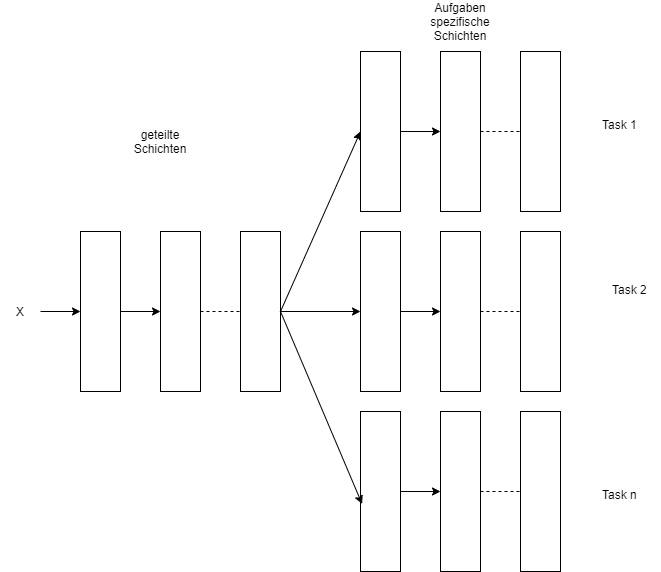
\includegraphics[width=1\textwidth, center]{bilder/Grundlagen/MTL/MTL_SIMO.png}
				\caption[MTL-SIMO]{Single-Input Multi-Output}
				\label{img:MTL_SIMO}	
			\end{subfigure}
			\begin{subfigure}[c]{0.49\textwidth}			
				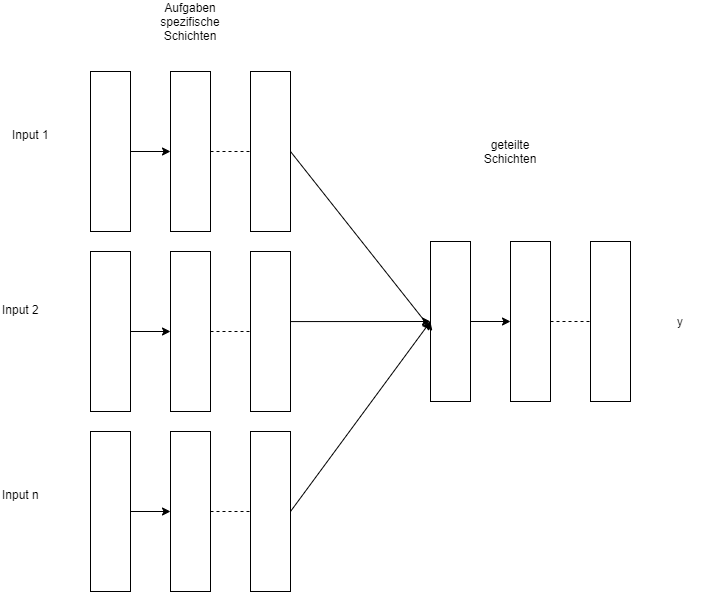
\includegraphics[width=1\textwidth, center]{bilder/Grundlagen/MTL/MTL_MISO.png}
				\caption[MTL-MISO]{Multi-Input Single-Output}
				\label{img:MTL_MISO}	
			\end{subfigure}
			\begin{subfigure}[c]{0.49\textwidth}			
				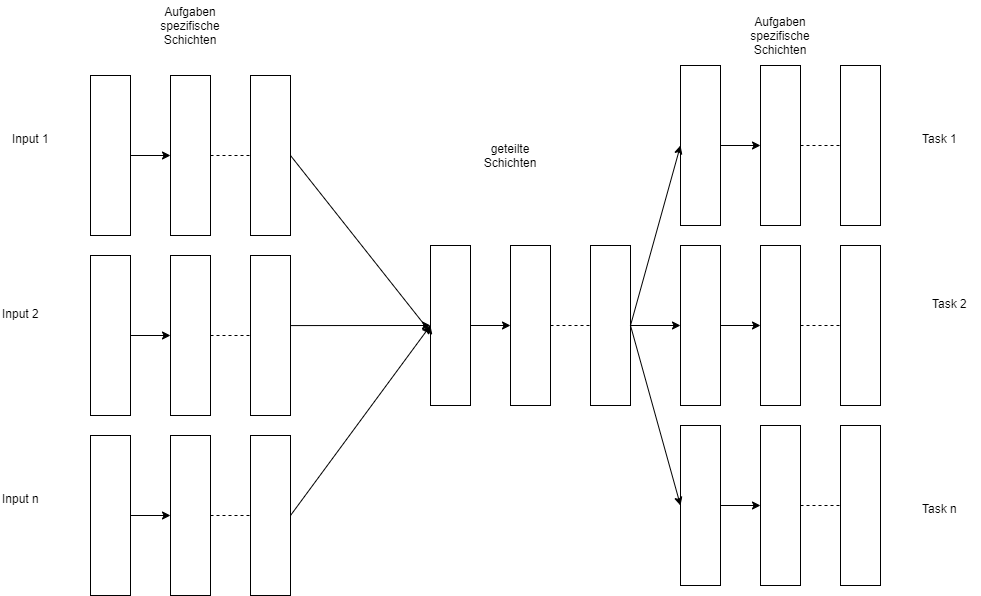
\includegraphics[width=1\textwidth, center]{bilder/Grundlagen/MTL/MTL_MIMO.png}
				\caption[MTL-MIMO]{Multi-Input Multi-Output}
				\label{img:MTL-MIMO}	
			\end{subfigure}
			\caption{Multi-Task-Lernen: Ausprägungen}
			\label{img:MultiTaskLernen}
		\end{figure}
		Abbildung \ref{img:MultiTaskLernen} zeigt die verschiedenen Ausprägungen künstlicher neuronaler Netze, die auf \ac{mtl} beruhen.
		
		Induktives Transferlernen und \ac{mtl} wird darin unterschieden, dass beim induktiven Transferlernen angenommen wird, dass es eine Hauptaufgabe und eine Nebenaufgabe gibt. Die Nebenaufgabe bietet zusätzliche Informationen, um die Hauptaufgabe zu verbessern, bzw. zu generalisieren. Im \ac{mtl} gibt es keine solche Unterscheidung, die Aufgaben werden gleichberechtigt betrachtet. Induktives Transfer-Lernen kann deshalb als Sonderform des \ac{mtl} gesehen werden. 
		
		Die Kombination von Multi-Task-Learning tiefen Lernen für die Computervision wurde in \cite{YuchunFang.2017}, \cite{Li.2016}, \cite{RajeevRanjan.2016} und \cite{Zhao.2019} eingesetzt.

	\section{Automatisiertes maschinelles Lernen}
	\label{sec:AutoML}
	Das \acl{automl} kurz \ac{automl} hat das Ziel alle Aspekte des maschinellen Lernens und der Datenanalyse-Pipeline zu automatisieren. Die vollständige Automatisierung erlaubt es auch Nutzern, ohne oder mit geringen Kenntnissen von ML-Techniken, die Erstellung von ML-Systemen durchzuführen.
	Die vollständige Automatisierung ist ein langfristiges Ziel. Aktuelle Systeme sind halbautomatisch und zielen darauf ab, Personenaufwände bei Bedarf nach und nach durch Rechenvorgänge zu reduzieren. Trotz der steigenden Rechenleistung, können AutoML-Methoden sehr rechenintensiv sein.  \ac{automl} wird in drei Methoden eingeordnet. Das Meta-Learning, \acl{nas} kurz \ac{nas} und \acl{hpo} kurz \ac{hpo}. 
	\cite{Hutter.2019} 
	
	\subsection{\acl{hpo}}
	\label{subsec:HyperparameterOptimierung}	
	Hyperparameter sind alle Parameter, welche vor Beginn des Trainings zur Steuerung des Trainings eingestellt werden können. Eine passende Einstellung dieser Parameter beeinflusst die Leistung eines Modells maßgeblich. In \cite{Kohavi.1995} wurde festgestellt, dass verschiedene Hyperparameterkonfigurationen für verschiedene Datensätze am besten funktionieren. Es ist also notwendig für jede Aufgabe aufs Neue die beste Hyperparameterkonfiguration zu finden.      
	Automatische-\ac{hpo} ist die Technik des automatischen Finden der Hyperparameter, um die Leistung zu optimieren. Dabei hat sie insbesondere drei Ziele: An erster Stelle sollen Personenaufwände bei der Anwendung von maschinellem Lernen reduziert werden, zusätzlich soll es die Leistung von Algorithmen und Modellen des maschinellen Lernens verbessern. Des Weiteren sollen so in der Wissenschaft die Reproduzierbarkeit und Fairness von Studien verbessert werden, da Automatische-\ac{hpo} einfacher reduzierbar ist, als manuelle-\ac{hpo}. In Kapitel \ref{subsec:Optimierungstechniken} werden einige gängige Optimierungstechniken der automatischen-\ac{hpo} erläutert.  
	\cite{Feurer.2019}		
	
	
	\subsection{Meta-Learning}
	\label{subsec:MetaLearning}
	Unter \cite{JoaquinVanschoren.2018} ist eine Übersicht über das Meta-Learning zu finden. In dieser Arbeit wird das Thema nur vollständigkeitshalber aufgelistet. Meta-Learning umfasst jede Art von Lernen, welches auf frühere Erfahrungen zurückgreift. Dabei können umso mehr Arten von Metadaten genutzt werden je ähnlicher die Aufgaben sind. Metadaten sind dabei alle Daten, die frühere Lernaufgaben beschreiben. Dies können z.B Algorithmuskonfigurationen, Hyperparameter, Netzarchitekturen, Modellbewertungen und vieles mehr sein.
	
	\subsection{Neural Architecture Search}
	\label{subsec:NeuralArchitectureSearch}
	Im Deep Learning hängt die Leistung eines Modells maßgeblich von der genutzten Architektur ab. Das manuelle Suchen von Architekturen ist zeitaufwendig und fehleranfällig. Die Neural Architecture Search befasst sich damit, wie Architekturen automatisch gefunden werden können. In dieser Arbeit wurde nicht auf die Technik der Neural Architecture Search zurückgegriffen und das Thema ist nur vollständigkeitshalber aufgeführt. Unter \cite{Elsken.2019} kann eine Übersicht über die Neural Architecture Search gefunden werden. 	

	\subsection{Optimierungstechniken}
	\label{subsec:Optimierungstechniken}
	In diesem Unterkapitel werden gängige Optimierungsmethoden des \ac{automl} dargestellt. Die Auflistung ist nicht vollständig, deckt aber die im praktischen Teil der Arbeit zur Verfügung stehenden Methoden ab.  
	
	\paragraph{Rastersuche}
	Die Rastersuche \cite{Michelucci.2018} ist eine modellunabhängige Optimierunsstrategie. Es werden Parameterkombinationen definiert und anschließend Modelle, ausgehend von den Kombinationen, erstellt und evaluiert. Diese Technik hat einige Schwächen, so müssen Parameterkombinationen definiert werden, jedes Modell muss trainiert werden und falls die optimale Konfiguration nicht enthalten ist, wird sie nie gefunden. 
	
	\paragraph{Zufallssuche}
	Die Zufallssuche ähnelt der Rastersuche. Sie unterscheidet sich dahingehend, dass die Parameterkombinationen nicht mehr definiert werden müssen. Es werden zufällige Stichprobenkonfigurationen aus dem (definierten) Parameterraum gezogen und evaluiert. 
	In \cite{BergstraJamesandYoshuaBengio..2012} wurde gezeigt, dass insbesondere bei unterschiedlicher Wichtigkeit der Hyperparameter, bessere Ergebnisse erzielt werden. 

	\paragraph{Bayesian optimization}
	Bayesian optimization ist ein Ansatz der zur Optimierung von Zielfunktionen dient, die eine lange Zeit (Minuten oder Stunden) zur Auswertung benötigen. Im Gegensatz zur Rastersuche oder Zufallssuche ist der Ansatz modellabhängig. Der Ansatz ist iterativ und baut auf zwei Komponenten auf. Ein probabilistisches Ersatzmodell und eine Erfassungsfunktion, die zur Bewertung, welcher Punkt als nächstes bewertet werden soll, herangezogen wird. Das Ersatzmodell wird in jeder Iteration an alle Beobachtungen angepasst. Im Gegensatz zur Blackboxfunktion, ist die Auswertung der Erfassungsfunktion billig und kann somit zur Optimierung herangezogen werden.
	\cite{Frazier.201807}
			
	\paragraph{Hyperband}	
	Hyperband \cite{Li.2017} erweitert \acl{sh} \cite{Jamieson.2015}. \acl{sh} kurz \ac{sh} weist einer Reihe von Hyperparameter-Konfigurationen eine einheitliche Menge an Ressourcen zu, berechnet die Leistung von allen Konfigurationen und entfernt die schlechtere Hälfte. Die Konfigurationen werden dabei zufällig gezogen. Das Ganze wird wiederholt, bis eine Konfiguration übrig bleibt. In jedem Durchlauf wird der übriggebliebenen Hälfte exponentiell mehr Ressourcen zugewiesen. \ac{sh} benötigt als Eingangsparameter die Ressourcen und die Anzahl an Konfigurationen. Dabei ist es schwierig, zu entscheiden, ob wenige Konfigurationen mit mehr Ressourcen oder viele Konfigurationen mit weniger Ressourcen durchgeführt werden sollen.
	Hyberband erweitert \ac{sh}, um dieses Problem zu adressieren. Hyperband führt eine Rastersuche für die beiden Parameter durch. Es werden also mehrere \ac{sh}-Durchläufe mit diversen Konfigurationen durchgeführt. Die Anzahl an Konfigurationen wird dabei immer weiter reduziert. Abgeschlossen wird eine Ausführung mit einer Zufallssuche.
	
	\paragraph{BOHB}
	BOHB \cite{StefanFalkner.2018} ist ein Ansatz, der Bayesian optimization und Hyperband kombiniert. Dabei wird Bayesian optimization zur Auswahl von Konfigurationen herangezogen und Hyperband bestimmt wieviele Konfigurationen, mit welchem Budget ausgeführt werden sollen. Anschließend werden die Konfigurationen mittels Successive Halving ausgeführt. Unter https://github.com/automl/HpBandSter kann eine Implementierung des Werkzeuges gefunden werden. Diese Framework wurde für den praktischen Teil der Arbeit genutzt.
			
	\section{Bibliotheken und Werkzeuge}
	\label{sec:BibliothekenundWerkzeuge}
	Für den praktischen Teil der Abschlussarbeit wurde insbesondere Cnvrg \cite{cnvrg.io.2020} genutzt. Cnvrg.io ist eine 'full-stack' Data Science Platform, welche Werkzeuge für die Erstellung, Verwaltung, Bereitstellung und Automatisierung von maschinellem Lernen bereitstellt. Cnvrg erlaubt es Arbeitsbereiche mittels Container zu erstellen. Die Container können dabei auf Maschinen in Azure \cite{Micorsoft.2020} zugreifen. Für die Experimente wurde ein vorgefertigter Container mit einer tesla-k80 \cite{Nvidia.2020}, fünf CPUs und 49 GB Arbeitsspeicher genutzt. 

	Für die Entwicklung wurden Python \cite{PythonSoftwareFoundation.2020}, Jupyter Notebooks \cite{ProjectJupyter.} und das Framework Tensorflow \cite{MartinAbadi.2015}  genutzt. Die wichtigsten Bibliotheken für die Arbeit sind Keras \cite{Chollet.2015} , Numpy \cite{Oliphant.2006} , Matplotlib \cite{Hunter.2007} , scikit-learn \cite{Pedregosa.2011} , ConfigSpace \cite{Lindauer.2019} , Bayesian Optimization and Hyperband \cite{StefanFalkner.2018}. 
	
	Für die Visualisierung von Bildeinbettungen wurde die Software 'PSIORI Visualizer' erweitert und eingesetzt. Die Software erlaubt es dreidimensionale Daten darzustellen. Dabei können Filter eingesetzt sowie Blickwinkel geändert werden, Daten können mit zusätzlichen Informationen versehen werden und Zoomen ist möglich. Als zusätzliche Information können z.B. ein Originalbild und seine Rekonstruktion oder die Information, ob eine Vorhersage korrekt oder falsch war hinterlegt werden.
	
	Kern der erstellten Softwaremodule ist das Framework  Psipy \cite{PSIORIGmbH.2019}. Psipy ist ein Python-Framework für maschinelles Lernen, welches von PSIORI selbst entwickelte Werkzeuge zusammenfasst und unter einer einheitlichen API zu Verfügung stellt. Diese API ist an die API des verbreiteten Frameworks scikit-learn angelehnt. Es können Modelle basierend auf scikit-learn  und Tensorflow eingebunden werden. In den nachfolgenden Abschnitten werden die, für die Arbeit, wichtigsten bestehenden Module des Frameworks vorgestellt.
	
	 \paragraph{saveable.py} Das Modul saveable ist eine flexible Basisklasse, die Kernfunktionalität zum Speichern und Laden von Python-Objekten bietet. Es können Modelle, welche diverse Bibliotheken nutzen, auf eine einheitliche Art und Weise gespeichert werden. Um die Klasse Saveable nutzen zu können, müssen erbende Klassen ihre Konstruktorargumente an die Basisklasse übergeben. Zusätzlich ist es notwendig eine Erweiterung beim Speichern und Laden zu implementieren. Beim Speichern ist es notwendig eine Erweiterung, um alle (meist ein) Module und weitere Argumente zu implementieren. Beim Laden müssen die gespeicherten Module und Argumente geladen werden. In Listing \ref{lst:SaveTensorflow} ist die Erweiterung zum Speichern eines Tensorflow-Models abgebildet. 
	\begin{lstlisting}[language=python,caption=Erweiterung zum Speichern eines Tensorflow Models, label=lst:SaveTensorflow]
		...
		zip_file.add("model.h5", self.model)
		...
	\end{lstlisting}

	\paragraph{autoencoder.py} Das Modul autoencoder enthält die drei Klassen StackedAutoencoder, FullyConnectedAutoencoder und ConvolutionalAutoencoder. Der StackedAutoencoder wird als Basisklasse für die anderen beiden Klassen genutzt. Im Konstruktor werden Methoden aufgerufen, welche in den abgeleiteten Klassen ausprogrammiert sind. Dabei wird ein Keras-Modell für einen Encoder und Decoder entsprechend von Parametern erstellt. Als weitere wichtige Methoden gibt es die Methode $pretrain(..)$ und $fit(..)$. Mittels $pretrain(..)$ werden die Schichten eines symmetrischen Autoencoder von außen nach innen wie, in \cite{Bengio.2007} beschrieben vortrainiert. Die Zuordnung der Schichten erfolgt in den abgeleiteten Klassen.
	In der $fit(..)$-Methode wird nach einigen Prüfungen die Methode f$fit(..)$ \cite{Chollet.2015} des Kerasmodels aufgerufen. In Abbildung \ref{img:KlassendiagrammConvolutionalAutoencoder} ist das Klassendiagramm mit den öffentlichen Methoden des ConvolutionalAutoencoder dargestellt. 
	\begin{figure}[h]
		\centering
		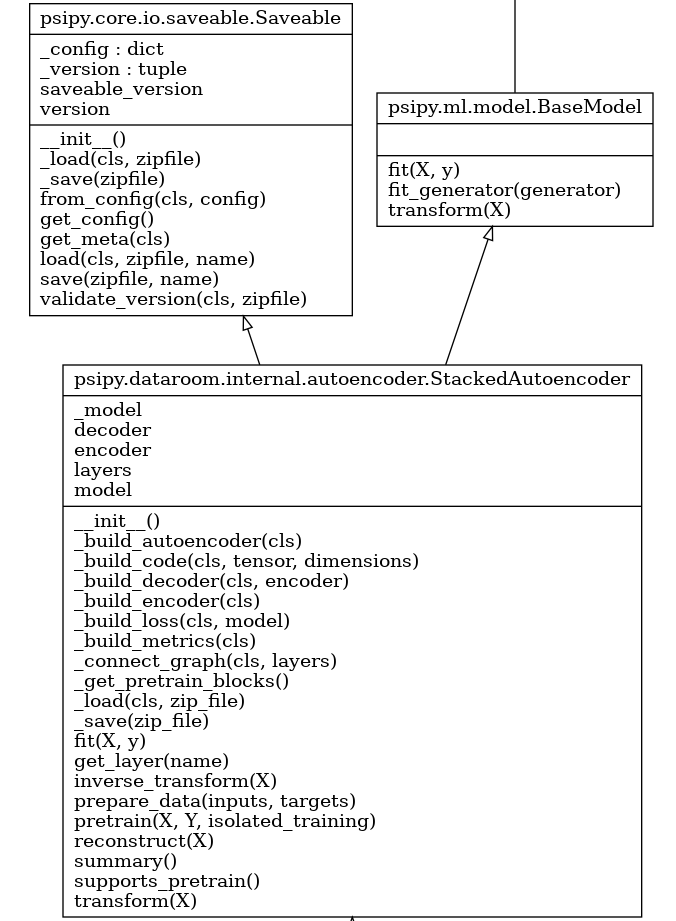
\includegraphics[width=0.6\textwidth, center]{bilder/Klassendiagramme/klassendiagramm_public_cae2.png}
		\caption[Klassendiagramm ConvolutionalAutoencoder]{Klassendiagramm ConvolutionalAutoencoder}
		\label{img:KlassendiagrammConvolutionalAutoencoder}
	\end{figure}  
	
	\paragraph{hyperparameter\_mixin.py}  Hyperparameter\_mixin wird zum standardisierten Verwalten von Hyperparametern für AutoML-Klassen genutzt. Auf die Hyperparameter kann anschließend einheitlich zugegriffen werden. Abbildung \ref{img:KlassendiagrammHyperparametermixin} zeigt das zugehörige UML-Klassendiagramm mit den Methoden zum Hinzufügen, Löschen und Laden der Hyperparameter. Da die Methoden öffentlich sind, können über jede erbende Klasse die Hyperparameter eigenständig verwaltet werden.	
	\begin{figure}[h]
		\centering
		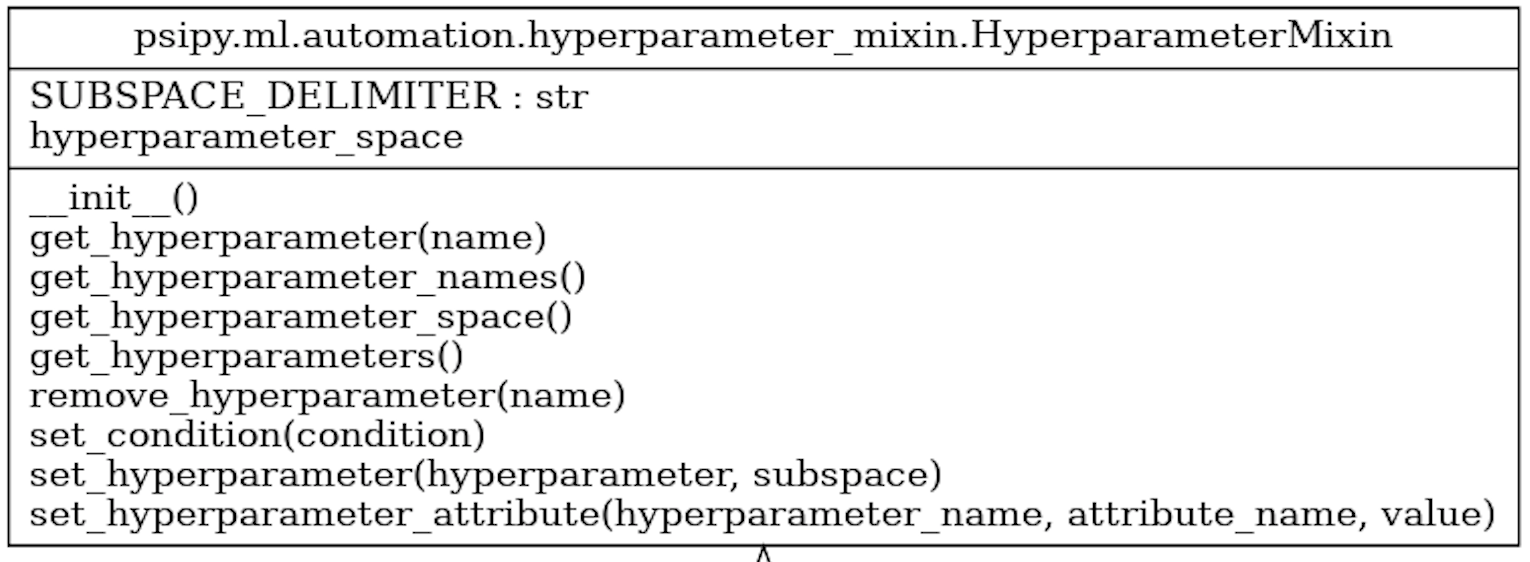
\includegraphics[width=0.6\textwidth, center]{bilder/Klassendiagramme/Hyperparametermixin.png}
		\caption[Klassendiagramm Hyperparametermixin]{Klassendiagramm Hyperparametermixin}
		\label{img:KlassendiagrammHyperparametermixin}
	\end{figure}  
	
	\section{Einordnung und bestehende Systeme}
	\label{sec:BestehendesSystem}
	Die Bilddaten und Aufgabenstellungen der neuronalen Netzwerke sind in die Problemstellungen des Autocrane-Projekts \cite{PSIORIGmbH.2020} von PSIORI einzuordnen. Es sind echte Datensätze und echte Problemstellungen, wobei die gezeigten Aufgabenstellungen und Modelle nicht zwingend in dem Autocrane-Projekt zum Einsatz kommen. Das Autocrane-Projekt ist ein (laufendes) Projekt, welches das Ziel hat, einen feststehenden Rundlaufkran vollautomatischen zu steuern. In Abbildung \ref{img:CircularCrane} ist ein Rundlaufkran abgebildet. Diese Art von Kran werden in holzverarbeitenden Anlagen zum Befüllen von Fülltrichtern oder Förderbändern eingesetzt. Der Kran kann sich um 360 Grad drehen. Der Greifer kann nach oben, unten und mittels eines Schlittens entlang eines Auslegers bewegt werden. Um die Bilder aufnehmen zu können, wurde an der Kabine am Hauptstandfuß eine Kamera angebracht. Die Kamera ist auf das Ende des Auslegers und den Bereich darunter ausgerichtet. Die Kamera bewegt sich mit dem Rundlaufkra, wodurch der Greifer immer im Bild ist. Für das Autocarne-Projekt sind insbesondere drei Anwendungsfälle interessant. Die Baumstämme werden mittels LKW angeliefert und müssen nach vorgegebenen Regeln (z. B. Ausrichtung, freier Lagerplatz) als Holzstapel gelagert werden. Der Fülltrichter muss mit Holz aus den Holzstapeln befüllt werden. Der Fülltrichter muss mit Holz aus einem LKW befüllt werden. Es ergeben sich Aufgabenstellungen wie Greifer-Erkennung, Baumstamm-Erkennung, LKW-Erkennung, Strategien für das Entladen und Aufbewahren der Baumstämme und vieles mehr. Im Normalbetrieb werden täglich 140-200 LKW entladen. Die Ladung ist 9 - 18 Meter lang und 34 - 40 Tonnen schwer. 
	\begin{figure}[h]
		\centering
		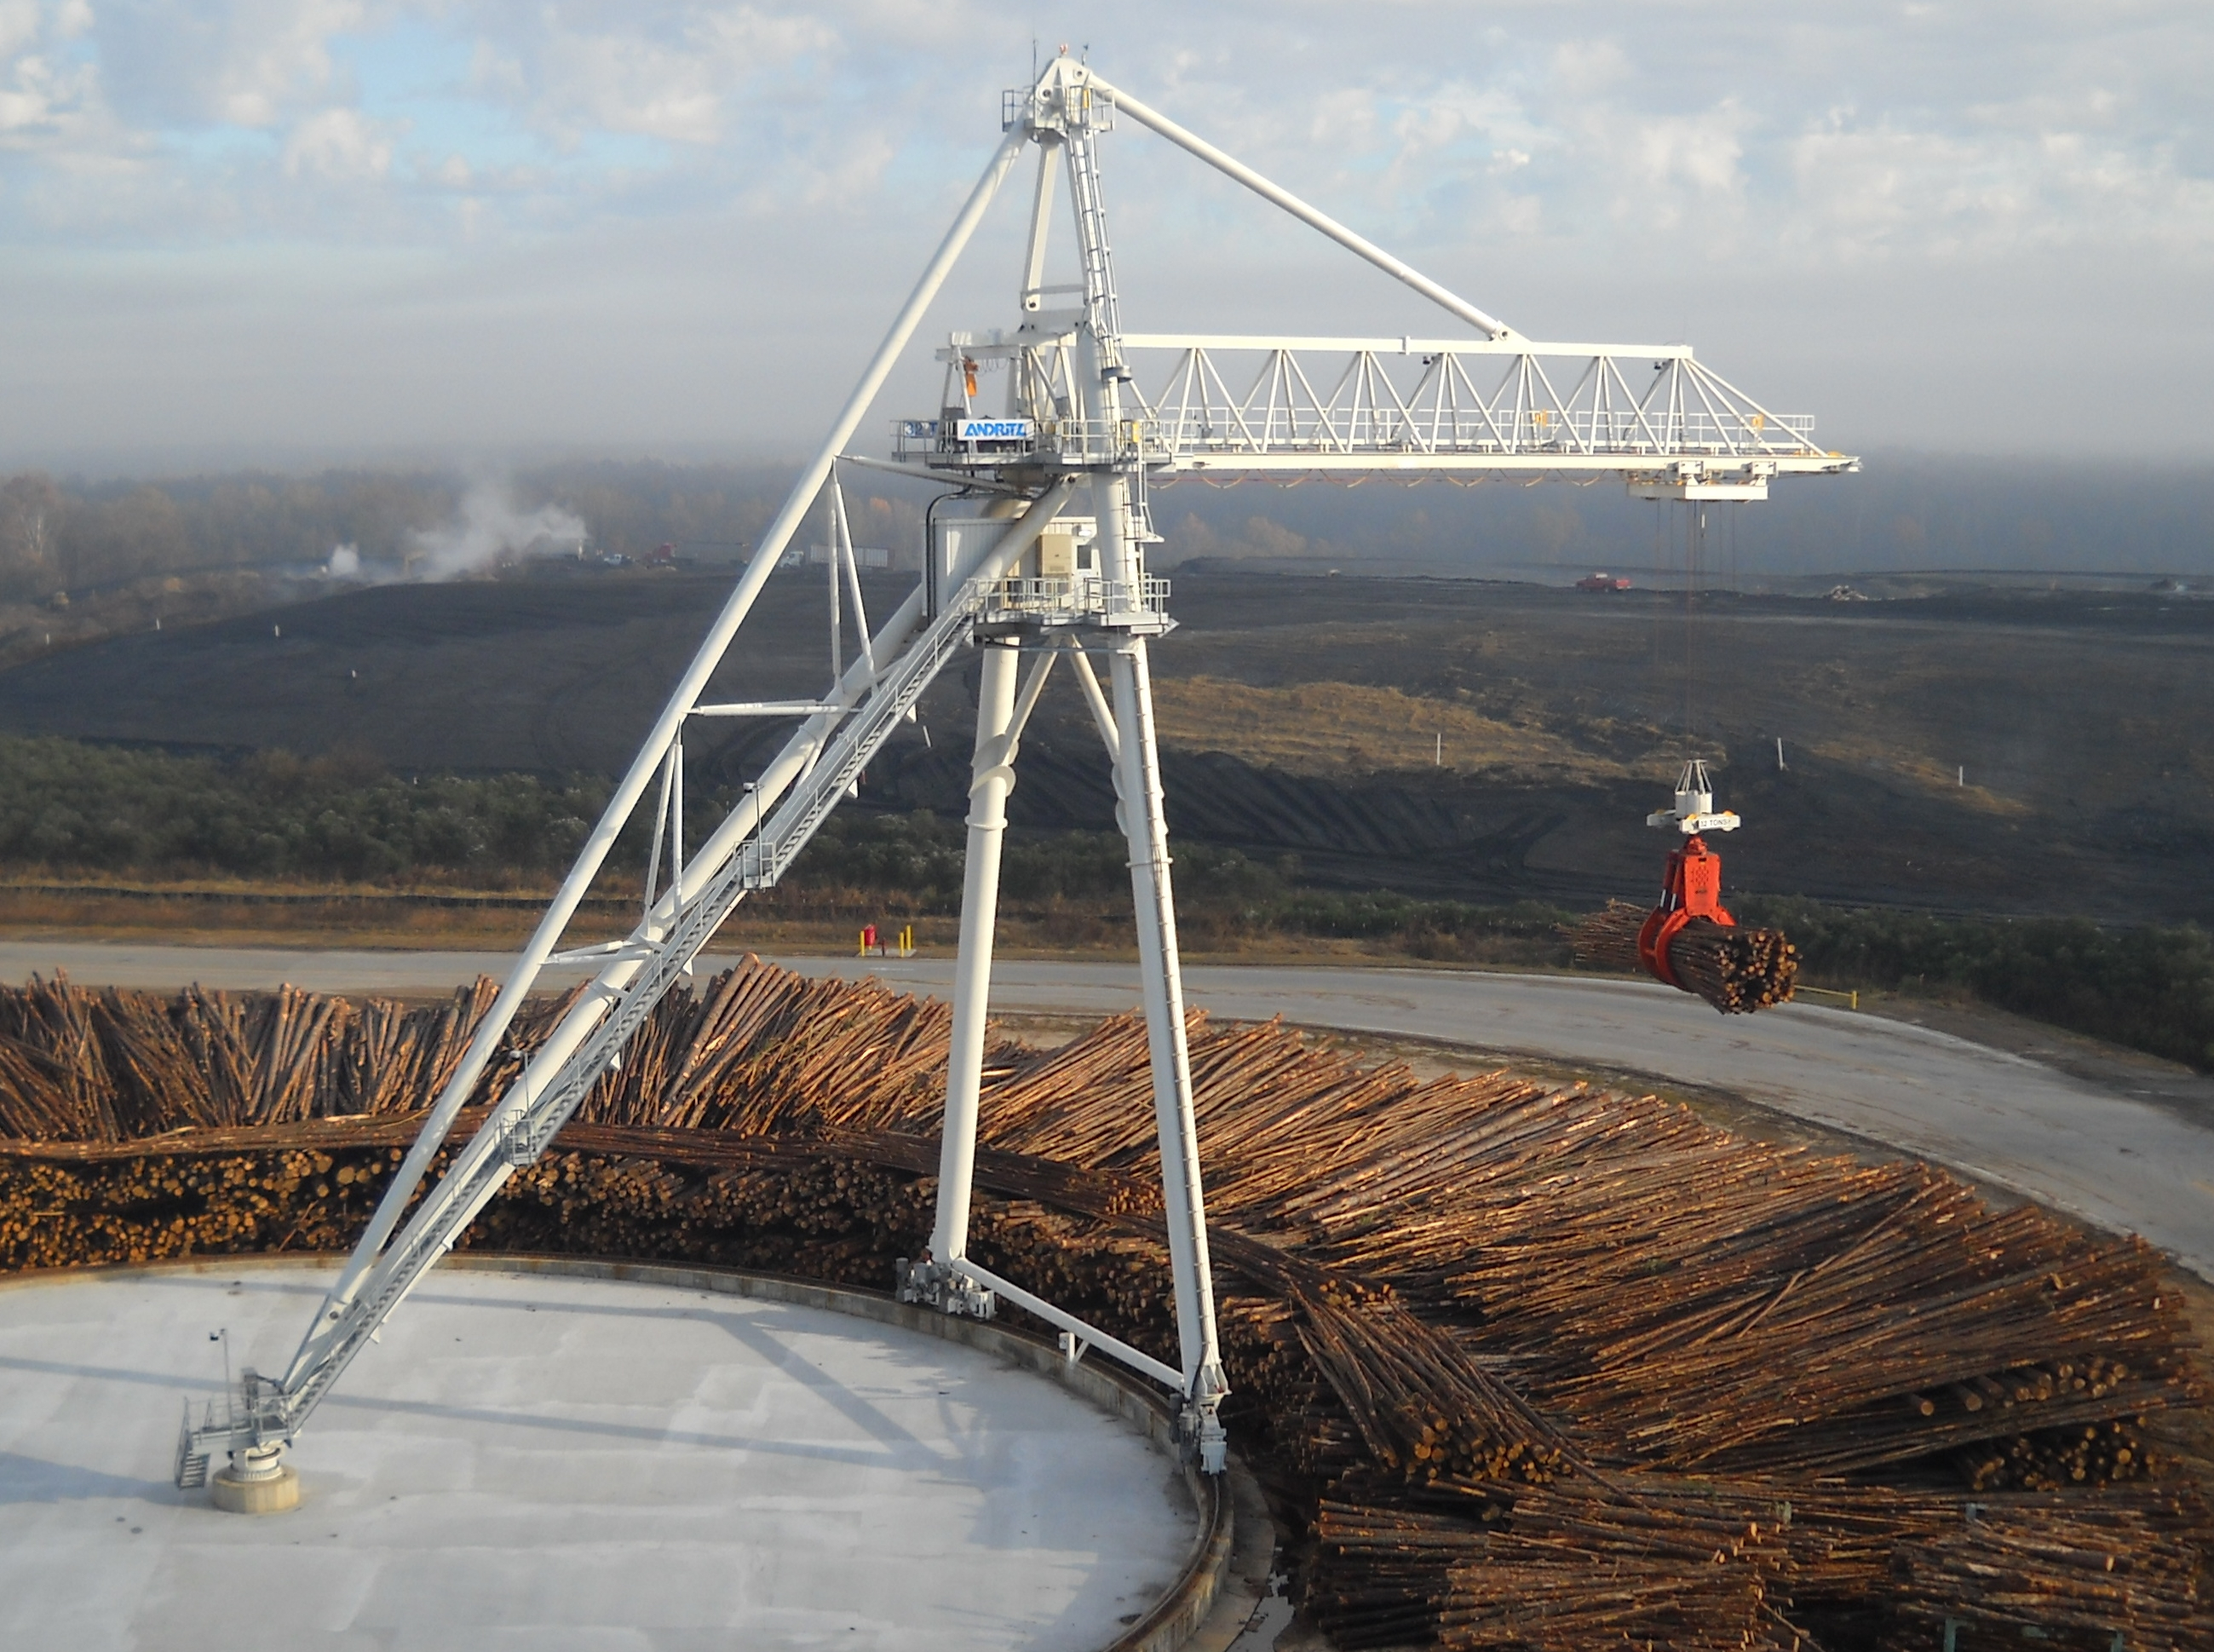
\includegraphics[width=0.5\textwidth, center]{bilder/Grundlagen/Kran_vollstaendig_N1_030.jpg}
		\caption[Rundlaufkran]{Rundlaufkran (Foto: ANDRITZ)}
		\label{img:CircularCrane}
	\end{figure}		

	\paragraph{Greifererkennung} Bei der Aufgabenstellung Greifererkennung muss in einem Bild die Position eines Rahmen um den Greifer gefunden werden. Abbildung \ref{img:Grapple} zeigt ein Bild eines Rahmens um den Greifer. Es handelt sich um eine klassische Objekterkennungs-Aufgabe.
	\begin{figure}[h]
		\centering
		\begin{subfigure}[c]{0.49\textwidth}			
			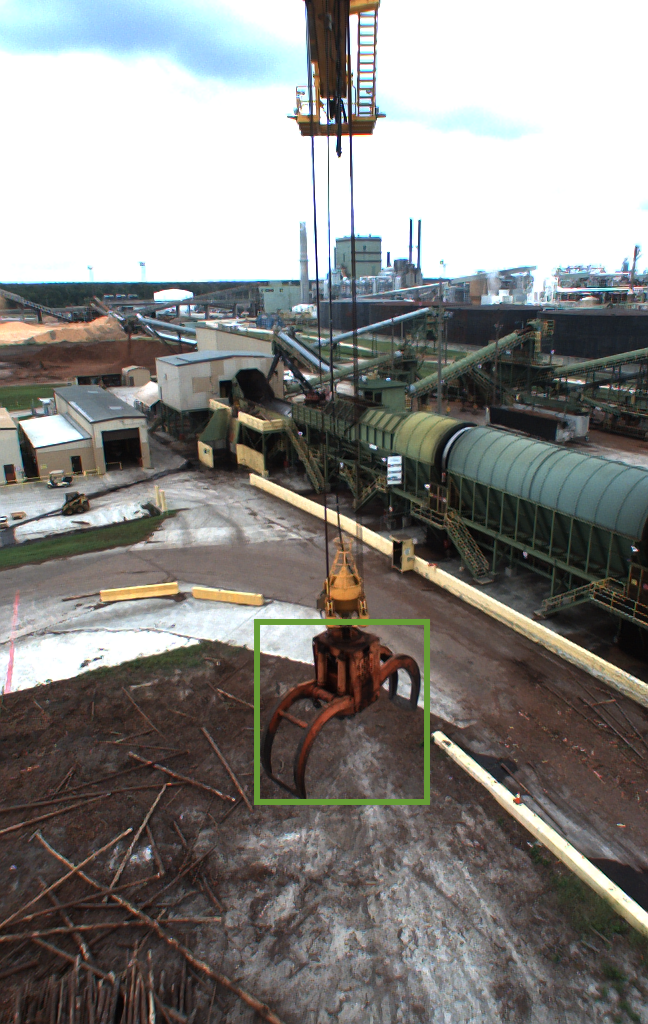
\includegraphics[width=1\textwidth, center]{bilder/Grundlagen/Grapple_8.png}
			\caption[Bsp. Bild: Greifer mit Rahmen]{Greifer mit Rahmen}
			\label{img:Grapple}	
		\end{subfigure}
		\begin{subfigure}[c]{0.49\textwidth}			
			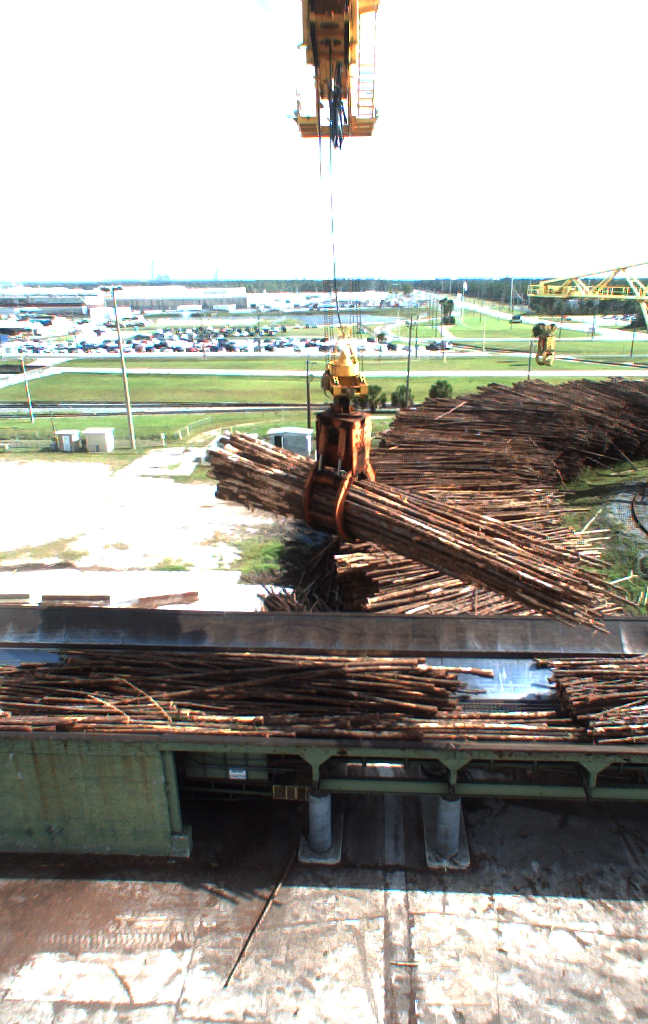
\includegraphics[width=1\textwidth, center]{bilder/Grundlagen/Logs_14.png}
			\caption[Bsp. Bild: Greifer mit Baumstämmen]{Greifer mit Baumstämmen}
			\label{img:Logs}	
		\end{subfigure}
		\caption{Greifer}
		\label{img:Greifer}
	\end{figure}	

	PSIORI hat die Aufgabe mittels neuronalem Netzwerk gelöst. Dabei wurde auf die Technik des \acl{ssd} (\ac{ssd}) \cite{Liu.2015} zurückgegriffen. Die Vorhersagegenauigkeit dieses Modells wird als Basislinie und Vergleichswert genutzt. Dabei ist die ausschlaggebende Metrik die  \acl{iou} kurz \ac{iou} mit einem Schwellenwert von 0.8. Es wird also die Fläche der Überschneidung der beiden Rahmen durch die Gesamtfläche der Rahmen geteilt und wenn ein Wert >= 80\% erreicht wird, als korrekt vorhergesagt eingestuft.  Das Modell erreicht einen Wert von $0.86$. In Anhang \ref{appendix:BasislinieGreifer} ist die vollständige Basislinie dargestellt.
	
	\paragraph{Greifer beladen?} Die Aufgabe 'Greifer beladen?' hat zum Ziel, zu erkennen ob sich Baumstämme im Greifer befinden oder nicht. Es handelt sich um eine Klassifikationsaufgabe. Für diese Aufgabe wurde von PSIORI ein Modell erstellt. Dieses Modell wird wie das Greifererkennungsmodell als Basislinie und Vergleichswert für die durchgeführten Versuche genutzt. Das Modell erreicht auf den Validation-Daten eine Accuracy von 0.9828\%. Im Anhang \ref{appendix:BasislinieBaumstämme} ist die vollständige Basislinie dargestellt. 

	\section{Datenverständnis}
	\label{sec:DataUnderstanding}
	Mittels Kamera an der Kabine können neue unbeschriftete Bilder aufgenommen und bei PSIORI abgelegt werden. Durch den Aufbau des Rundkrans und der Kameraposition, befindet sich der Greifer immer im Bild. Der Hintergrund der Bilder ändert sich stark. Die geografische Lage des Rundkrans schränkt die möglichen Wetterlagen ein. Es fällt kein Schnee und es gibt wenige Regentage. In Abbildung  \ref{img:Bildqualität} sind Ausprägungen der Bildqualität dargestellt. Abgesehen von Bildern in guter Qualität gibt es helle Bilder, dunkle Bilder und Bilder mit Reflexionen. Die Bilder sind 1024 auf 648 Pixel groß und in Farbe. Die einzelnen Pixel können dabei Werte zwischen 0 und 255 annehmen. 
	Entsprechend der beiden Aufgabenstellungen Greifererkennung und 'Greifer beladen' werden Daten mit einer passenden Beschriftung bereitgestellt.
	
	\begin{figure}[h]
		\centering
		\begin{subfigure}[c]{0.24\textwidth}			
			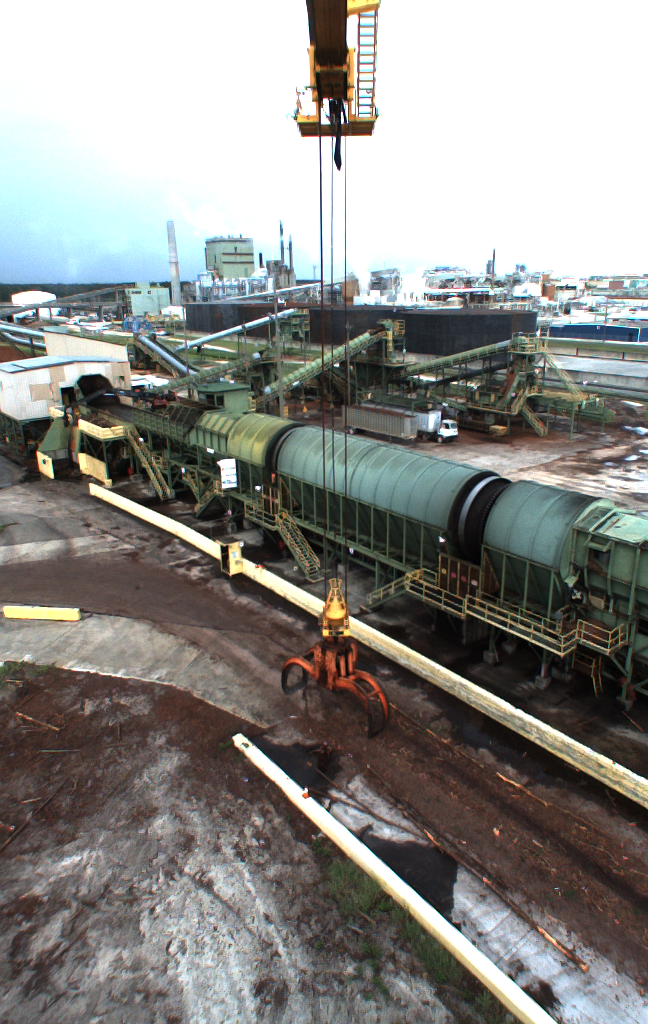
\includegraphics[width=1\textwidth]{bilder/Grundlagen/Daten_Bildqualitaet/gut.png}
			\subcaption{Gut}			
		\end{subfigure}
		\begin{subfigure}[c]{0.24\textwidth}			
			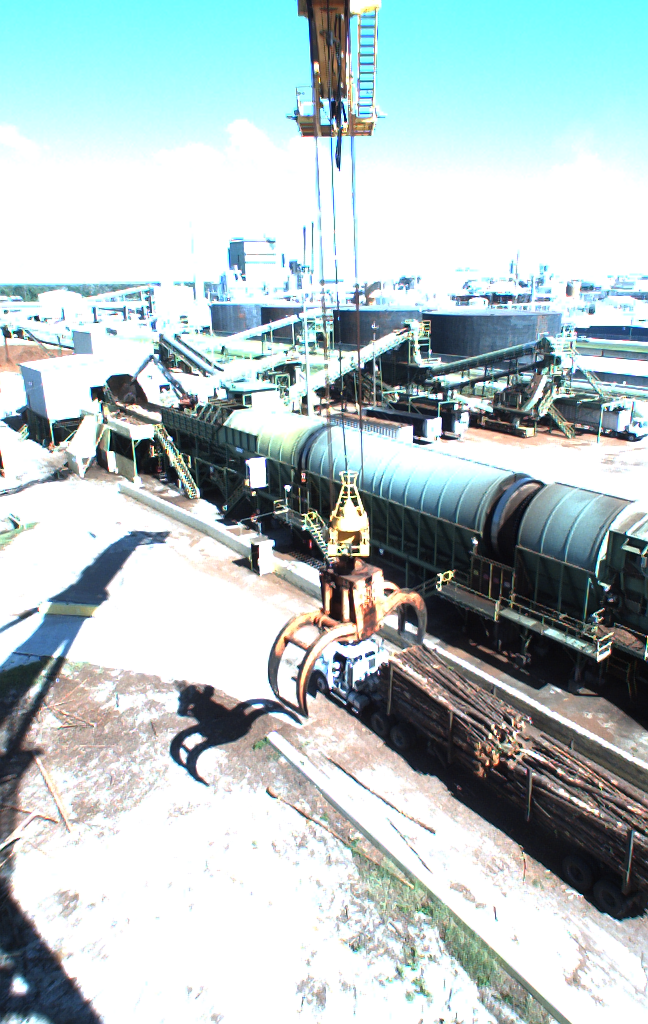
\includegraphics[width=1\textwidth]{bilder/Grundlagen/Daten_Bildqualitaet/hell.png}
			\subcaption{Hell}			
		\end{subfigure}
		\begin{subfigure}[c]{0.24\textwidth}			
			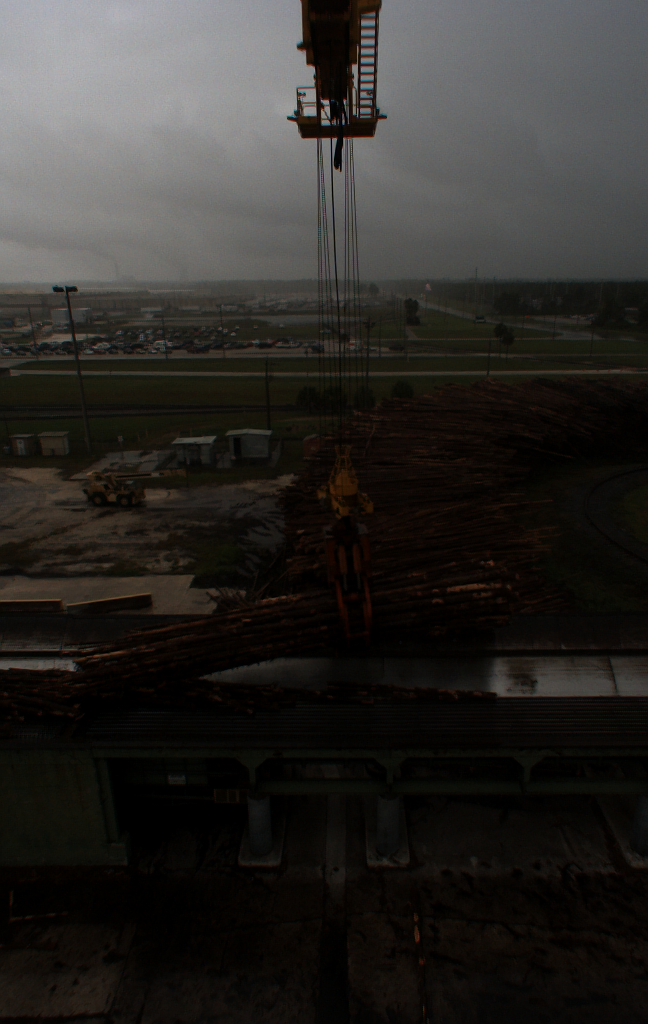
\includegraphics[width=1\textwidth]{bilder/Grundlagen/Daten_Bildqualitaet/dunkel.png}
			\subcaption{Dunkel}			
		\end{subfigure}
		\begin{subfigure}[c]{0.24\textwidth}			
			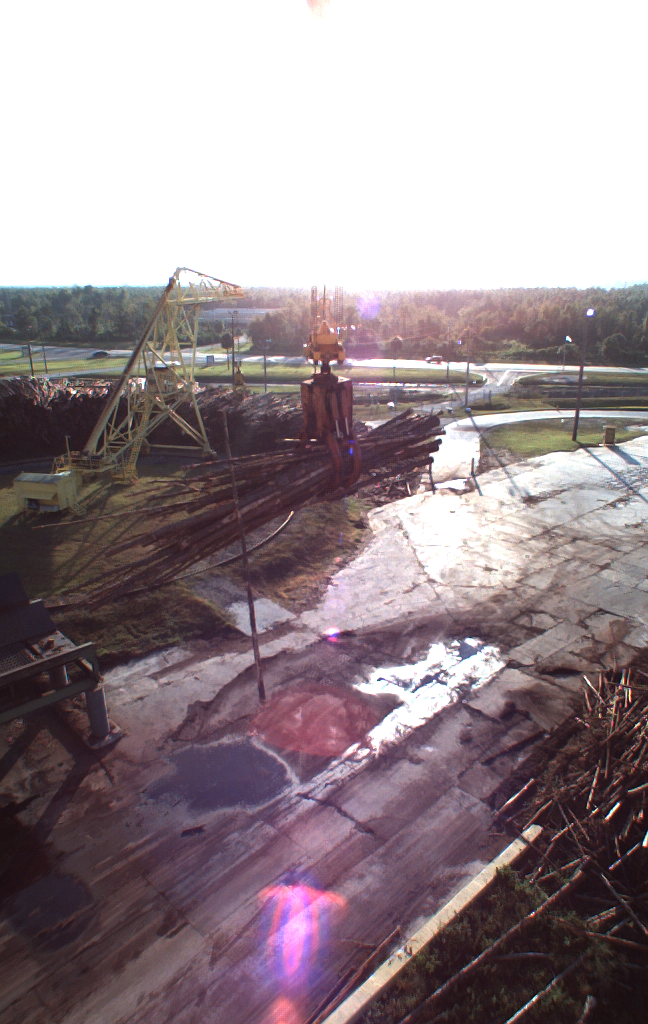
\includegraphics[width=1\textwidth]{bilder/Grundlagen/Daten_Bildqualitaet/Reflexionen.png}
			\subcaption{Reflexionen}			
		\end{subfigure}
		\caption{Bildqualität}
		\label{img:Bildqualität}
	\end{figure}
		
	\paragraph{Greiferdatensatz} Der Greifer Datensatz enthält Bilder, in welchen der Greifer mittels Rahmen markiert ist. Abbildung \ref{img:Grapple} zeigt ein beispielhaftes Bild mit markiertem Greifer. Die Annotationen der Position des Greifers wurde pro Bild in einer XML-Datei abgelegt. Konkret wurde die Position als x, y Koordinaten in der Form ymin, xmin, ymax und xmax abgespeichert. Über die vier Werte lässt sich problemlos ein Rahmen um den Greifer spannen. Der Datensatz besteht aus 4.684 durch Personen annotierten Bildern.
	
	\paragraph{Generierter Greiferdatensatz}  Erfahrungsgemäß lernen Autoencoder Lichtverhältnisse in Bildern relativ gut. Um für erste Versuche den Fokus von den Lichtverhältnissen auf die eigentliche Aufgabenstellung zu setzen wurde ein weiterer Greiferdatensatz erzeugt. Hierfür wurden 8966 Bilder mittels dem Basislinienmodell beschriftet und in 7171 Trainingsdaten und jeweils 896 Test- und Validationsaten aufgeteilt.
	 
	\paragraph{Baumstammdatensatz} Der Baumstammdatensatz enthält Bilder, welche die Annotation, ob sich Baumstämme im Greifer befinden oder nicht, enthält. Die Bilder sind durch zwei Ordner in Bilder mit und Bilder ohne Baumstämme aufgeteilt. Abbildung \ref{img:Logs} zeigt ein Bild, in welchem der Greifer Baumstämme greift. In Abbildung \ref{img:Grapple} befinden sich keine Baumstämme im Greifer.  
			
	\section{Datenvorbereitung}
	\label{sec:DataPreparation}
	In Vorbereitung auf die Modellierungsphase wurde ein finaler Datensatz erstellt und Werkzeuge zum Laden und Vorbereiten der Daten implementiert.
	\paragraph{Erste Iteration} Als Erstes wurden die Daten mittels Skripten in Training, Test und Validation Daten aufgeteilt. Anschließend wurden die Daten auf der Cnvrg-Plattform in einen versionierbaren Datenspeicher geladen. In Tabelle \ref{table:DatenaufteilungTrainTestValidation} ist die finale Datenaufteilung zu sehen. Die Greifer Daten sind in 70\% Trainingsdaten und jeweils 15\% Test und Validierungsdaten aufgeteilt. Die Baumstammdaten sind in 80\% Trainingsdaten, 10\% Testdaten und 10\% Validierungsdaten getrennt worden. Die Trainingsdaten werden zum Trainieren der Modelle genutzt, die Testdaten zum Überprüfen der Modelle und die Validierungsdaten werden am Ende der Experimente für die finale Überprüfung der Ergebnisse eingesetzt.
	\begin{table}[ht]
		\centering
		\begin{tabularx}{\textwidth}{lllll}
			& \textbf{Train} & \textbf{Test}  & \textbf{Validation} & \textbf{Summe} 	 \\
			\textbf{Greifer} 				 & 	3.279			& 703	 & 704				   & 4.686 	\\
			\textbf{Baumstämme j/n}	 	  &  9.749	   & 1.221 	& 1.225	& 12.195\\		
		\end{tabularx}
		\caption{Datenaufteilung - Train Test Validation}
		\label{table:DatenaufteilungTrainTestValidation}
	\end{table}
	
	Für das Laden der Daten wurde ein Modul 'data\_loader.py' erstellt. Dieses Modul enthält die drei Klassen DataLoader, GrappleDataLoader, LogsDataLoader. DataLoader ist eine abstrakte Klasse, welche Methoden zum Laden der Train-, Test- und Validationdaten definiert. Sie liefern entsprechend eines Parameters, bis zur maximalen Anzahl an Bildern, Bilder als Numparray zurück. Die Klassen GrappleDataLoader und LogsDataLoader implementieren für den jeweiligen Datensatz die konkreten Methoden zum Laden der Daten.
	
	Mittels des Moduls 'data\_preparation.py' und der Klasse Preprocessing werden die Bilder auf die passende Größe verkleinert oder vergrößert und auf den Wertebereich zwischen 0 und 1 normalisiert.
	
	\paragraph{Zweite Iteration} 
	In der zweiten Iteration wurde ein neues Modul namens data\_generator\_provider.py erstellt. Da Bilder als Numpyarray direkt in den Speicher geladen werden, können nicht beliebig viele Bilder genutzt werden. Dieses Problem wird von den Keras ImageDataGeneratoren \cite{Chollet.2015} adressiert. Sie erlauben es Bilder stapelweise bereitzustellen. Zusätzlich können die Imagedatageneratoren die Bilder direkt in der benötigten Größe bereitgestellt werden. Das Modul implementiert jeweils für den Baumstamm Datensatz und den Greiferdatensatz eine Klasse zum Bereitstellen von Imagedatageneratoren.
	
	Da die Modelle \ac{simo}-Modelle sind, erfolgt zusätzlich noch eine Aufbereitung der Bereitstellung der Daten. Standardmäßig stellen die Generatoren Stapel mit Einträgen der Form $X ,Y$  bereit. Wobei X die Eingangsdaten sind und Y die Zielgröße definiert. Zum Beispiel kann X ein Bild sein und Y die zugehörige Klasse. Die Multi-Task-Module benötigen Generatoren, die Einträge der Stapel der Form $X, [X, Y]$ erzeugen. Die Zielgröße hat sich zu einer Liste mit zwei Größen verändert. Die erste Zielgröße entspricht den Eingangsdaten, sie werden für den Decoder-Ausgang genutzt. Die zweite Zielgröße wird für den zweiten Ausgang genutzt. Sie entspricht der Zielgröße eines normalen ImageDataGeneratoren. Das Ganze wird mit Hilfe der Klasse tensorflow.keras.utils.Sequence erreicht. Ihr wird im Konstruktor ein Imagedatagenerator übergeben. Bei der Bereitstellung eines Elementes wird der Rückgabewert des Generators angepasst. Die entscheidenden Codezeilen sind in Listing \ref{lst:AufbereritungGeneratorergebnis} dargestellt. 
	\begin{lstlisting}[language=python,caption=Aufbereitung Generatorergebnis in Python, label=lst:AufbereritungGeneratorergebnis]
		res = self.generator.next()
		return res[0], [res[0], res[1]]
	\end{lstlisting}
	
	Für das Vortrainieren werden Generatoren bereitgestellt, welche Stapel mit Einträgen der Form $X ,X$ erzeugen. Hierbei wird auf Standardfunktionalität der Klasse Imagedatagenerator zurückgegriffen.
	
	Die Imagedatageneratoren bieten Standardfunktionalität zur Bildverstärkung. Alle Generatoren normalisieren die Werte der Bilder zwischen 0 und 1. Die Generatoren für die Trainingsdaten führen noch zufällige Veränderungen der Helligkeit und Kanalverschiebungen durch. Bei den Baumstamm Daten werden die Bilder zusätzlich horizontal umgedreht. 


 


 
 % Externe Datei einbinden
\chapter{Experimente und Werkzeuge}
\label{chap:HauptteilMultiTaskLernen}
Als großer Kostenfaktor in DataScience-Projekten wurden die Kosten zum Annotieren von Daten ermittelt. Im Autocrane-Projekt werden viele Aufgaben in einer Domäne durchgeführt. Als Frage stellt sich, ob eine geeignete Repräsentation der Domäne gefunden und ausgehend von dieser Repräsentation, datensparsam (kostensparsam) Aufgaben in dieser Domäne gelöst werden können.  

In den nachfolgenden Abschnitten wird zur Verdeutlichung der Ansätze zusätzlich zu den Experimenten ein Blick auf die erstellten Module geworfen.

	\section{Greifererkennung auf Autoencoder}
	\label{sec:GreifererkennungAufAutoencoder}
	Als erster Ansatz wird versucht, ausgehend von einer Repräsentation, welche mittels Autoencoder erstellt wird, den Greifer zu finden. Hierzu werden die gefundenen Repräsentationen als Eingangswerte für ein neuronales Netzwerk genutzt. Das Netzwerk führt in der Ausgangsschicht eine Regression durch. In Abbildung \ref{img:ErgebnissRegressionAufAE} ist das Ergebnis abgebildet. Bei einem Schwellenwert von 0.8 wird eine Punktzahl nahe 0 erreicht. In der Recall-IoU-Kurve ist ein stetiger Abfall der Punktzahl zu sehen. Dieses schlechte Ergebnis zeigt, dass der gewählte Ansatz nicht zielführend zur Lösung des Problems ist. Als Ursache für die schlechte Leistung kann die fehlende Fokussierung der Einbettung erkannt werden. In Abbildung \ref{img:EmbeddingAE_V} ist die Einbettung des zugrundeliegenden Autoencoders abgebildet. In den beiden Abbildungen werden die Datenpunkte farblich markiert. Dabei wird die y-Position des Greifers im Bild, in der einen und die x-Position des Greifers im Bild, in der anderen Abbildung zur Zuordnung genutzt. Die Datenpunkte verteilen sich im Raum, bilden aber keine Merkmale des Greifers ab. In Abbildung \ref{img:RekonstruktionAE} sind Bilder mit ihren Rekonstruktionen abgebildet. Es ist sehr deutlich zu erkennen, dass dass der sich stark verändernde Hintergrund eine Herausforderung ist. In erster Linie wurden die Lichtverhältnisse gelernt. Der Greifer verschwindet nahezu in allen Rekonstruktionen.   
    
    \begin{figure}[h]
    	\centering
    	\begin{subfigure}[c]{0.29\textwidth}			
    		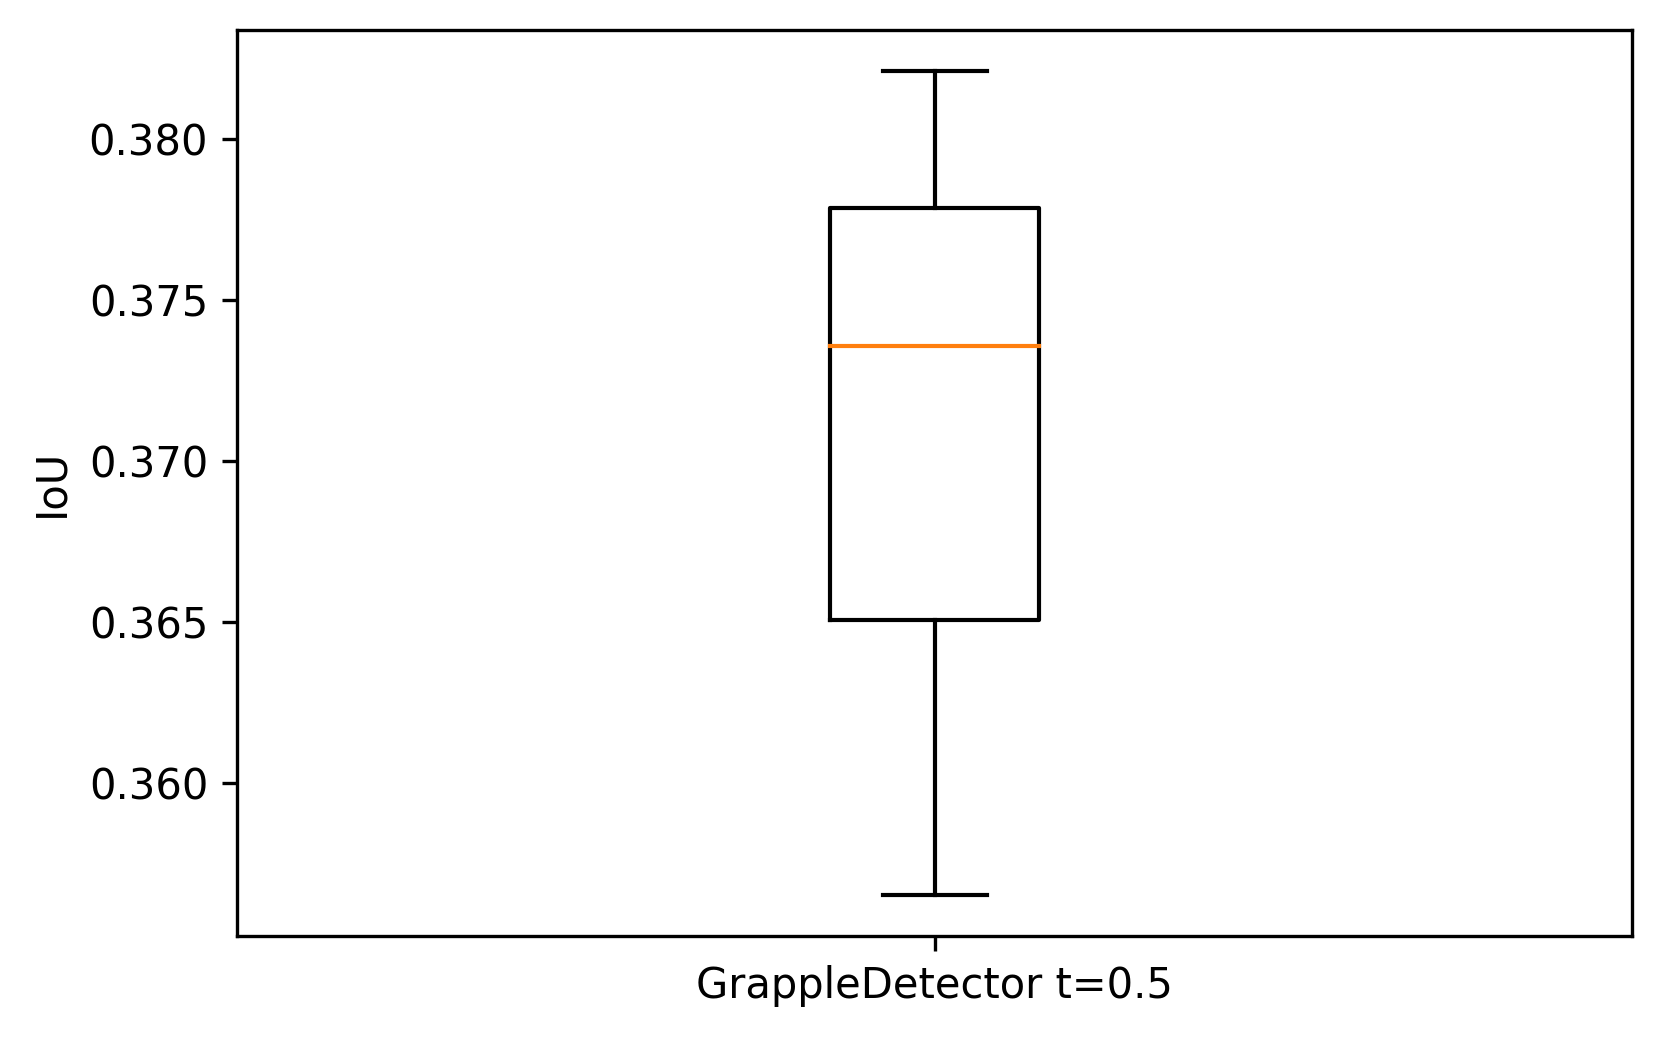
\includegraphics[width=1\textwidth,center]{bilder/Hauptteil/Autoencoder_Grappel_Detection/IoU_05_AE_Grapple.png}
    		\caption{Schwellenwert 0.5}
    		\label{img:BoxPlot_RegressionAufAutoencoder05}	
    	\end{subfigure}
    	\centering
    \begin{subfigure}[c]{0.29\textwidth}			
    	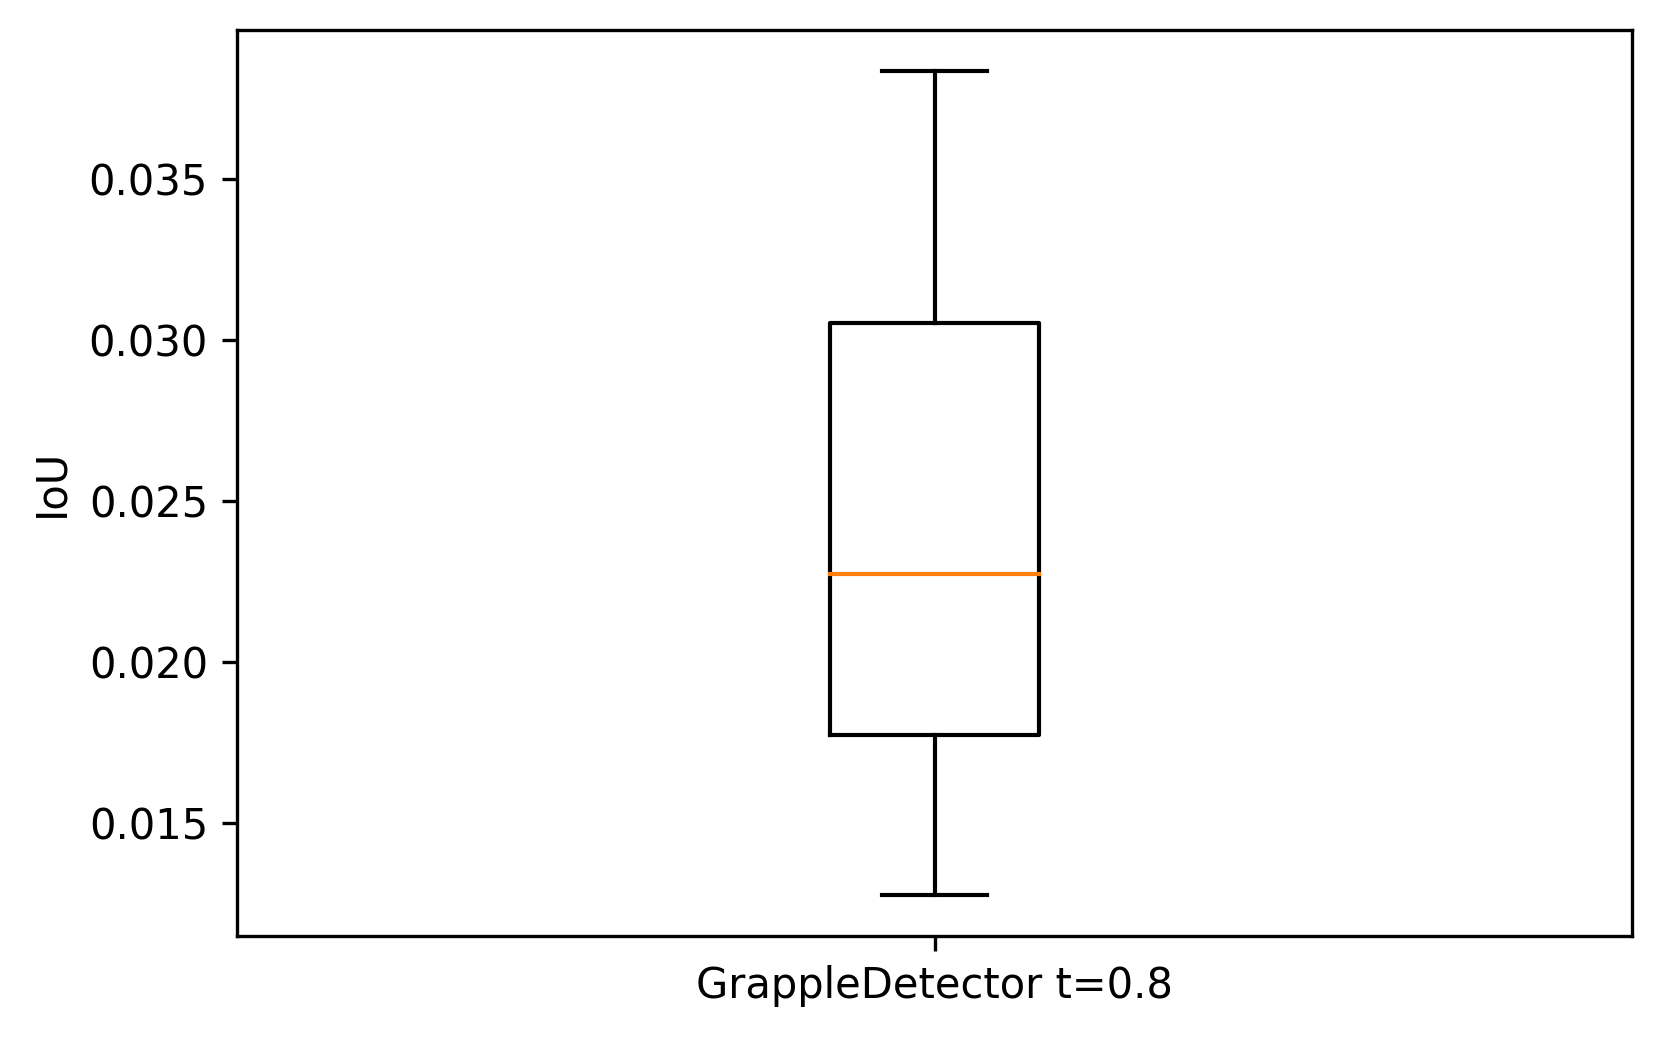
\includegraphics[width=1\textwidth,center]{bilder/Hauptteil/Autoencoder_Grappel_Detection/IoU_08_AE_Grapple.png}
    	\caption{Schwellenwert 0.8}
    	\label{img:BoxPlot_RegressionAufAutoencoder08}	
    \end{subfigure}
    	\begin{subfigure}[c]{0.29\textwidth}			
    		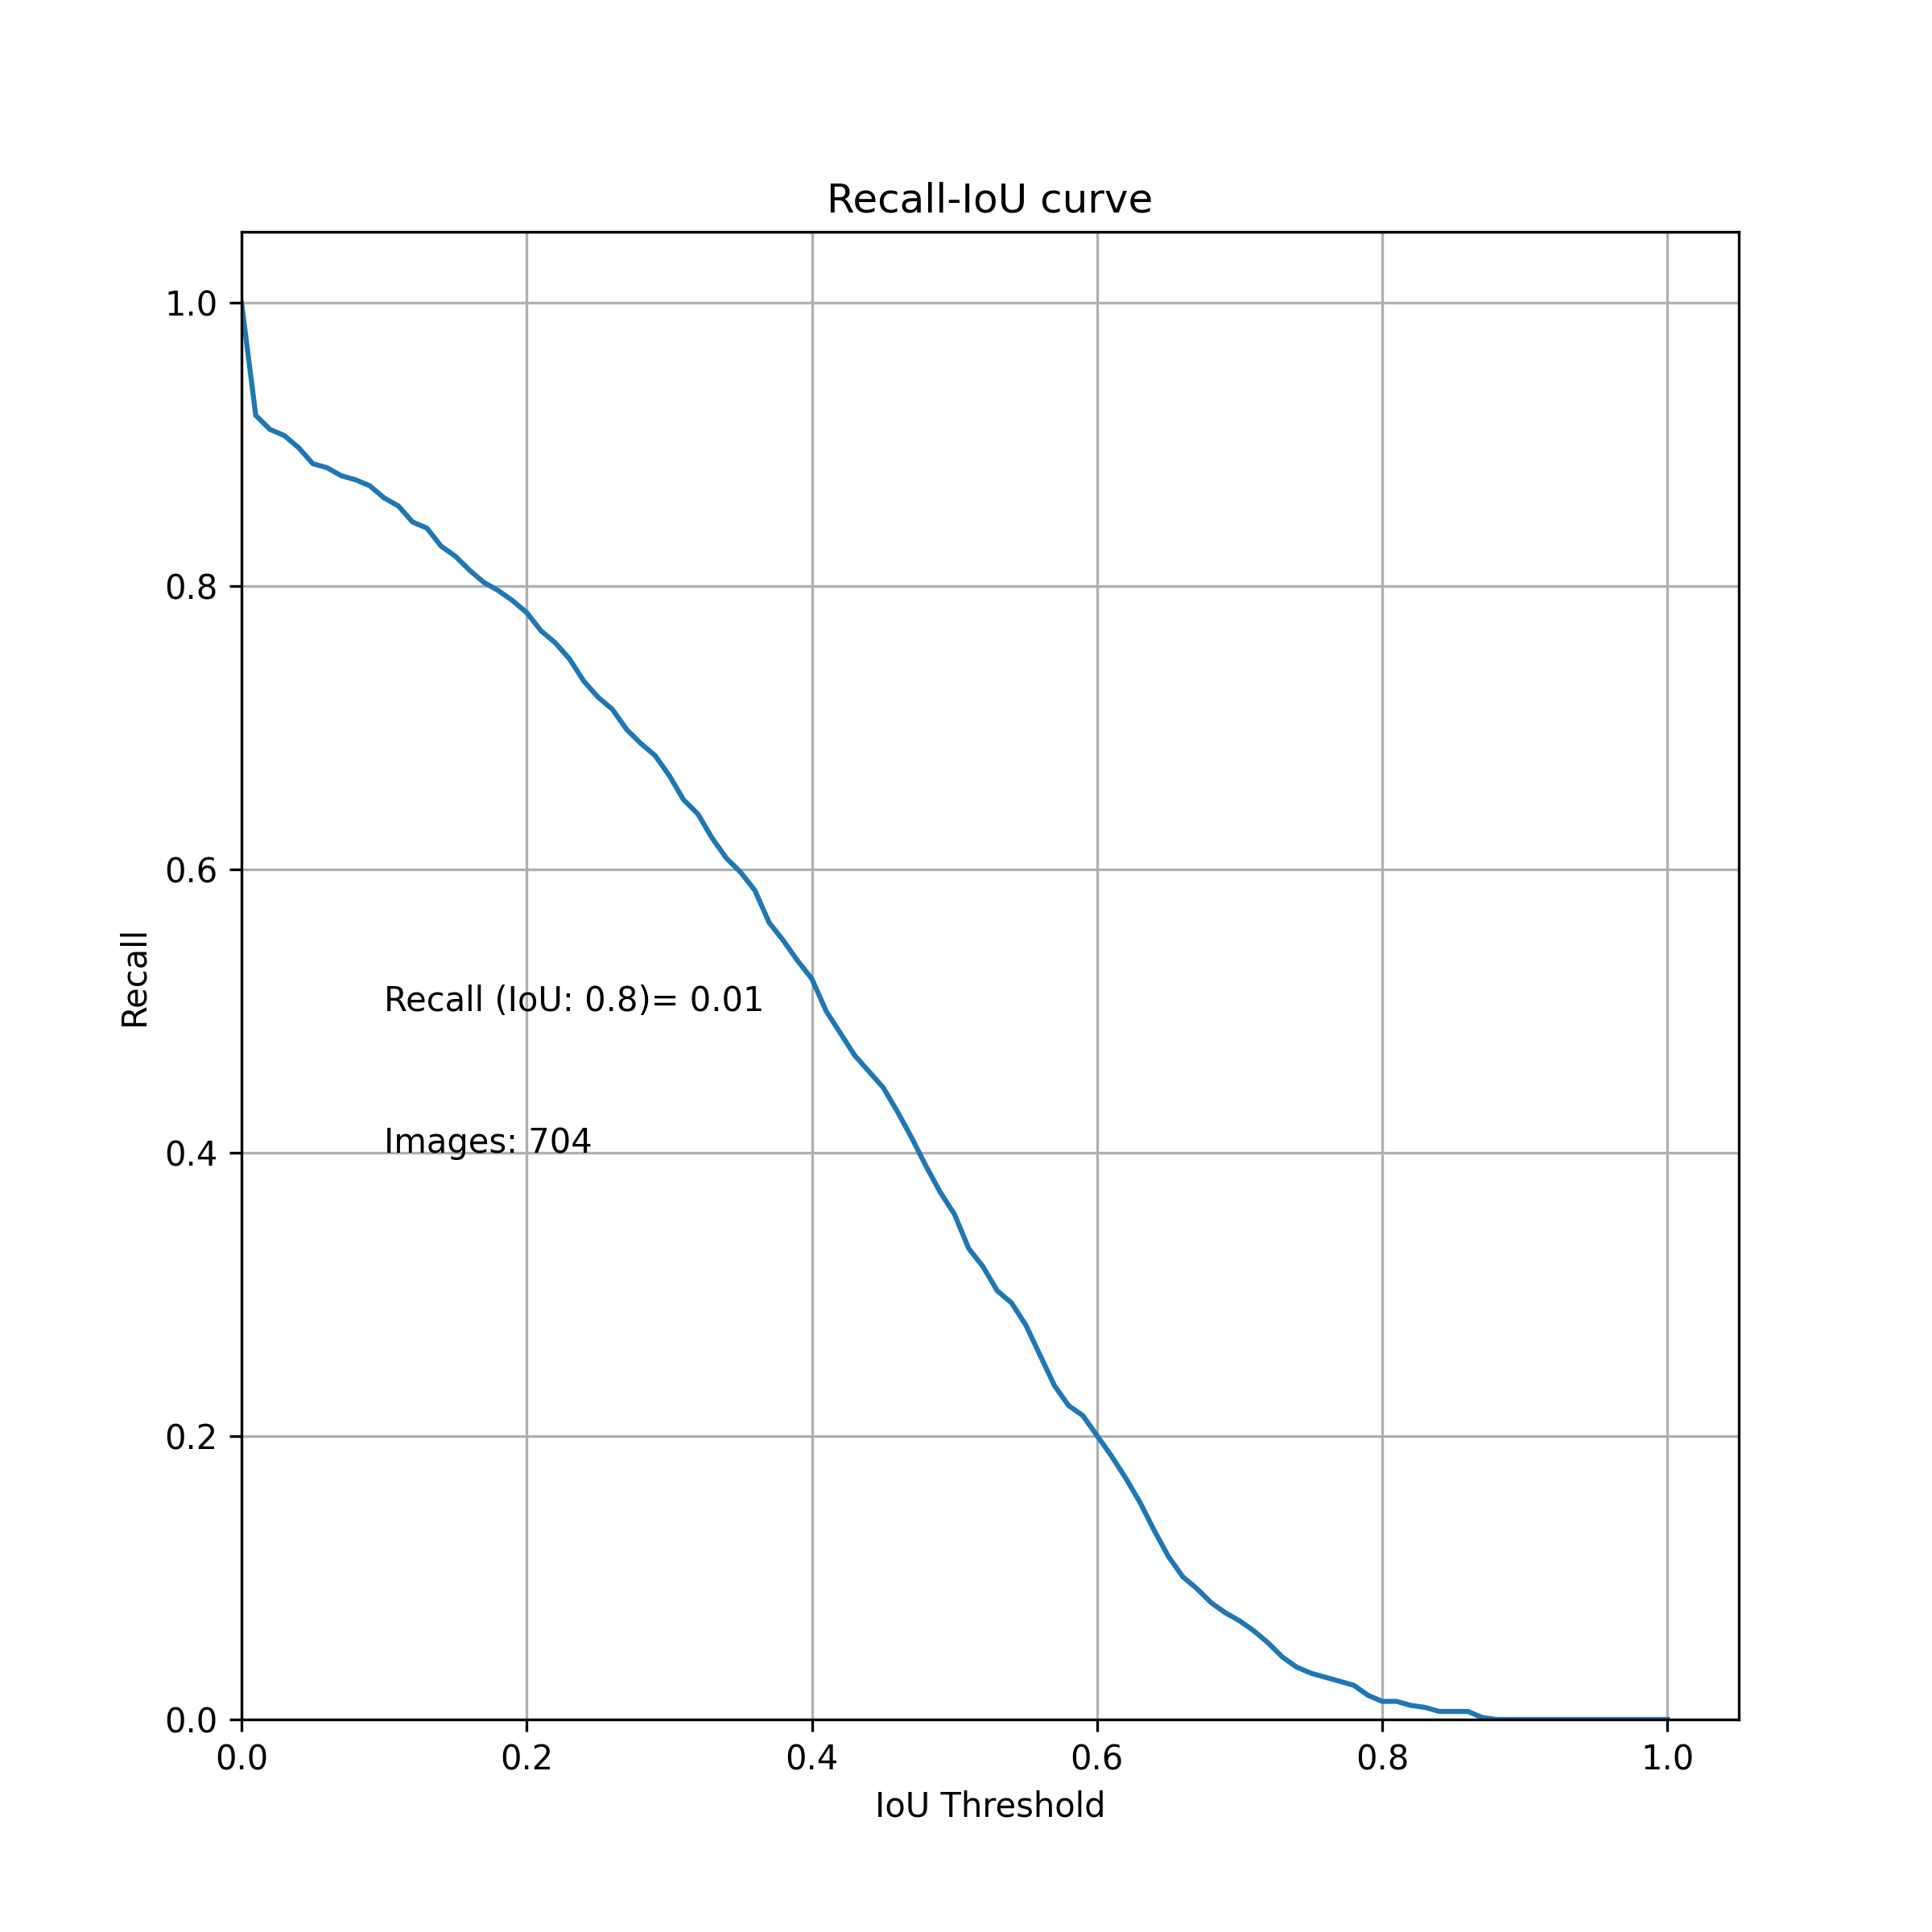
\includegraphics[width=1\textwidth, center]{bilder/Hauptteil/Autoencoder_Grappel_Detection/IoU.png}
    		\caption{Recall-IoU-Curve}
    		\label{img:RecalllIoUt_RegressionAufAutoencoder}	
    	\end{subfigure}
    	\caption{Ergebnis Regression auf Autoencoder}
        \label{img:ErgebnissRegressionAufAE}
    \end{figure}
 

%	  \begin{figure}[h]
%		\centering
%		\begin{subfigure}[c]{0.49\textwidth}			
%			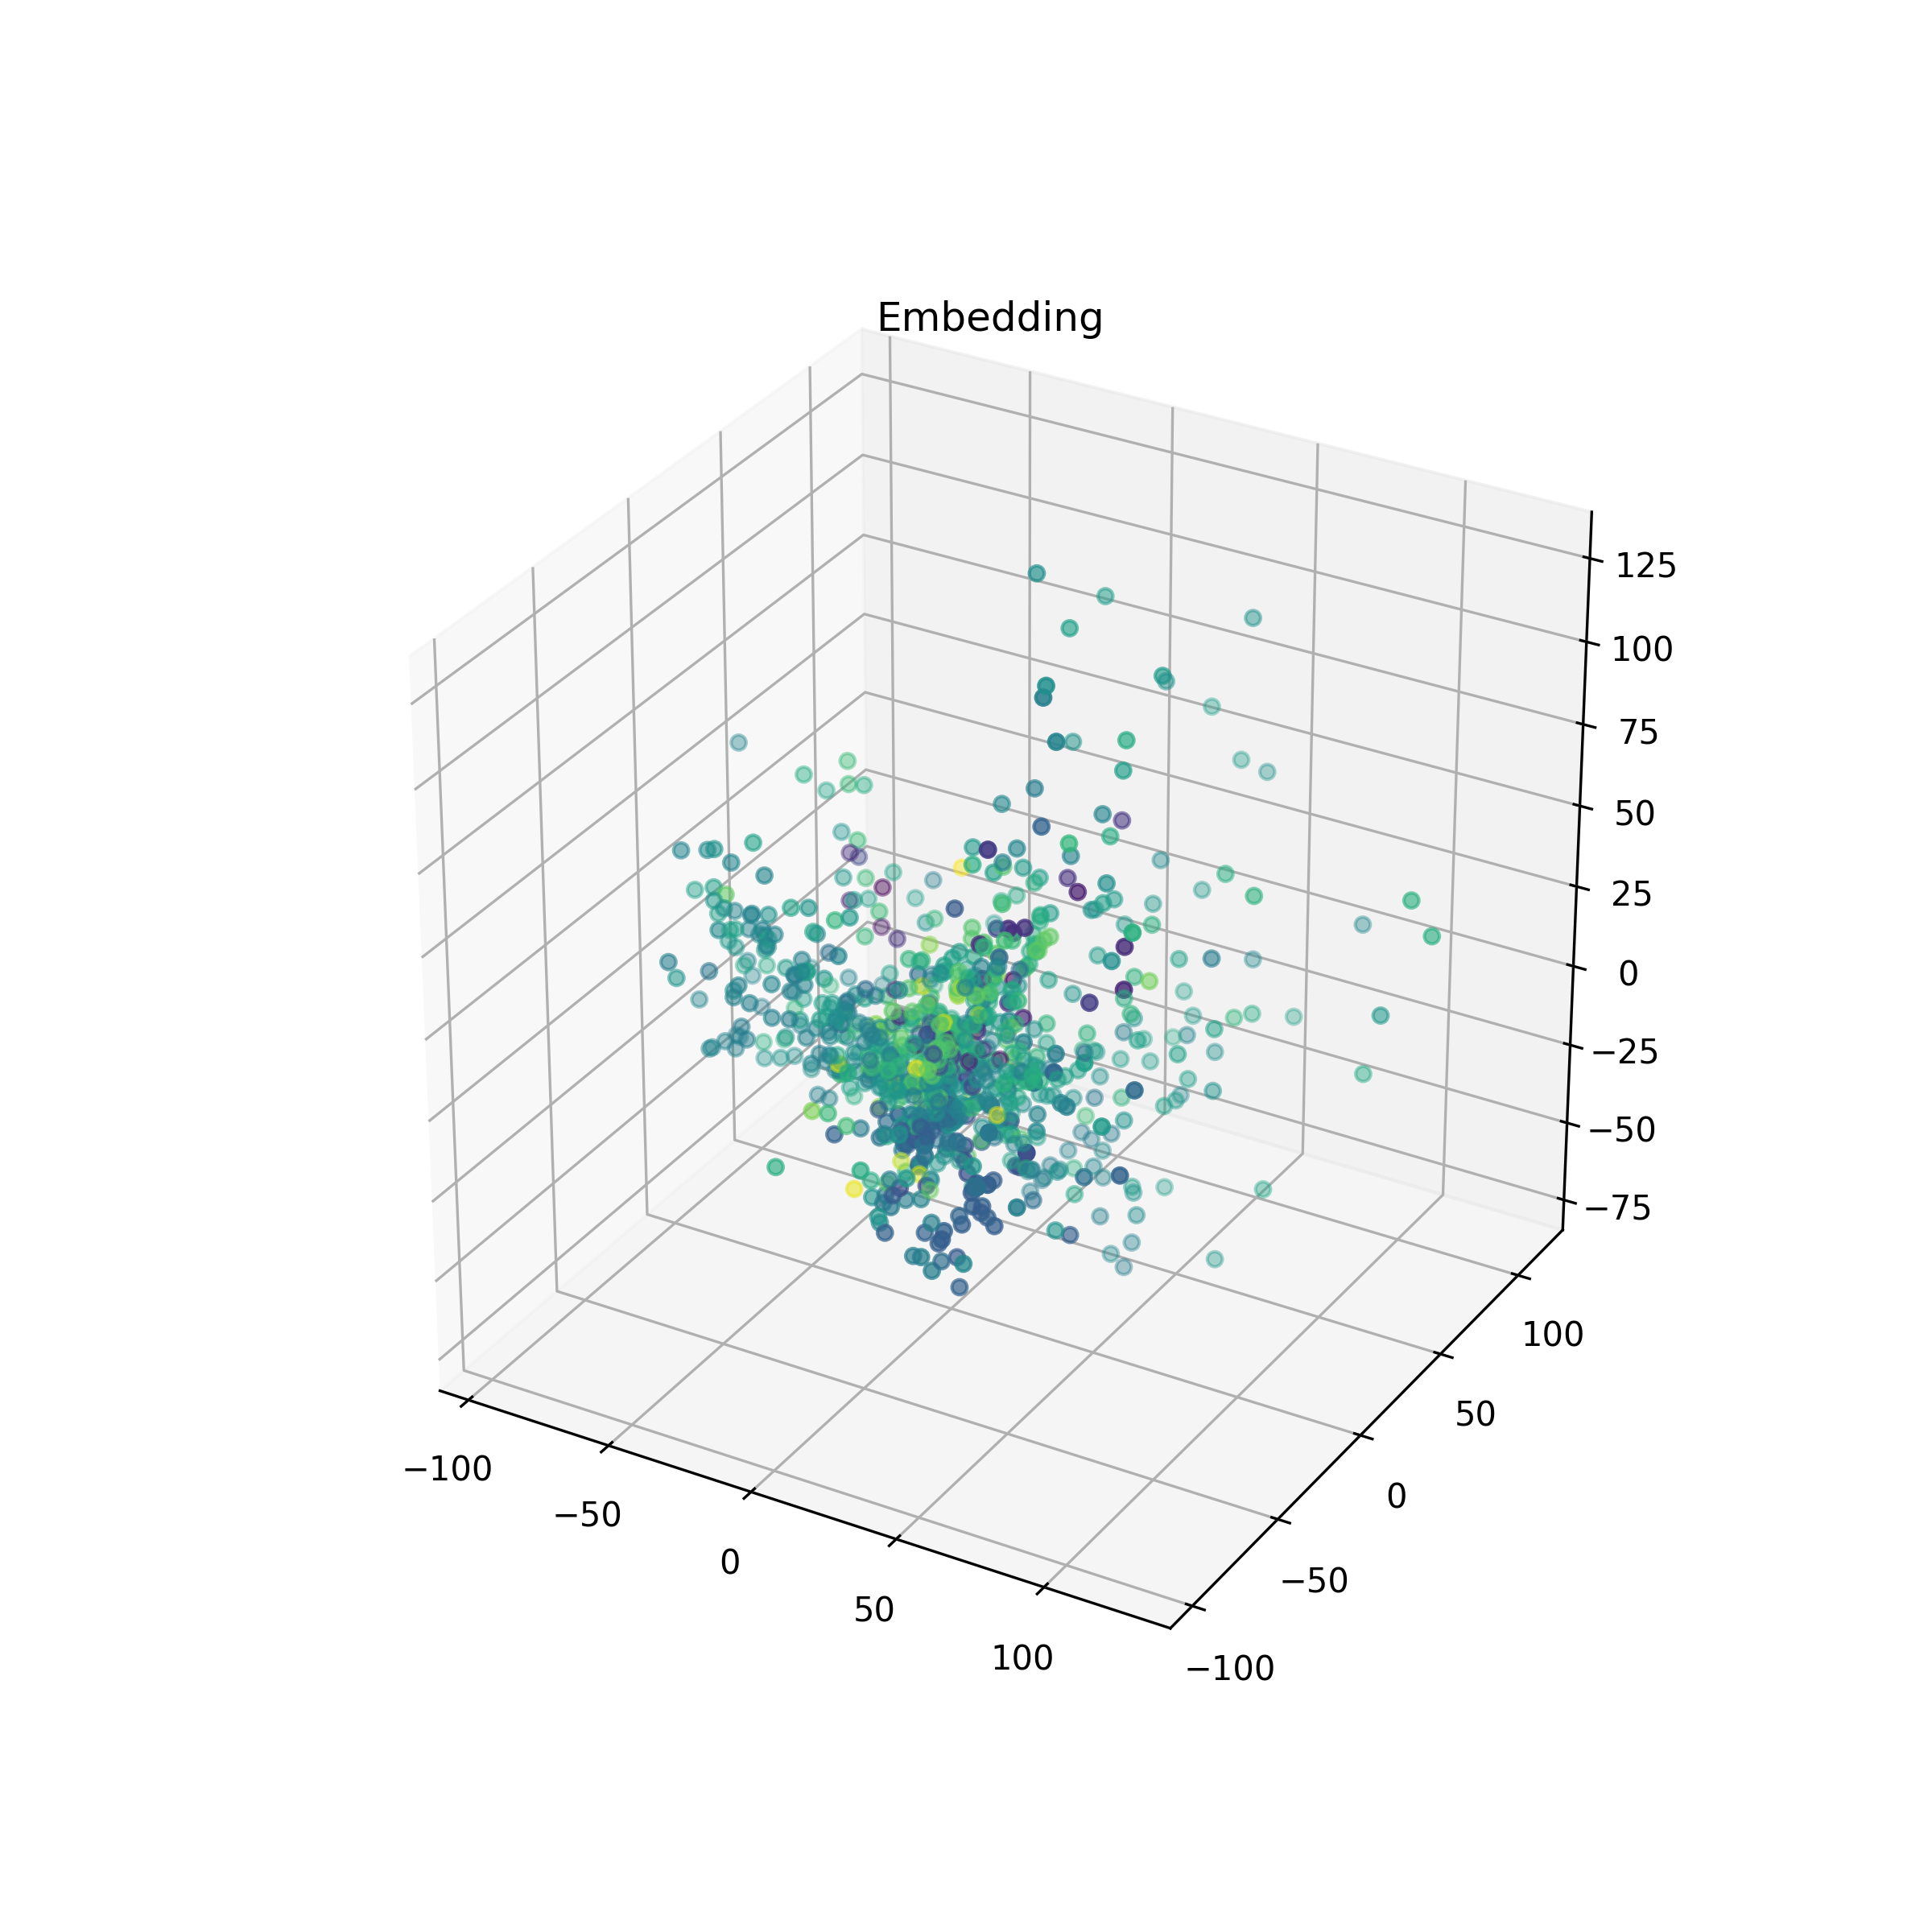
\includegraphics[width=1\textwidth,center]{bilder/Hauptteil/Autoencoder_Grappel_Detection/Embedding_y.png}
%			\caption{Embedding mit y-Psoition des Greifers}
%			\label{img:BoxPlot_RegressionAufAutoencoder}	
%		\end{subfigure}
%		\begin{subfigure}[c]{0.49\textwidth}			
%			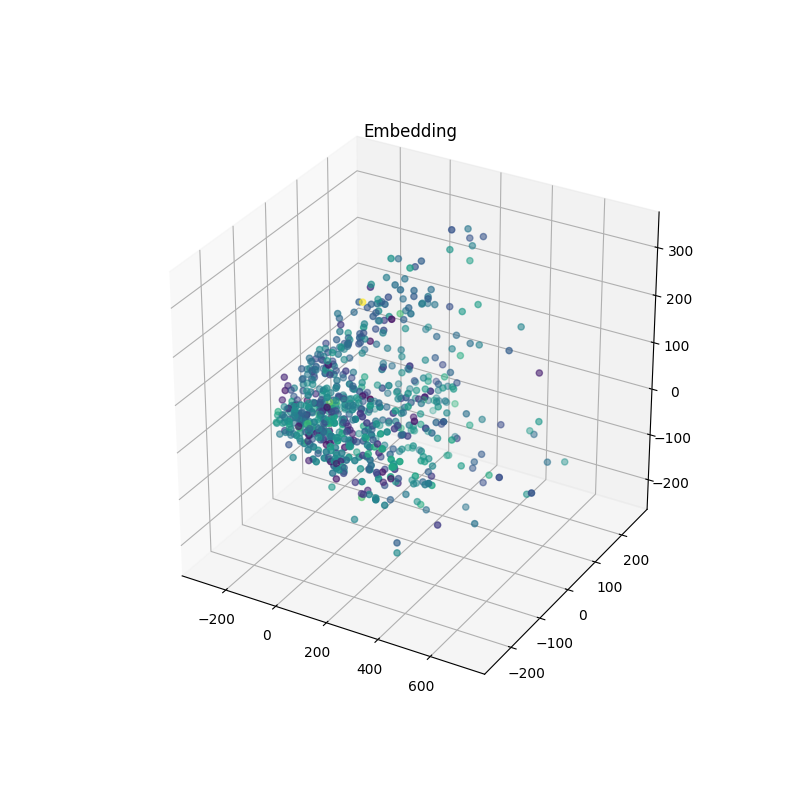
\includegraphics[width=1\textwidth, center]{bilder/Hauptteil/Autoencoder_Grappel_Detection/Embedding_x.png}
%			\caption{Embedding mit x-Psoition des Greifers}
%			\label{img:RecalllIoUt_RegressionAufAutoencoder}	
%		\end{subfigure}
%		\caption{Embedding Autoencoder}
%		\label{img:EmbeddingAE_M}
%	\end{figure}
	
	\todo{Bilder Einbettung auswählen}
	  \begin{figure}[h]
		\centering
		\begin{subfigure}[c]{0.49\textwidth}			
			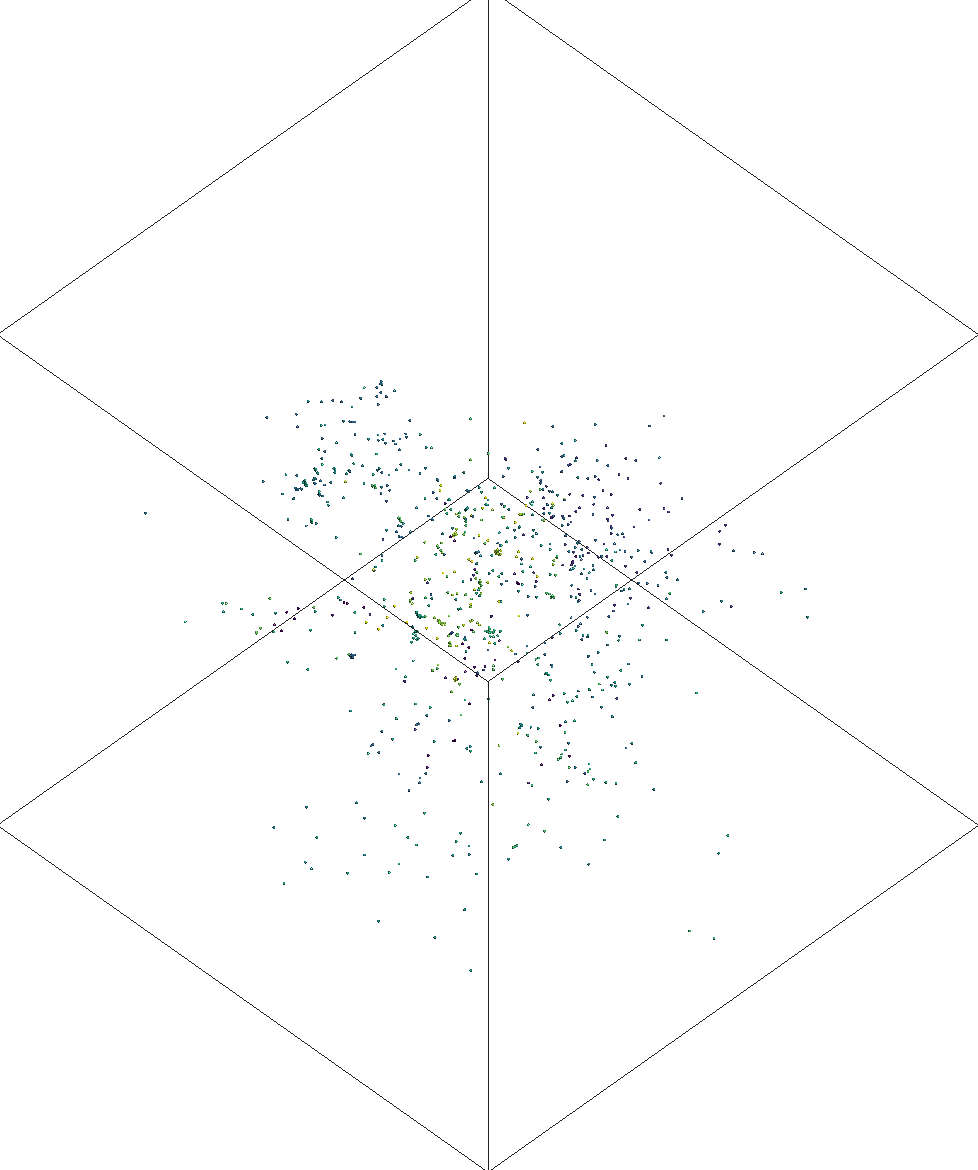
\includegraphics[width=1\textwidth,center]{bilder/Hauptteil/Autoencoder_Grappel_Detection/y_embKopie.png}
			\caption{Embedding mit y-Position des Greifers}
			\label{img:Emb_y_AE}	
		\end{subfigure}
		\begin{subfigure}[c]{0.49\textwidth}			
			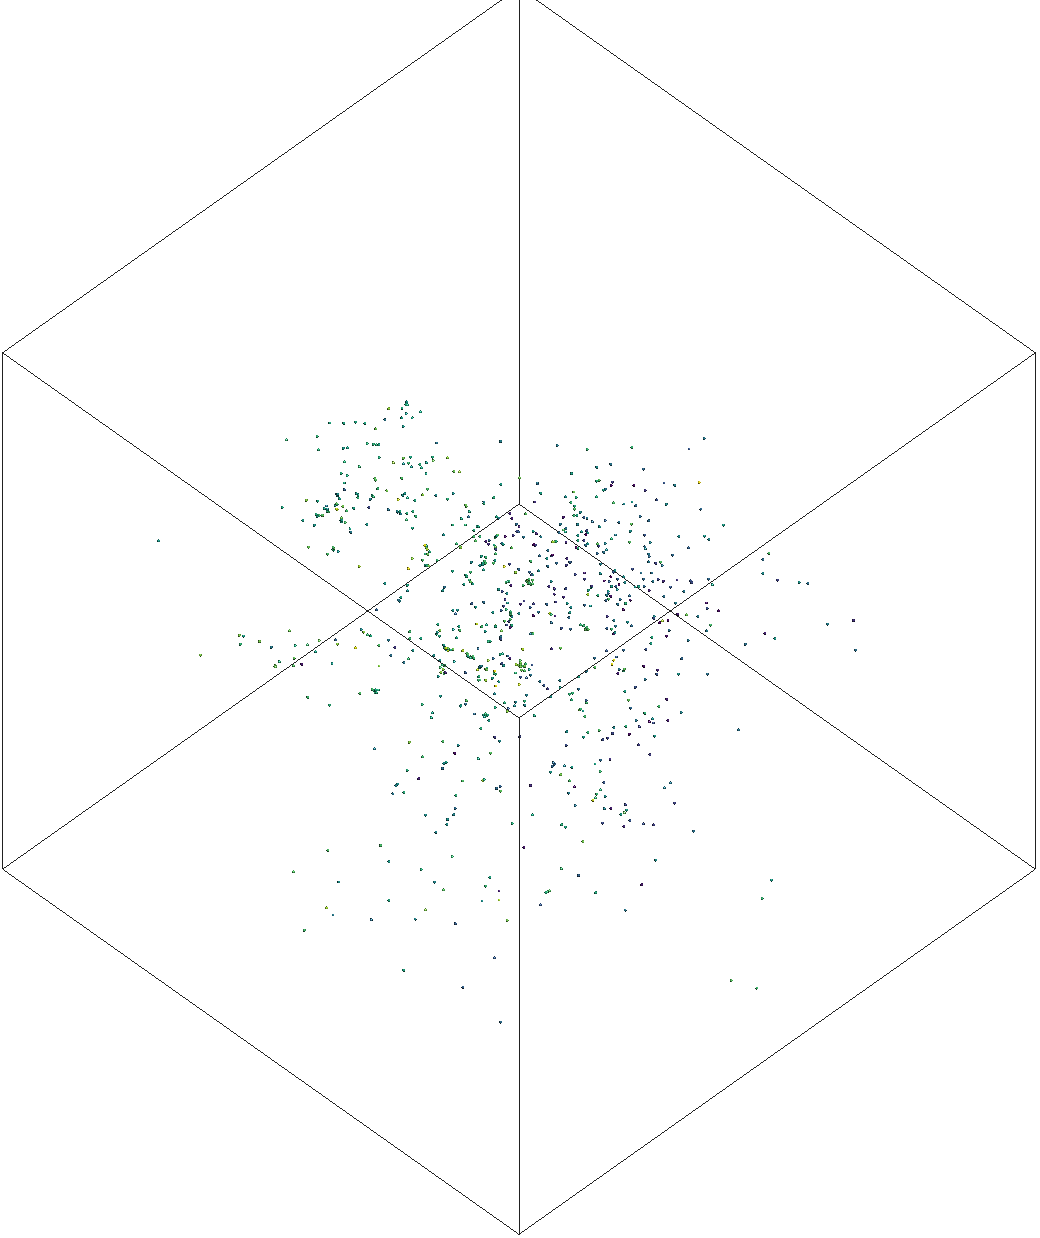
\includegraphics[width=1\textwidth, center]{bilder/Hauptteil/Autoencoder_Grappel_Detection/x_embKopie.png}
			\caption{Embedding mit x-Position des Greifers}
			\label{img:Emb_x_AE}	
		\end{subfigure}
		\caption{Embedding Autoencoder}
		\label{img:EmbeddingAE_V}
	\end{figure}
	
	\begin{figure}[h]
		\centering
		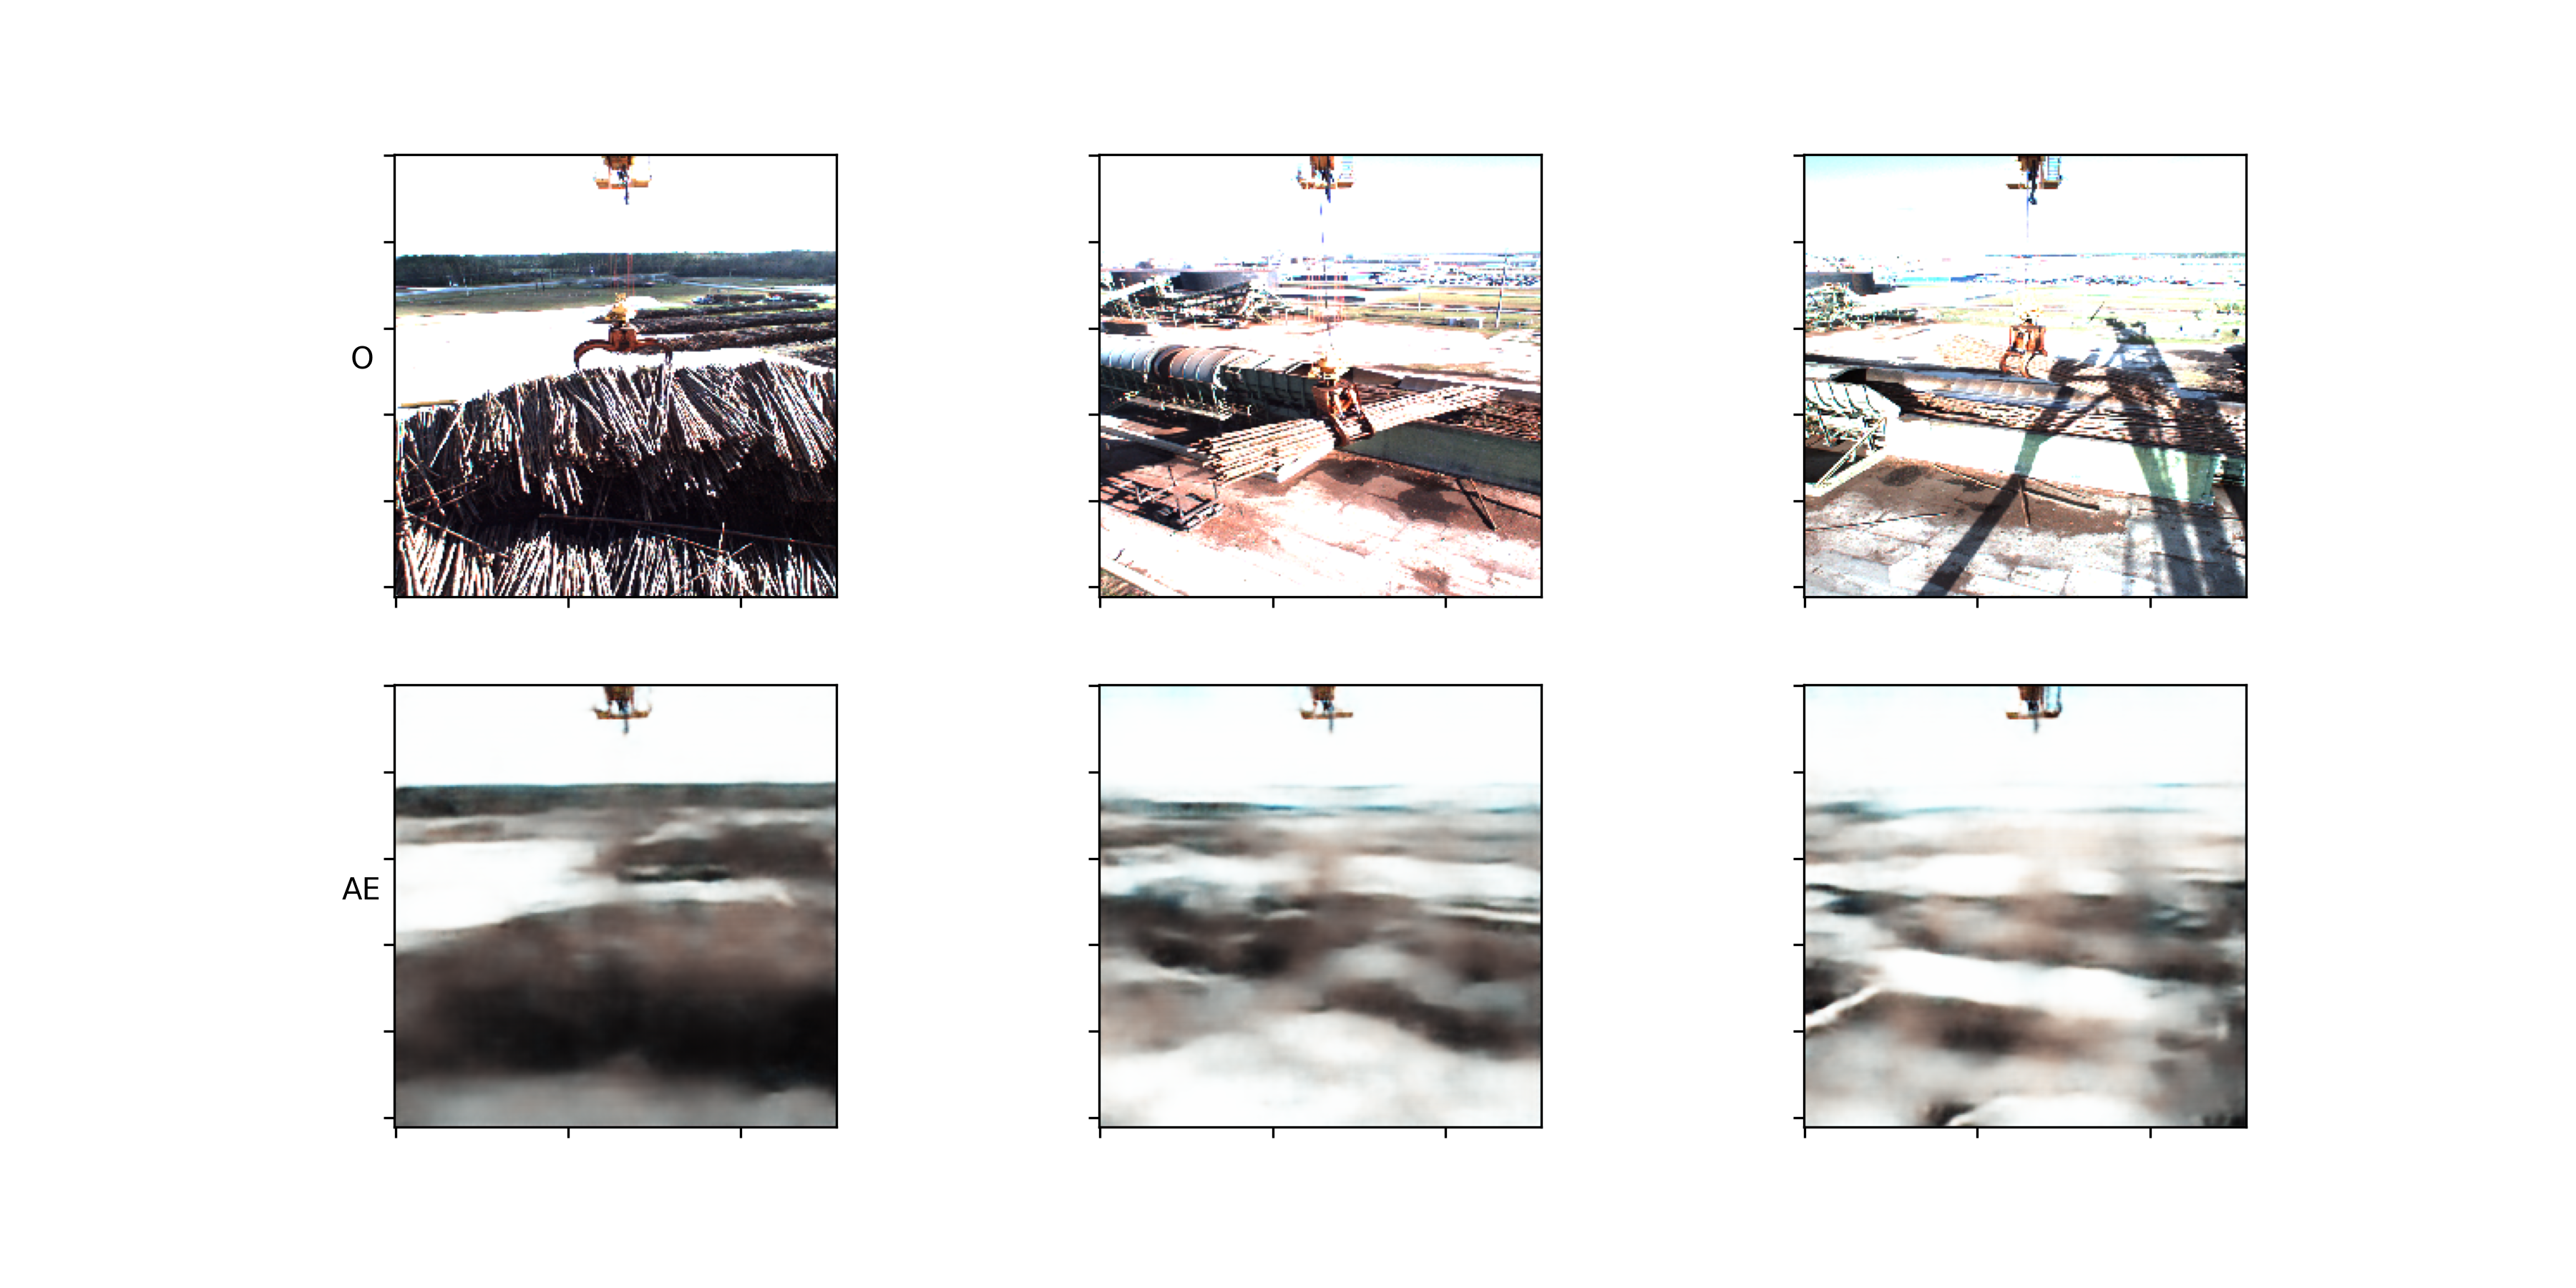
\includegraphics[width=1\textwidth, center]{bilder/Hauptteil/Autoencoder_Grappel_Detection/OriginalPicturesAndReconstruction.png}
		\caption{Rekonstruktion Autoencoder}
		\label{img:RekonstruktionAE}
	\end{figure}  
	
	
	
	\section{Aufgabenfokussierung und Greifererkennung}
	\label{sec:MultiTaskGreifererkennung}
	Im Ansatz \ref{sec:GreifererkennungAufAutoencoder} wurde die fehlende Fokussierung des Autoencoders auf den Greifer als Schwäche ausgemacht. Als neuer Ansatz wird untersucht, ob ein gleichzeitiges Lernen der Datenrepräsentation und das finden des Rahmens um den Greifer, den Autoencoder fokussiert und gleichzeitig gute Ergebnisse für die Regression gefunden werden können. Konkret wird ein \ac{simo} Ansatz untersucht.  
	
	\subsection{Werkzeug: TaskFocusingOnAutoencoder}
	\label{subsec:SecondCriterionAutoenocder}
	Zur Umsetzung des Ansatzes wurde ein Modul in Python erstellt. Da eine Aufgabe des Multi-Task-Ansatzes ein Autoencoder ist, wurde als Basis die Klasse ConvolutionalAutoencoder des Moduls autoencoder.py genutzt. Es wurde ein neues Modul erstellt, welches zusätzlich zu der Rekonstruktion des Autoencoders einen weiteren Ausgang bereitstellt. Der weitere Ausgang kann, wie jeder Ausgang für eine Binärklassifikation, für eine Multiklassifikation, für eine Regression oder jede andere beliebige Aufgabe genutzt werden. In Abbildung \ref{img:SchemaTFAE} ist der schematische Aufbau des Ansatzes abgebildet. Die Schichten des weiteren Kriteriums werden an die Code-Schicht des Autoencoders angehängt. Es können beliebig viele Schichten genutzt werden. Die Verlustfunktion des neuronalen Netzwerkes besteht aus der Summe der einzelnen Verlustfunktionen und einer Gewichtung. Sie lautet im Detail: 
	\begin{align}
	loss = weight1 * loss\_autoencoder + weight2 * loss\_task2
	\end{align}
	Die Gewichtung der Verlustfunktionen wird per Konstruktor-Argument übergeben. In Abbildung \ref{img:KlassendiagrammTFAE} ist das Klassendiagramm des TaskFocusingOnAutoencoder kurz TFAE dargestellt.
	\begin{figure}[h]
		\centering
		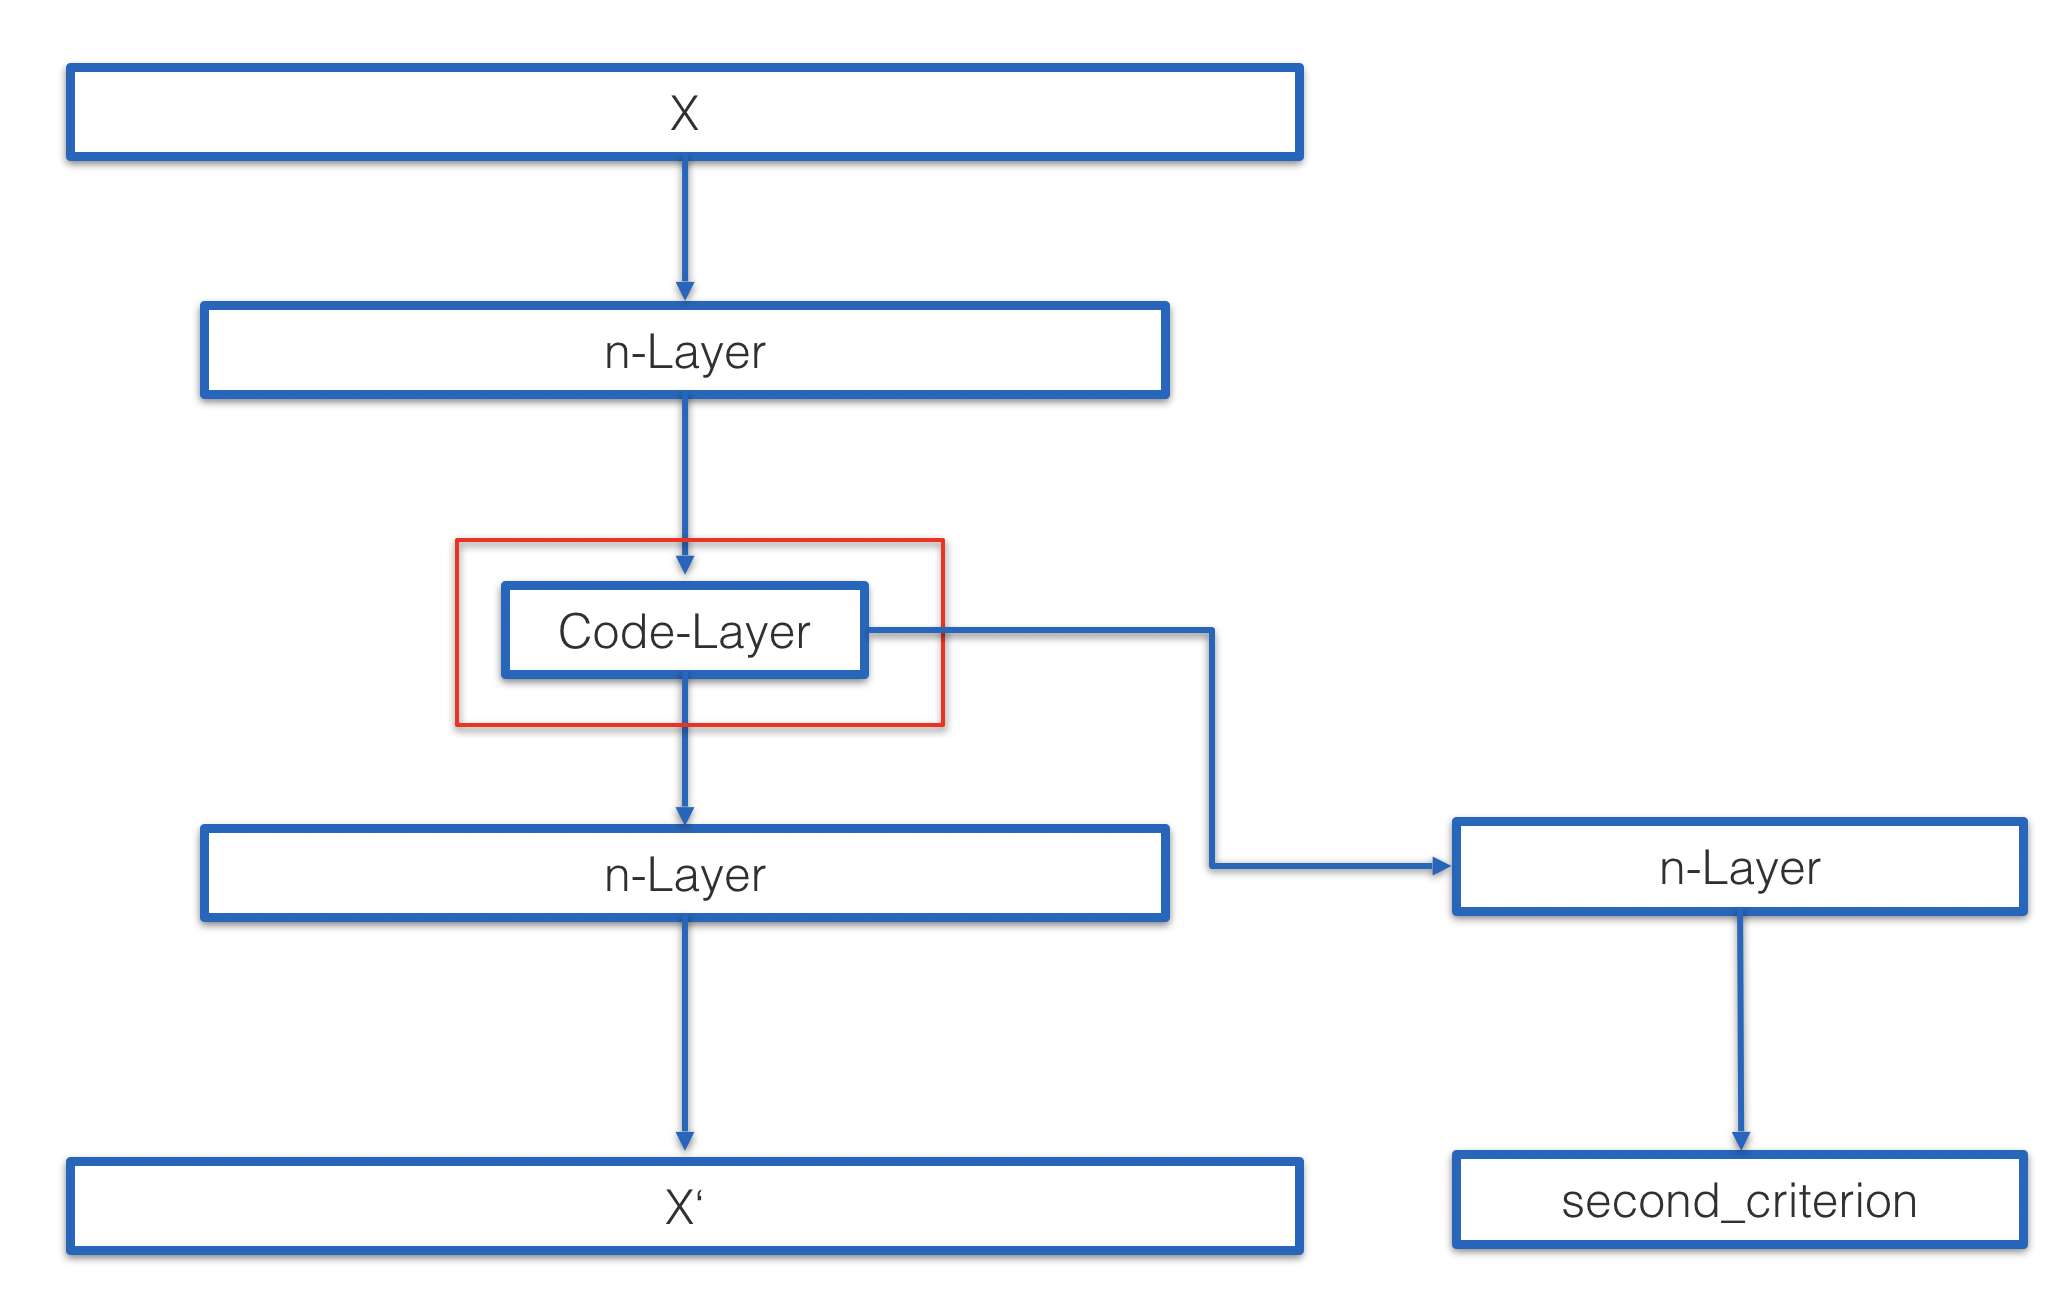
\includegraphics[width=0.7\textwidth, center]{bilder/Schema_Autoencoders/Schema_SCAE.png}
		\caption[Schema TaskFocusingOnAutoencoder]{Schema TaskFocusingOnAutoencoder}
		\label{img:SchemaTFAE}
	\end{figure}  
	\begin{figure}[h]
		\centering
		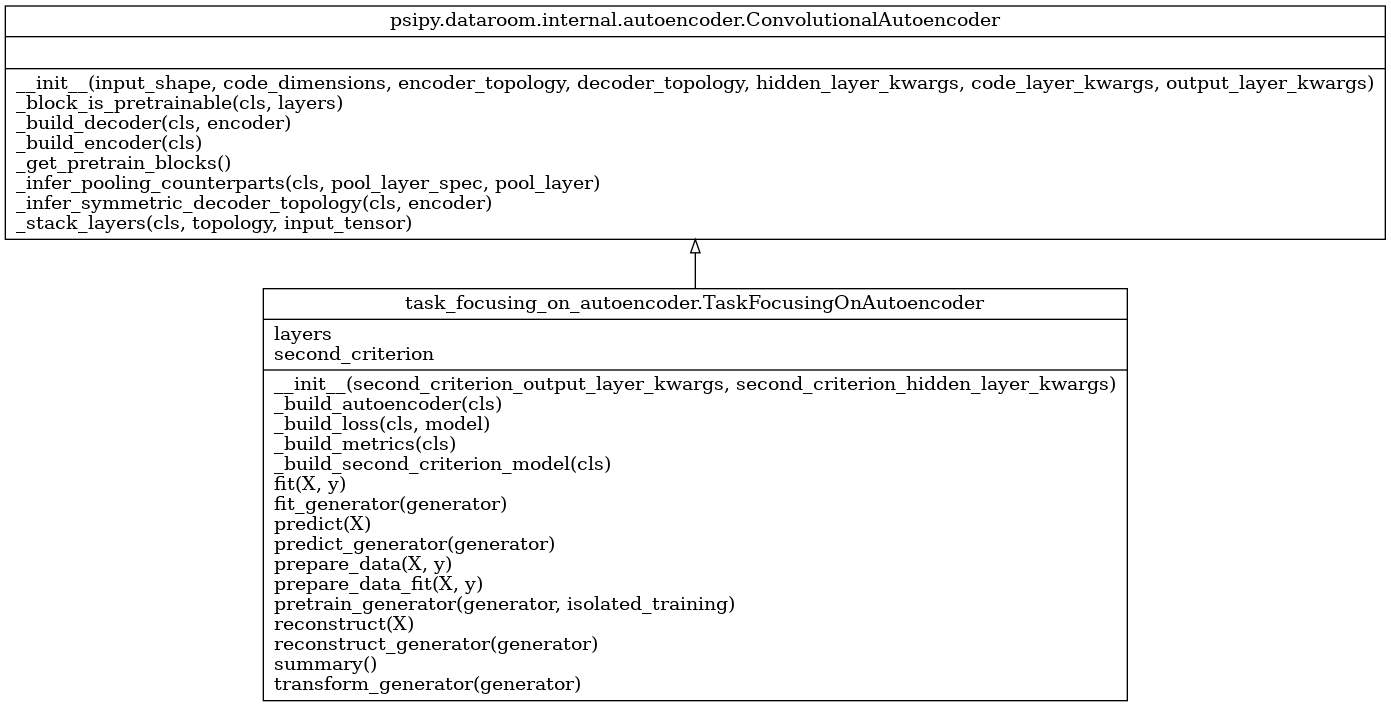
\includegraphics[width=0.7\textwidth, center]{bilder/Klassendiagramme/TFAE.png}
		\caption[Klassendiagramm TaskFocusingOnAutoencoder]{Klassendiagramm TaskFocusingOnAutoencoder}
		\label{img:KlassendiagrammTFAE}
	\end{figure}  
	Über den Konstruktor können alle Argumente, welche zum Erstellen des Models notwendig sind, per doppeltes Sternchen Wörterbuch Argument (**kwargs) an die Klasse übergeben werden. Diese Technik erlaubt es, eine mit Schlüsselwörtern versehene Argumentliste variabler Länge zu übergeben. Die Argumentlisten werden beinahe in allen Methoden zum Einsatz gebracht. Sie werden insbesondere genutzt, um Argumente an die zugehörigen Keras-Methoden zu übergeben. Die Namensgebung der Methode orientiert sich dabei an Keras. So wird z. B. in dem Methodenaufruf $fit(..)$ unter anderem auch die Keras-Methode $fit(..)$ aufgerufen. Um einen TFAE zu trainieren, ist es notwendig eine Instanz zu erzeugen, die Methode $pretrain(..)$ aufzurufen und ihn anschließend mit der Methode $fit(..)$ zu trainieren.
	In dem Methodenaufruf $pretrain(..)$ wird das Modell erstellt und schichtenweise vortrainiert. Das eigentliche Training erfolgt in der Methode $fit(..)$. Alternativ können auch die zugehörigen Generatorenklassen aufgerufen werden.    

	In Listing \ref{lst:BspErstellungConvolutionalSecondCriterionAutoenocder} ist beispielhaft dargestellt, wie ein TFAE erstellt wird. In den ersten 10 Zeilen wird die Architektur erstellt. Ab Zeile 12 wird eine Instanz eines TFAE mittels Argumentenliste erstellt. Zu beachten ist, dass hier keine Decoder-Architektur übergeben wird. Wenn keine Decoder-Architektur bereitgestellt wird, wird sie beim Erstellen des eigentlichen Modells aus der Encoder-Architektur abgeleitet.
	\begin{lstlisting}[language=python,caption=Beispiel Erstellung ConvolutionalSecondCriterionAutoenocder in Python, label=lst:BspErstellungConvolutionalSecondCriterionAutoenocder]
	encoder_topology = [("Conv2D", {"filters": 8, "kernel_size": (3, 3)}),
	("Conv2D", {"filters": 8, "kernel_size": (3, 3)}),
	('MaxPooling2D', {"pool_size": (2, 2)}),
	("Conv2D", {"filters": 16, "kernel_size": (3, 3)}),
	("MaxPooling2D", {"pool_size": (2, 2)}),
	("Conv2D", {"filters": 16, "kernel_size": (3, 3)}),
	("Flatten", {}),
	("Dense", {"units": 16})]

	second_criterion_topology = [("Dense", {"units": num_classes}) ]

	tfae = TaskFocusingOnAutoencoder(
	input_shape=(28, 28, 1),	
	code_dimensions=3, 
	encoder_topology=encoder_topology,
	second_criterion_topology=second_criterion_topology,
	hidden_layer_kwargs = {'activation': 'relu'},
	output_layer_kwargs = {'activation': 'sigmoid'},
	second_criterion_hidden_layer_kwargs = {'activation': 'relu'},
	second_criterion_output_layer_kwargs = {'activation': 'softmax'},
	second_criterion_loss = 'categorical_crossentropy',
	loss_weights=[8., 1.],
	second_criterion_metrics = {'second_criterion':'accuracy'},
	code_layer_kwargs=dict())
	\end{lstlisting}
	Listing  \ref{lst:BspPretrainConvolutionalSecondCriterionAutoenocder}  zeigt den Aufruf der Methode Pretrain. Der Aufruf führt zu einem Schichtenweise-Trainieren des Netzwerkes mit den Daten x\_train bei 20 Epochen und einer Stapelgröße von 64. 
	\begin{lstlisting}[language=python,caption=Beispielaufruf Pretrain  in Python, label=lst:BspPretrainConvolutionalSecondCriterionAutoenocder]
	tfae.pretrain(x_train,epochs = 20, batch_size = 64)
	\end{lstlisting}

	Der Methodenaufruf $fit(..)$ funktioniert wie der $fit(..)$-Aufruf in Keras. In Zeile drei des Listing  \ref{lst:BspPretrainConvolutionalSecondCriterionAutoenocder}  ist zu erkennen, dass die Zielgrößen der verschiedenen Ausgänge einfach als Python-Wörterbuch übergeben werden können.
	\begin{lstlisting}[language=python,caption=Beispielaufruf Fit  in Python, label=lst:BspFitConvolutionalSecondCriterionAutoenocder]
	history = tfae.fit(
		x_train,
		{"decoder": x_train, "second_criterion": y_train}, 
		epochs=200,
		batch_size = 64,
		validation_data=(x_test,{"decoder": x_test, "second_criterion": y_test})
	)
	\end{lstlisting}

	\subsection{Ergebnis}
	
	\todo{Grapple-MT Ergebnisse einfügen}
	In Abbildung  xyz
	
	In der Repräsentation werden die Merkmale des Greifers deutlich abgebildet. .....Vergleicht man die Rekonstruktionen des ersten Ansatzes mit denen des TFAE lässt sich eine Fokussierung auf den Greifer erkennen. Besonders in Bild xyz zu sehen.
	
	
	
	\section{Transferlernen und 'Greifer beladen'-Klassifikation}
	\label{sec:TransferLearningGrappleLoaded}
	In vorangegangenen Kapitel wurde eine Repräsentation gefunden, welche die Merkmale des Greifer herausbildet. Ausgehend von dieser Repräsentation wird untersucht, ob ein Transfer auf weitere Aufgaben durchgeführt werden kann. Es wird der Ansatz des netzwerkbasierten tiefen Transferlernens genutzt um die Aufgabenstellung 'Greifer beladen' zu lösen.
	\subsection{Werkzeug: TaskTransferOnAutoencoder}
	\label{sec:TransferSecondCriterionAutoenocder}		
	Als Quelldomäne wird das Netzwerk, welches in Experiment \ref{sec:MultiTaskGreifererkennung} erstellt wurde genutzt. In der Zieldomäne werden die Architektur und die Gewichte des Auteoncoder weiterverwendet. Der zweite Task wird durch die Aufgabe der Klassifikation ob sich Baumstämme im Greifer befinden ersetzt. Abbildung \ref{img:SchemaTTAE} zeigt das Schema des Ansatzes. 
	\begin{figure}[h]
		\centering
		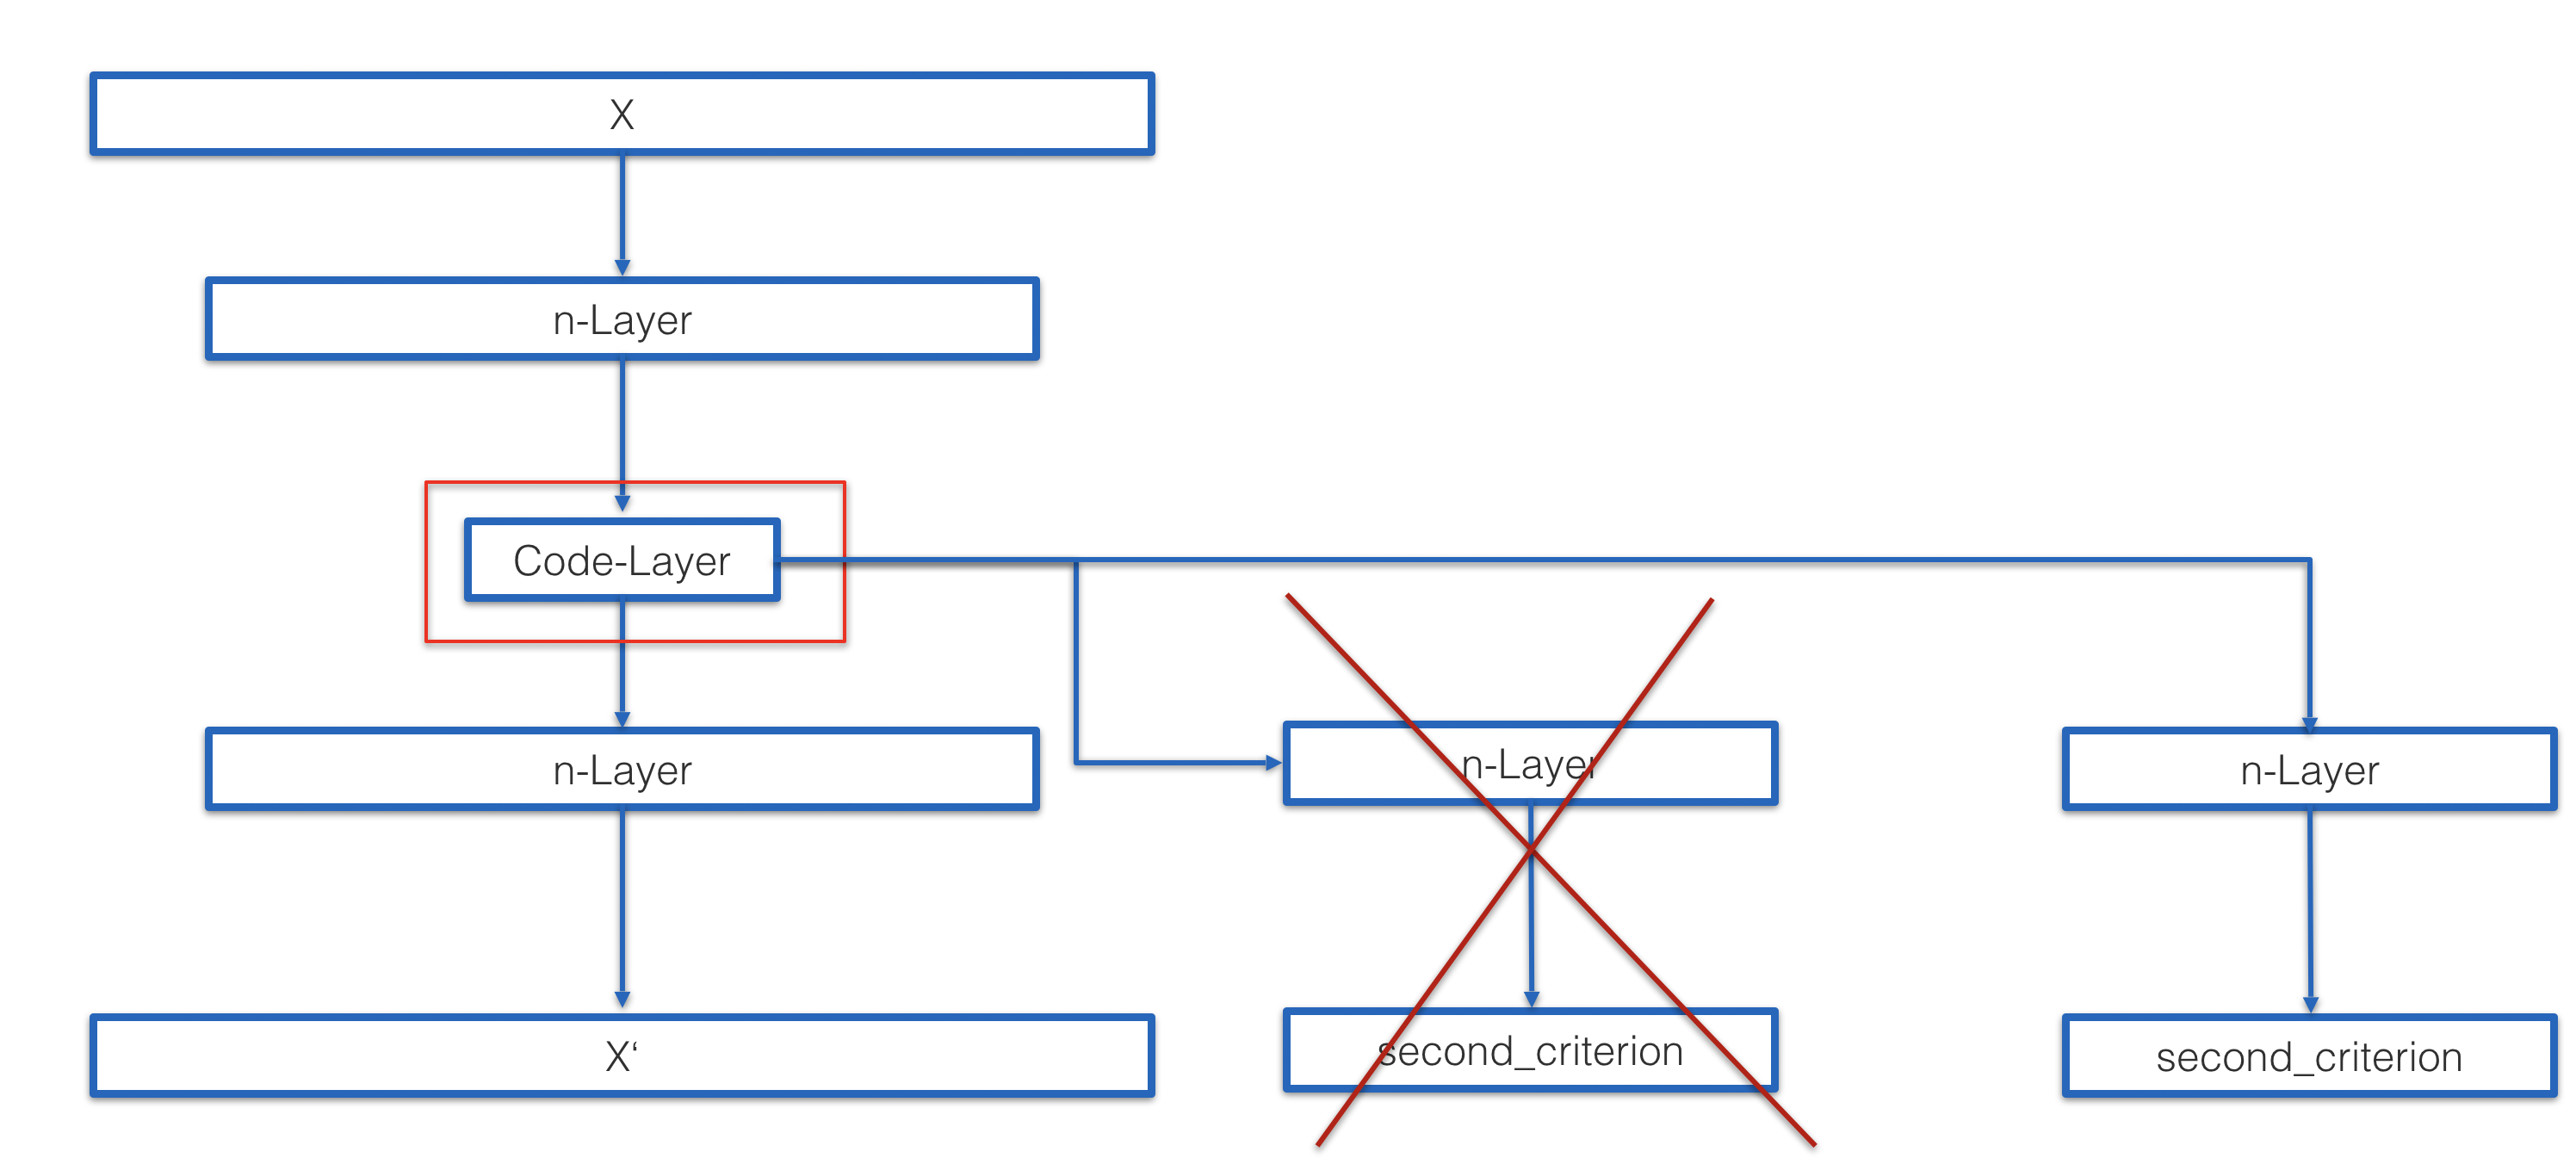
\includegraphics[width=0.5\textwidth, center]{bilder/Schema_Autoencoders/Schema_TSCAE.png}
		\caption[Schema TaskTransferOnAutoencoder]{Schema TaskTransferOnAutoencoder}
		\label{img:SchemaTTAE}
	\end{figure}
	Zur einfachen Anwendung des Ansatzes wurde ein Python-Modul mit der Klasse \acl{ttae} kurz \ac{ttae} erstellt. Abbildung \ref{img:KlassendiagrammTransferSecondCriterionAutoenocder} zeigt das zugehörige Klassendiagramm. Als Basis wird ein \ac{tfae} als Konstruktorargument übergeben. Die Parameter für den Autoencoder werden aus diesem Model kopiert. Zusätzlich müssen noch die Einstellungen für die zweite Aufgabe übergeben werden. Aus diesen beiden Teilen wird das neue Model erstellt. Die Parameter freeze\_encoder\_layers und freeze\_decoder\_layers ermöglichen es die Merkmalstransformation unverändert zu lassen. Es wird darüber gesteuert welche Schichten nicht neu trainiert werden können. 
	\begin{figure}[h]
		\centering
		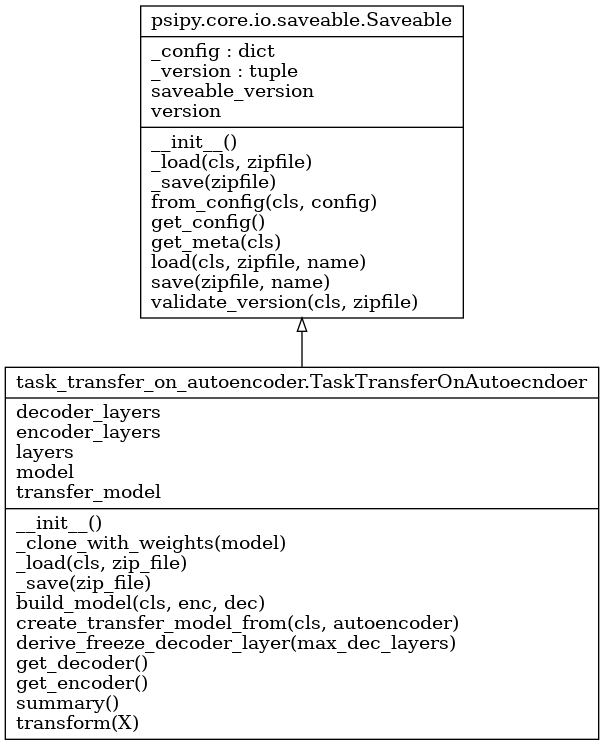
\includegraphics[width=0.5\textwidth, center]{bilder/Klassendiagramme/TTAE.png}
		\caption[Klassendiagramm TaskTransferOnAutoencoder]{Klassendiagramm TaskTransferOnAutoencoder}
		\label{img:KlassendiagrammTransferSecondCriterionAutoenocder}
	\end{figure}  
	Listing \ref{lst:BspTransferSecondCriterionAutoenocder} zeigt beispielhaft die Anwendung dieses Werkzeuges. Im Vergleich zu dem \ac{tfae} ist die Anwendung schon deutlich einfacher. Es gibt weniger Hyperparameter zum Modifizieren. Da das Modell auf einem trainierten \ac{tfae} basiert, ist kein $pretrain(..)$ mehr notwenig. Die Methode $fit(..)$ / $fit_generator(..)$ wird auf dieselbe Weise wie in Keras angewendet.	
	
	\begin{lstlisting}[language=python,caption=Beispiel TransferSecondCriterionAutoenocder in Python, label=lst:BspTransferSecondCriterionAutoenocder]
	tscm = TransferLearningConvolutionalSecondCriterionAutoencoder(csc_autoencoder,
	second_criterion_topology=second_criterion_topology,
	second_criterion_loss = 'binary_crossentropy',                                                                                                   
	second_criterion_hidden_layer_kwargs = {'activation': 'relu'},
	second_criterion_output_layer_kwargs = {'activation': 'sigmoid'}, 
	loss_weights=[1, 0.01],
	freeze_encoder_layers = 2
	,freeze_decoder_layers =[0,1])
	
	history = tscm.fit(
	x_train,
	{"decoder": x_train, "second_criterion": y_train}, 
	epochs=1,
	batch_size = 128,
	validation_data=(x_test,{"decoder": x_test, "second_criterion": y_test}))
	)
	\end{lstlisting}	
	
	\subsection{Ergebnis}
	Mit dem vorgestellten Ansatz lässt sich die Aufgabe 'Greifer beladen' lösen. Im Median von drei Versuchen wird ein Accuracy von 0.9827\% erreicht, was nahezu der Leistung der Basislinie mit einer Accuracy von 0.9828\% entspricht. In Abbildung \ref{img:Ergebnis_Transfer} sind die Ergebnisse des Versuchs dargestellt. Die Unterabbildung \ref{img:Einbettung_Logs_Vorhersage} stellt die neu gefundene Einbettung dar. Die blauen Datenpunte entsprechen der Vorhersage True Positiv, die lila Datenpunkte der Vorhersage True Negativ, gelb entspricht False Positiv und grün False Negativ. Es ist eine deutliche Anpassung der Einbettung an die Problemstellung erkennbar, wobei der Übergang von der einen zur anderen Klasse noch nicht 100\% korrekt ist.  

		 \begin{figure}[h]
			\centering
			\begin{subfigure}[c]{0.49\textwidth}			
				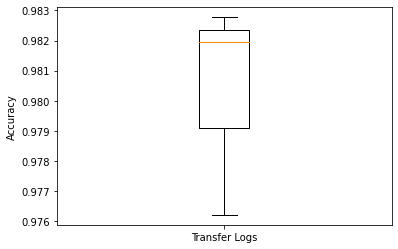
\includegraphics[width=1\textwidth,center]{bilder/Hauptteil/Transfer_Logs/Acc_Transfer_Logs.png}
				\caption{Accuracy}
				\label{img:AccuracyTransferLogs}	
			\end{subfigure}
			\begin{subfigure}[c]{0.49\textwidth}			
				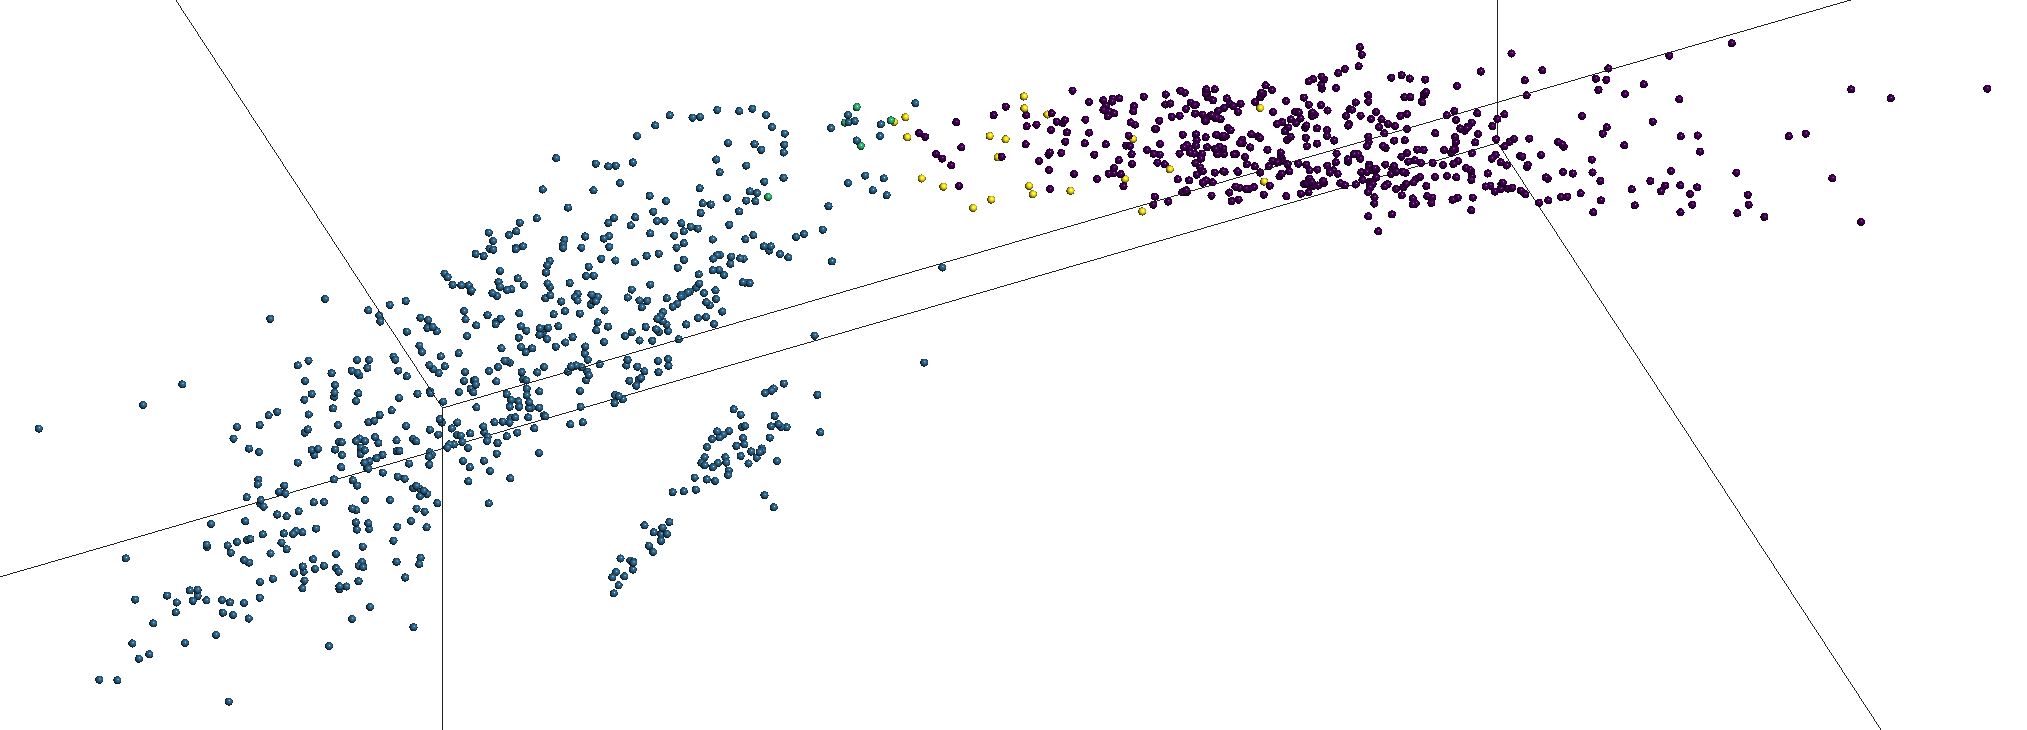
\includegraphics[width=1\textwidth, center]{bilder/Hauptteil/Transfer_Logs/Logs_transfer_emb.png}
				\caption{Einbettung mit Vorhersage}
				\label{img:Einbettung_Logs_Vorhersage}	
			\end{subfigure}
			\caption{Ergebnis Transfer}
			\label{img:Ergebnis_Transfer}
		\end{figure}
	
		
	\section{\ac{automl} und 'Greifer beladen'-Klassifikation}
	\label{sec:Transfer_autoMl}
	Die starke Anpassung an die Klassifikationsaufgabe im vorangegangenen Versuch motiviert einen Blick auf die Hyperparameter zur Gewichtung der Verlustfunktion zu werfen. Ziel dieses Versuches ist es, herauszufinden welchen Einfluss die Hyperparameter auf das Ergebnis hat. Es gibt sehr viele Möglichkeiten für die Gewichtung der Verlustfunktion. Um den manuellen Aufwand gering zu halten, wird ein neues Modul erstellt, welches auf \ac{automl} zur Hyperparameteroptimierung zurückgreift.
	\subsection{Werkzeug: AutoTaskTransferOnAutoencoder}
	\label{subsec:AutoTaskTransferOnAutoencoder}
	Das neue Modul integriert den Ansatz in der Klasse \acl{autottae}, kurz \ac{autottae}. Sie integriert die Klasse \acl{ttae} und erweitert sie mithilfe des HpBandSter-Frameworks um \ac{automl}-Ansätze zur \ac{hpo}. Konkret erbt die Klasse von hpbandster.core.worker. Zur Speicherung und Verwaltung der Hyperparameter wird auf die Klasse HyperparameterMixin zurückgegriffen. Nach nach dem Instanziieren der Klasse können weitere sinnvolle Hyperparameter gesetzt werden.
	In Abbildung \ref{img:KlassendiagrammAutoTaskTransferOnAutoencoder}  ist das zugehörige Klassendiagramm abgebildet. 
	\begin{figure}[h]
		\centering
		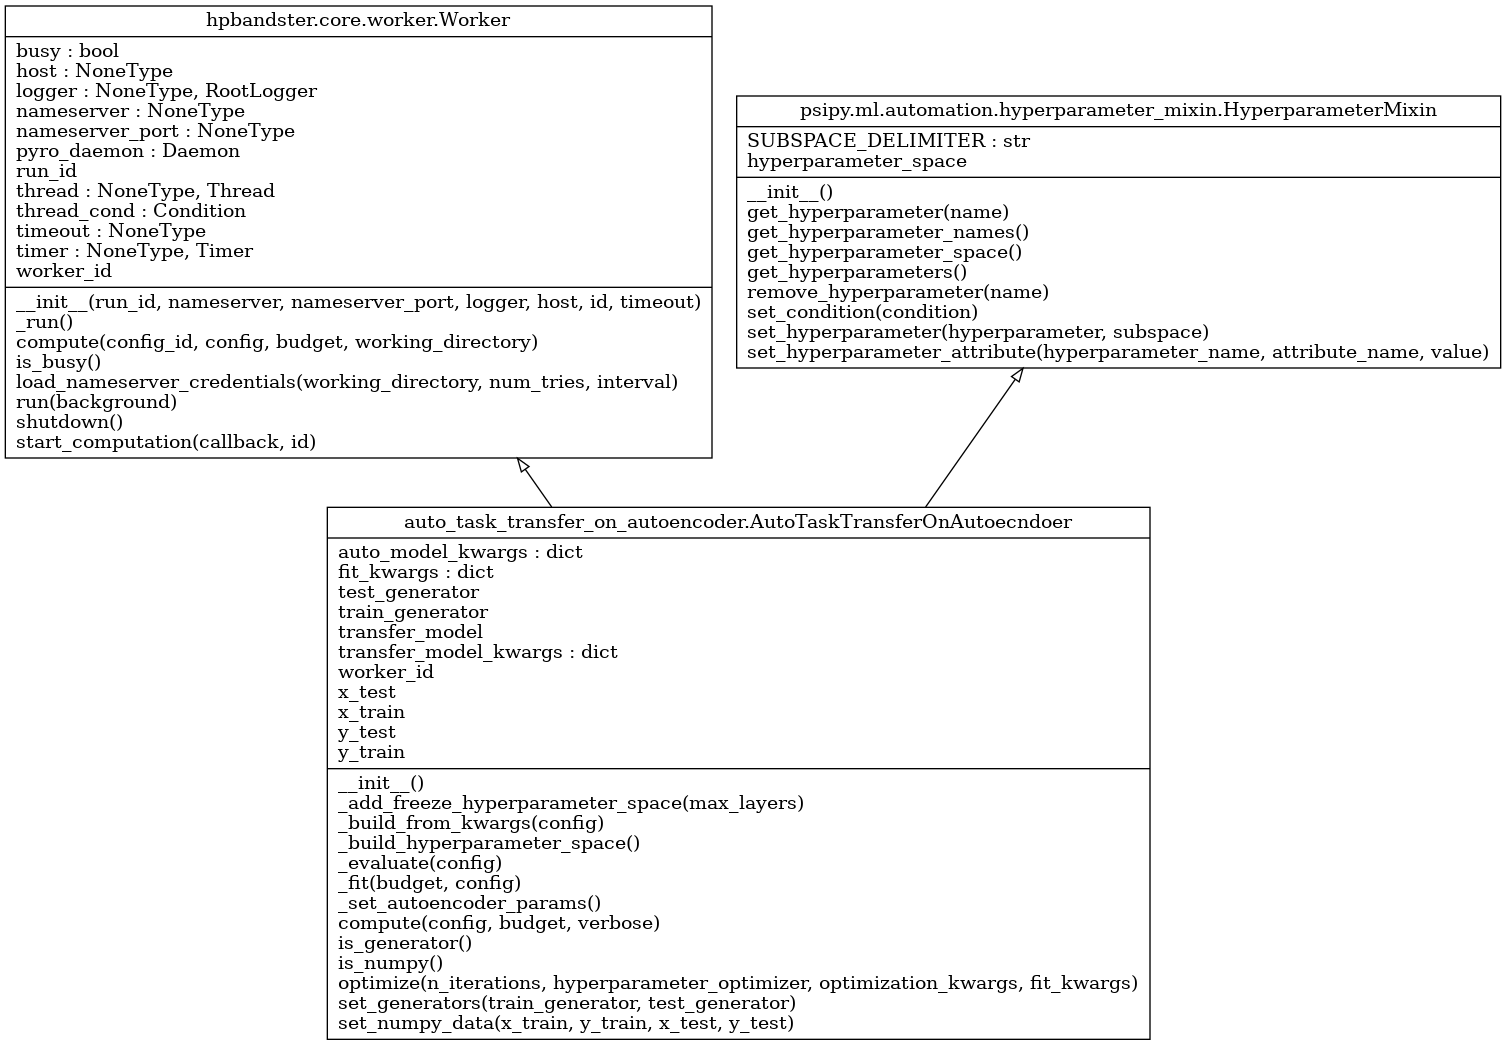
\includegraphics[width=1\textwidth, center]{bilder/Klassendiagramme/AutoTTAE.png}
		\caption[Klassendiagramm AutoTaskTransferOnAutoencoder]{Klassendiagramm AutoTaskTransferOnAutoencoder}
		\label{img:KlassendiagrammAutoTaskTransferOnAutoencoder}
	\end{figure}  
	In Listing \ref{lst:BspAutoTransferSecondCriterionAutoenocder} ist eine einfache Implementierung eines AutoTaskTransferOnAutoencoder dargestellt. Der Konstruktor unterscheidet sich nur an einer Stelle zum Konstruktor des TaskTransferOnAutoencoder. Es wird keine Instanz des SCAE übergeben, sondern ein Pfad zu einem abgespeicherten Modell eines SCAE. 
	Im Gegensatz zur bisherigen Vorgehensweise werden die Trainings und Testdaten mit der Methode $set_generators(..)$  oder $set_numpy_data(..)$ übergeben. Ziel ist es dabei die Komplexität der Methode $optimize(..)$ zu reduzieren. Durch den Aufruf von $optimize(..)$, wird der Optimierungsvorgang gestartet. Die Parameter sind dabei die Anzahl an Iterationen, die Optimierungsstrategie und ein Wörterbuch, welches zusätzliche Einstellungen für die einzelnen Optimierer enthalten kann. In jeder Iteration der Optimierung wird ein neuer TaskTransferOnAutoencoder erstellt und mittels der ausgewählten Hyperparameter und übergebenen Daten trainiert. 
	\begin{lstlisting}[language=python,caption=Beispiel AutoTransferSecondCriterionAutoenocder in Python, label=lst:BspAutoTransferSecondCriterionAutoenocder]
	tscm = AutoTransferConvolutionalSecondCriterionAutoencoder(max_deep_freeze=2,
	path_to_model = path_to_base_model,            
	second_criterion_topology=second_criterion_topology,
	second_criterion_loss = 'categorical_crossentropy',                                                                                                   
	second_criterion_hidden_layer_kwargs = {'activation': 'relu'},
	second_criterion_output_layer_kwargs = {'activation': 'softmax'},
	second_criterion_metrics = {'second_criterion':'accuracy'}
	)
	
	tscm.set_generators(train_datagenerator,test_datagenerator)
	
	
	best_config, history = tscm.optimize(3
	,'RandomSearch'
	,optimization_kwargs = optimization_kwargs)
	\end{lstlisting}
	Das Werkzeug unterstützt derzeit die Optimierer, Zufallssuche, Hyperband und BOHB. Der vom Framework bereitgestellte Parameter Budget wird zur Festlegung der Epochen eingesetzt. Um ein Overfitting zu verhindern, wird ein EarlyStopping Kriterium eingesetzt. 
	Besondere Beachtung muss die Evaluationsmetrik zur Bewertung eines Optimierungslaufes finden. Da ein zu optimierender Hyperparameter die Gewichtung der Verlustfunktion ist, muss dies bei dem Einsatz der Evaluationsmetrik berücksichtigt werden. Die Evaluatiosmetrik kann bei dem Erstellen der Klasse frei gewählt werden.
	
	\subsection{Ergebnis}
	\todo{Auto Ergebnisse}
	Die Gewichtung der beiden Teile der Verlustfunktion hat einen starken Einfluss auf die Modellqualität. In Abbildung x,y,z  ist zu sehen, dass bei einer Gewichtung von abc das Beste Ergebnis erreicht wird. Besonders interessant ist, dass es  (Kurve erläutern.)
	
	
	\section{Datenmenge und 'Greifer beladen'-Klassifikation}
		\todo{Datenmenge Ergebnisse}
		In den vorangegangen Experimenten wurde gezeigt, dass ein Transfer möglich ist und gute Ergebnisse erzielt. In diesem Experiment soll herausgefunden werden, in welchem Maße der Transfer eine Steigerung der Leistung erbringt. Hierzu werden die genutzten Datenmengen auf 200, 2000 und 9749 annotierte Bilder begrenzt.
		
		In Abbildung  sind die Ergebnisse mit verschiedenen Datenmengen dargestellt. Es sticht hervor... 
		
			
		
		
		
		
		
		
		
		
		
		
		
		
		
		
		
		
		
			
		
		
		
		
		
		
		
	
	 % Externe Datei einbinden
\chapter{Fazit}
\label{chap:Fazit}
Die Arbeit schließt mit einer Zusammenfassung der Inhalte ab, auf welche eine kritische Auseinandersetzung mit verschiedenen Ergebnissen der Abschlussarbeit folgt und durch einen ausführlichen Blick auf mögliche Erweiterungen und weitere geleistete Arbeiten komplettiert wird.
 
	\section{Zusammenfassung}
	\label{sec:Zusammenfassung}
	Zu Beginn der Arbeit wurde die zu bearbeitende Problemstellung erläutert, anschließend wurden die theoretischen Hintergründe, das Umfeld der Problemstellung und die Datensätze vorgestellt. Der Hauptteil der Arbeit beschäftigt sich mit aufeinander aufbauenden Ansätzen des Transferlernens. Im ersten Schritt wurde gezeigt, dass ein Ansatz, ausgehend von einer nicht fokussierten Repräsentation fehlschlägt. Darauf folgend wurde ein Multi-Task-Ansatz zum gleichzeitigen Fokussieren und Lösen einer Regressionsaufgabe vorgestellt und evaluiert. Insbesondere die gefundene Repräsentation hat dabei deutlich die aktuelle Domäne widergespiegelt. Darauf aufbauend wurde ein Ansatz des modellbasierten Transferlernen vorgestellt. Die Ergebnisse erreichen eine ähnliche Leistung wie ein Modell, welches von einem Experten erstellt wurde. Zur \ac{hpo} der Aufgaben-Gewichtungsparameter wurde eine \ac{automl}-Erweiterung eingesetzt. Dabei hat sich gezeigt, dass der Hyperparameter einen deutlichen Einfluss auf das Ergebnis hat und die automatische Suche hilfreich ist. Abschließend wurde gezeigt, dass die Transfer-Lösung insbesondere für geringe Datenmengen gute Ergebnisse liefern kann. Begleitend zu der Vorstellung der Ansätze wurde jeweils eine Python-Implementierung des Ansatzes vorgestellt. 
	
	\section{Kritische Reflexion}
	\label{sec:KritischeReflexion}
	Eine  Abschlussarbeit wird immer in einem Zeitlich begrenzenden Rahmen durchgeführt. Diese zeitliche Begrenzung führt in manchen Fällen dazu, dass manche Teilaspekten der Arbeit nur angerissen oder mit  begrenzenden Mittel bearbeitet werden können. In dieser Arbeit betrifft dies insbesondere das Thema \ac{automl}, konkret den Versuch \ref{subsec:AutoMLExperiment}. Das zugehörige Python-Module \ac{autottae} baut auf den anderen beiden Modulen auf und wurde somit recht spät in der Masterarbeit bearbeitet. Eine Optimierungs-Iteration dauert circa einen Tag. Diese beiden Faktoren haben dazu geführt, dass der Versuch nur mit 3 Iterationen durchgeführt wurde. Hier empfiehlt es sich eine Optimierung mit deutlich mehr Iterationen durchzuführen.
	
	Auf Grund der Einfachheit (vier Ausgangsneuronen) wurde für  Aufgabe 'Rahmen um Greifer' eine Regression eingesetzt. In der Regel werden für Objekterkennungsaufgaben andere Techniken wie z.B. der bereits erwähnte \ac{ssd}-Ansatz eingesetzt. Durch eine explizite Lokalisierung und Klassifizierung werden oft bessere Ergebnisse erzielt.
	
	Die bisherigen Versuche wurden alle in der selben Domäne, mit  Bilder und dem Greifer durchgeführt. Die gewählten Ansätze wurden für diese Umgebung gewählt. Die Aussagekraft auf andere Domänen oder Umgebungen mit weniger stark ausgeprägten Merkmalen wie ein Greifer ist schwach und sollte in weiteren Versuchen untersucht werden.    
							
	\section{Ausblick und weitere Arbeiten}
	\label{sec:AusblickWeitereArbeiten}
	In diesem letzten Unterkapitel werden weitere (vorläufige) Ergebnisse dargestellt und ein Blick auf mögliche Erweiterungen geworfen.

	\subsection{Transfer auf Greiferdatensatz}
	\label{subsec:TransferGreiferDatensatz}
 	Die Annotationskosten sind je nach Art von Annotation und Aufwand unterschiedlich. Eine einfache Zuordnung eines Bildes zu einer, von zwei Klassen liegt dabei im einstelligen Cent-Bereich. Die Markierung eines Objektes in einem Bild mittels Rahmen verursacht Kosten im zweistelligen Cent-Bereich und die Markierung von Winkeln in einem Bild kann mehr als einen Euro kosten. In Experiment \ref{sec:TransferDatenmenge} und \ref{subsec:TransferLogs} wurde gezeigt, dass der Transfer für die Aufgabe 'Greifer beladen?' funktioniert und insbesondere bei wenigen Daten stark ist. Falls es möglich ist, dass ein Transfer von der Aufgabe 'Greifer beladen?' zu der Aufgabe 'Rahmen um Greifer' möglich ist, kann sehr viel Geld gespart werden, da die Annotationen deutlich teurer sind. 
 	
 	Im ersten Versuch ist der Transfer auf dem Greiferdatensatz fehlgeschlagen, durch weitere Arbeiten an dem Problem konnte eine Verbesserung erzielt werden. Zu den weiteren Arbeiten zählen, das Entfernen von Bildern bei denen der Greifer über den Rand des Bildes hinausgeht. Diese Bildern können durch eine Modifikation der Kameraposition am Kran nicht mehr vorkommen. Weitere Verbesserungen konnten durch Regularsierungstechniken erzielt werden. Im Anhang \ref{appendix:TTAEGreifer } ist die aktuelle Modellzusammenfassung zu finden.
 	In Abbildung \ref{img:TTGrappleIoU} sind die Ergebnisse der Aufgabe 'Rahmen um Greifer' dargestellt. Bei einem Schwellenwert von 0.5 wird eine Leistung von 96\% Erreicht, bei einem Schwellenwert 0.8 eine Leistung von 55\%. Bei genauerer Betrachtung der Vorhersagen fällt auf, dass der Greifer gefunden wird. Die genaue Form des Greifers wird nicht immer korrekt Vorhergesagt. Dieses Verhalten ist auch in Abbildung \ref{img:TTGrappleLabelVsPred} zu sehen. In dieser Art von Abbildungen werden die vorhersagen gegen die Beschriftungen aufgetragen. Bei einer perfekten Vorhersage befinden sich alle Datenpunkte auf der Diagonale. Sowohl in der Darstellung der Rahmenhöhe, als auch der Rahmenbreite, ist zu sehen, dass die Vorhersage zur Beschriftung passt, aber sich noch verbessern kann. In Abbildung \ref{img:TTGrappleEinbettungVorhersage} sind die für den Schwellenwert 0.8 falsch vorhergesagten Datenpunkte in der Einbettung lila eingefärbt. Die falschen Vorhersagen verteilen sich über alle Datenpunkte. Mit Blick auf die Einfärbung der x und y Position des Greifers \ref{img:TTGrappleEmb} zeigt sich in den Einbettungen die Position des Greifers im Bild. Widerspiegelnd zu den Vorhersageergebnissen ist in der Einbettung die genaue Ausprägung des Greifers schwach repräsentiert.
 	
 	 
 	\begin{figure}[h]
 		\centering
 		\begin{subfigure}[c]{0.32\textwidth}			
 			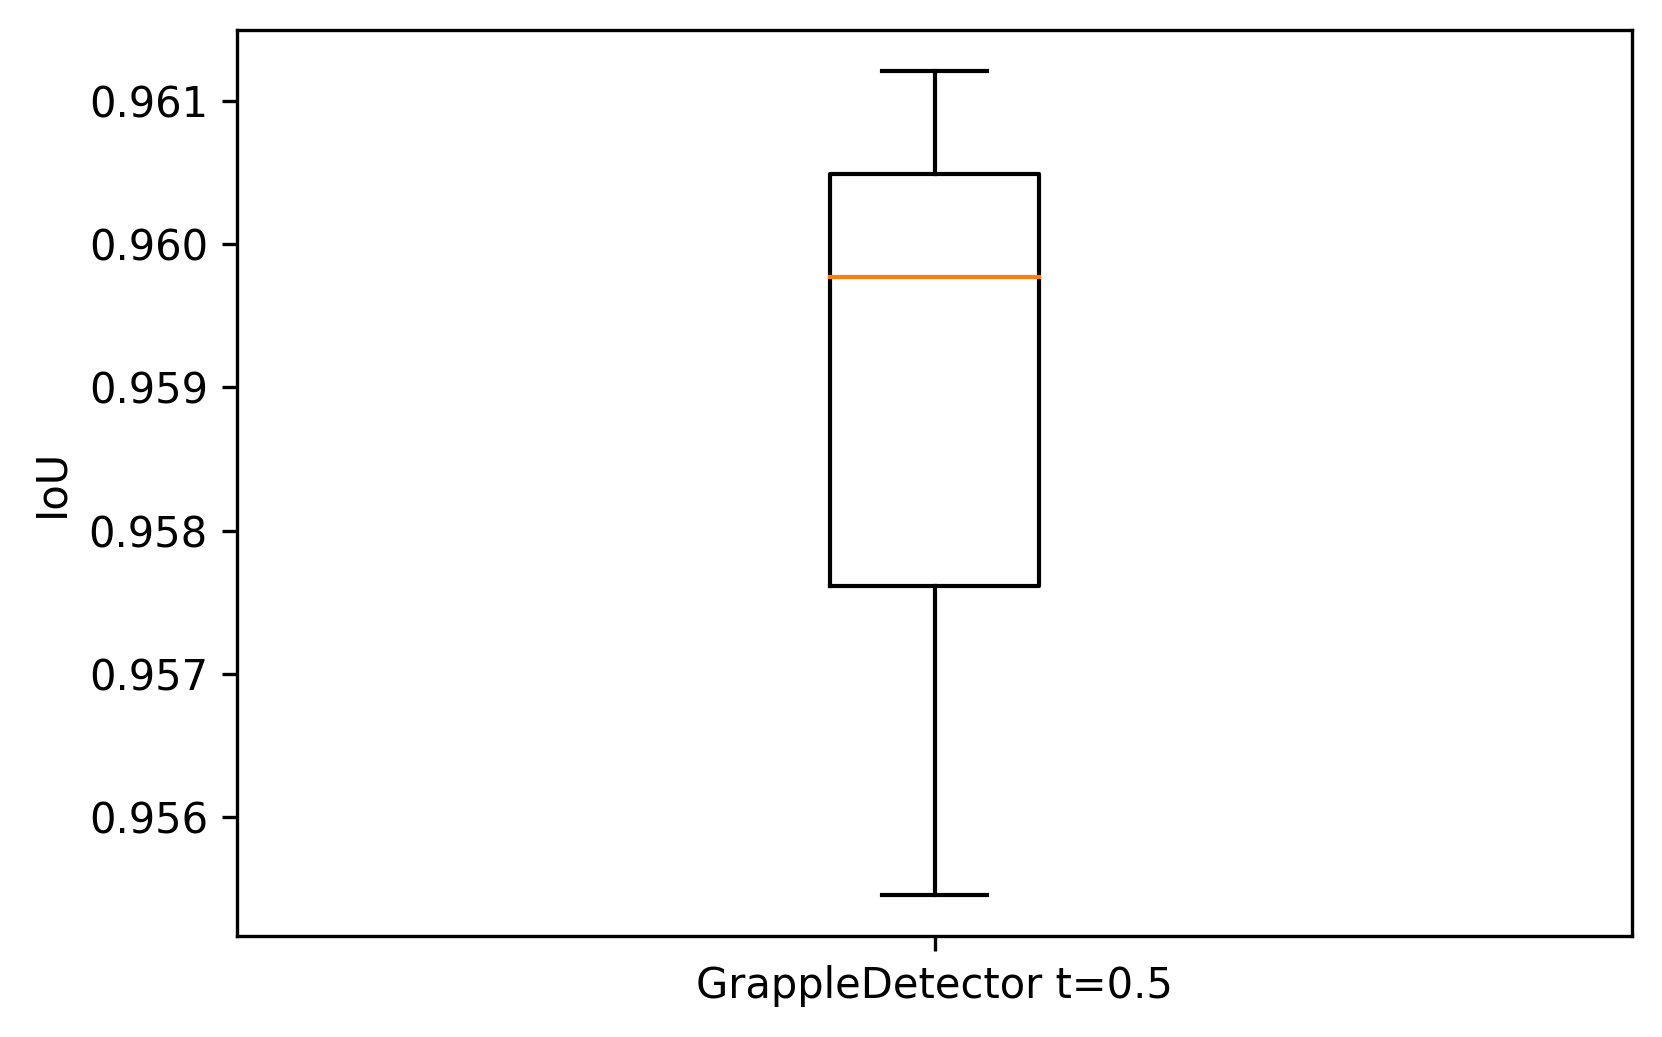
\includegraphics[width=1\textwidth]{bilder/FazitUndAusblick/Grapple_TTAE_Res/IoU_TTAE_05.png}
 			\subcaption{Schwellenwert 0.5}			
 		\end{subfigure}
 		\begin{subfigure}[c]{0.32\textwidth}			
 			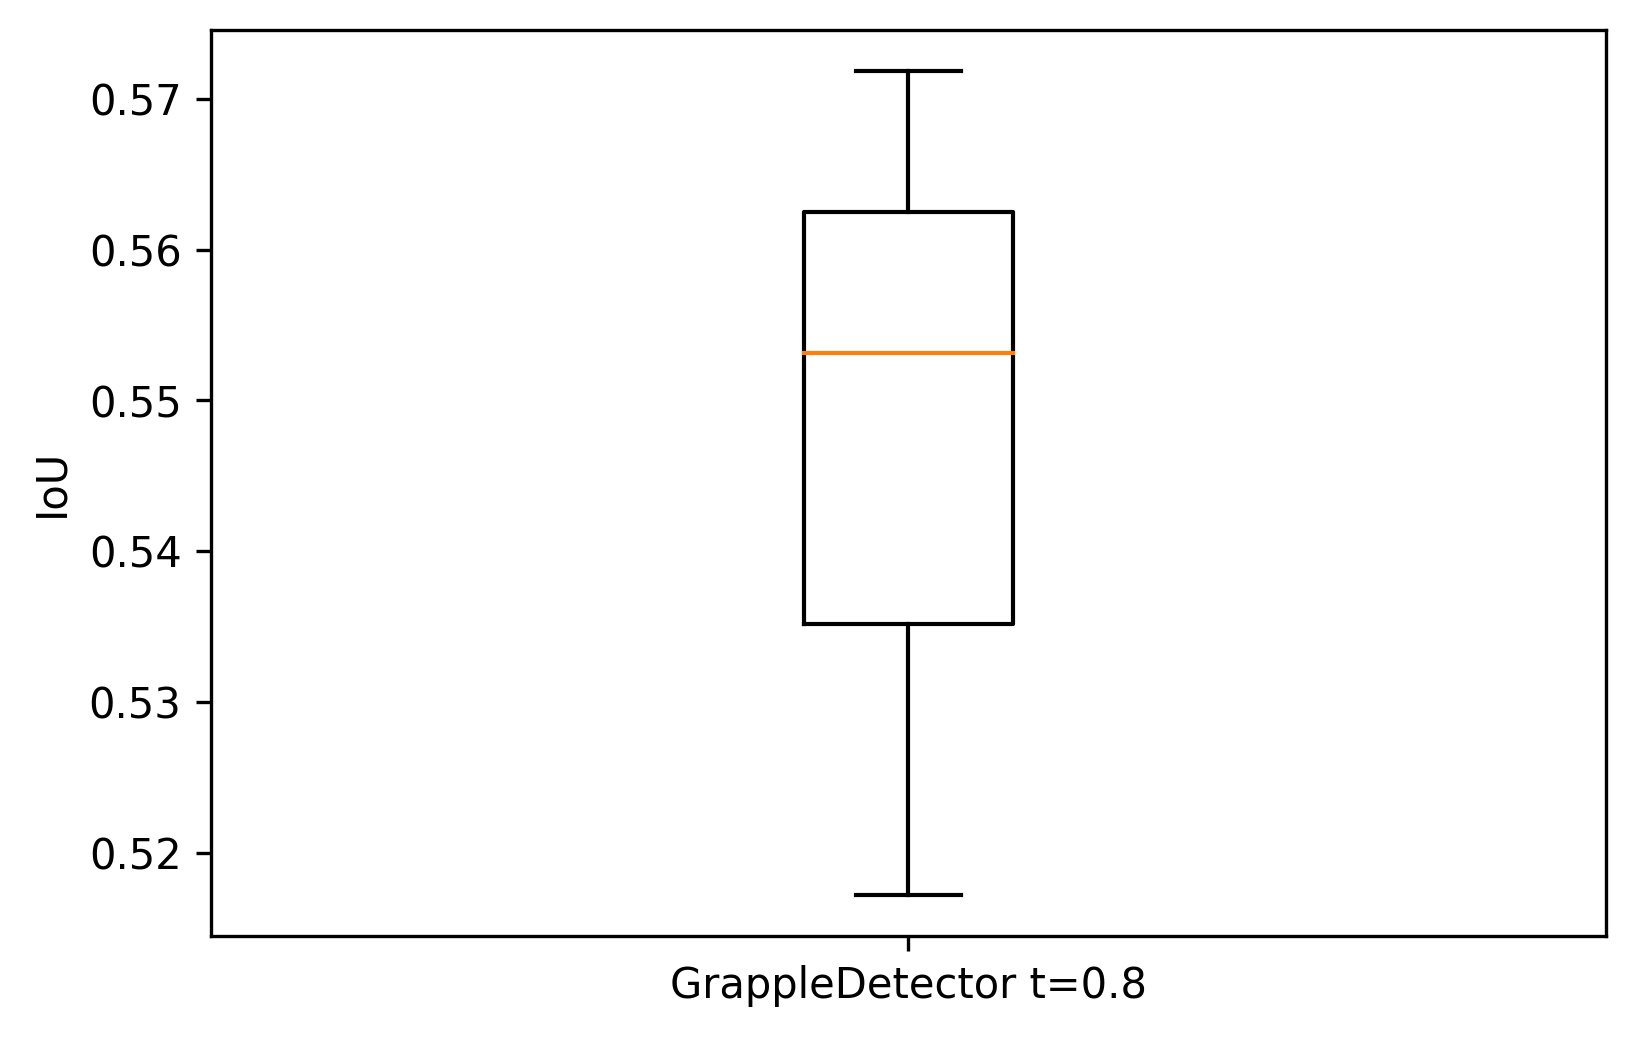
\includegraphics[width=1\textwidth]{bilder/FazitUndAusblick/Grapple_TTAE_Res/IoU_TTAE_08.png}
 			\subcaption{Schwellenwert 0.8}			
 		\end{subfigure}
 		\begin{subfigure}[c]{0.32\textwidth}			
 			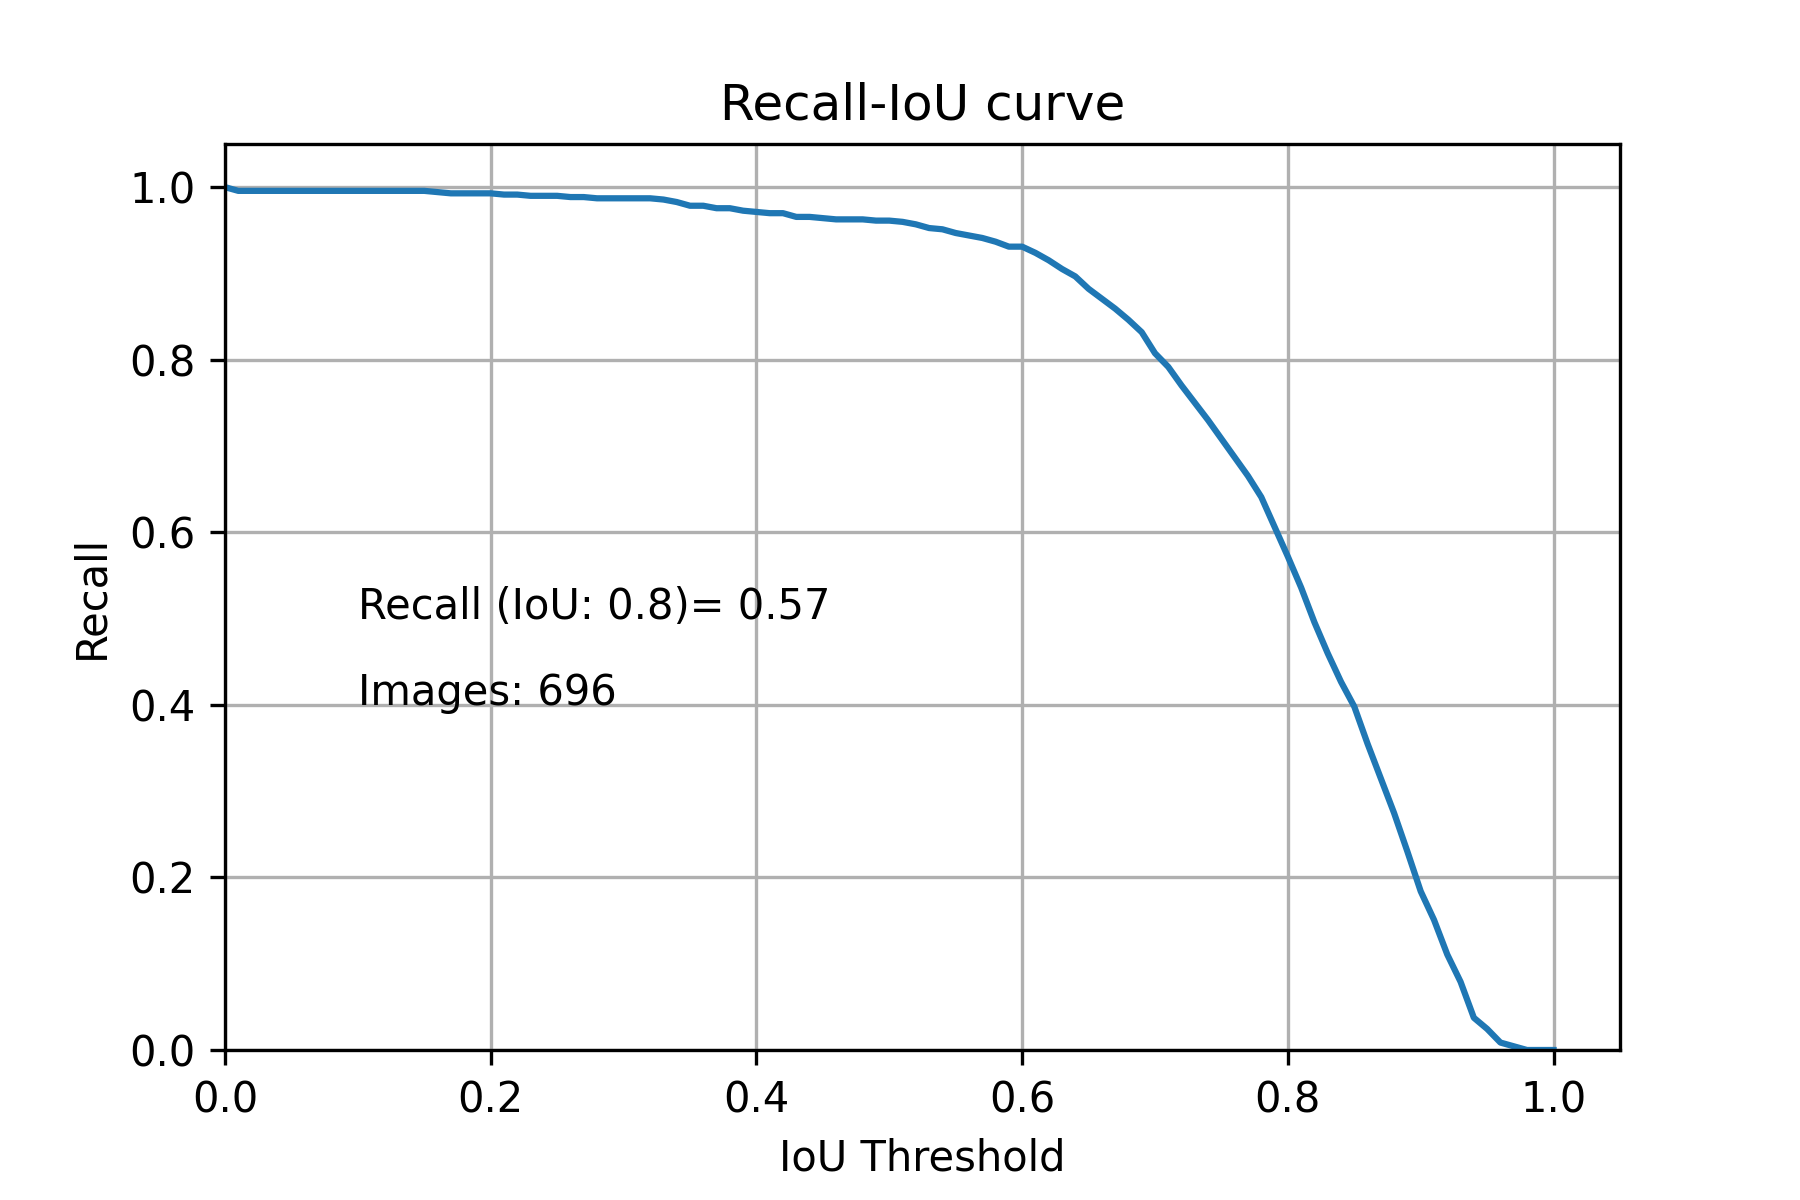
\includegraphics[width=1\textwidth]{bilder/FazitUndAusblick/Grapple_TTAE_Res/Recall_IoU_TTAE.png}
 			\subcaption{IoU-Recall-Curve}			
 		\end{subfigure}
 		\caption{IoU TTAE Greifer}
 		\label{img:TTGrappleIoU}
 	\end{figure}
 
 	 	\begin{figure}[h]
 		\centering
 		\begin{subfigure}[c]{0.49\textwidth}			
 			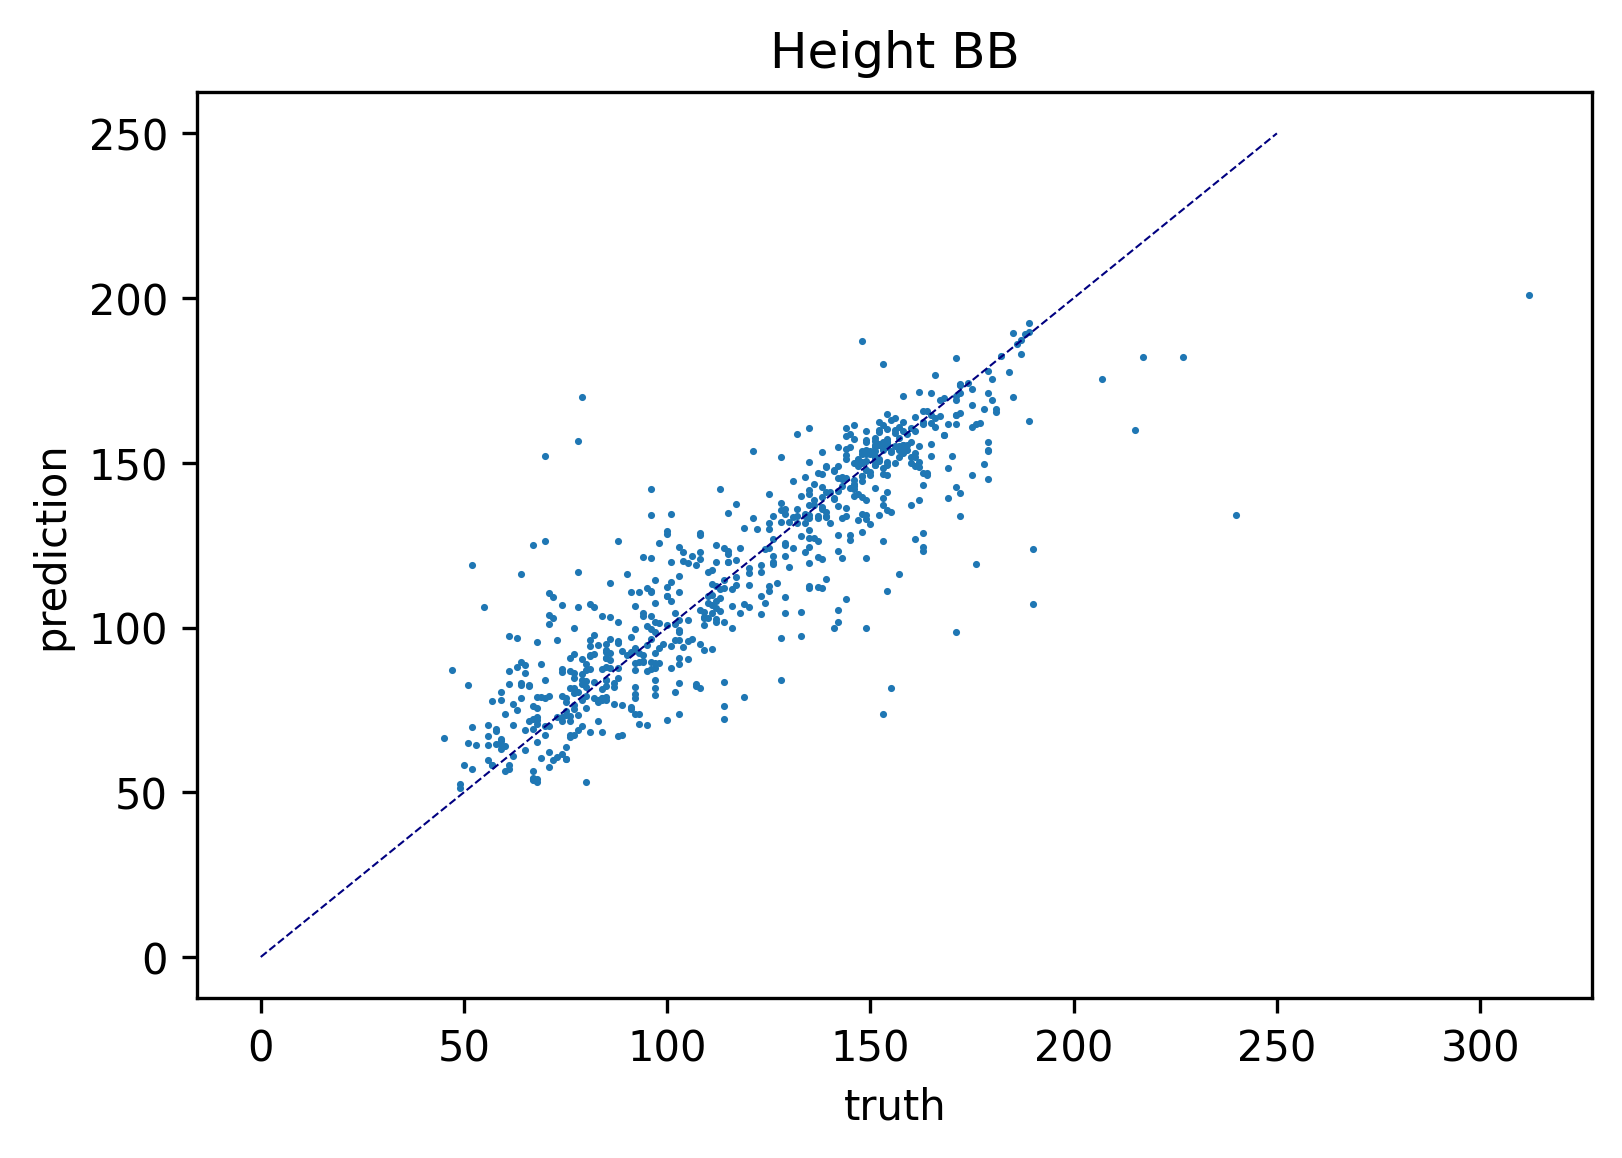
\includegraphics[width=1\textwidth]{bilder/FazitUndAusblick/Grapple_TTAE_Res/Height_BB.png}
 			\subcaption{Rahmenhöhe}			
 		\end{subfigure}
 		\begin{subfigure}[c]{0.49\textwidth}			
 			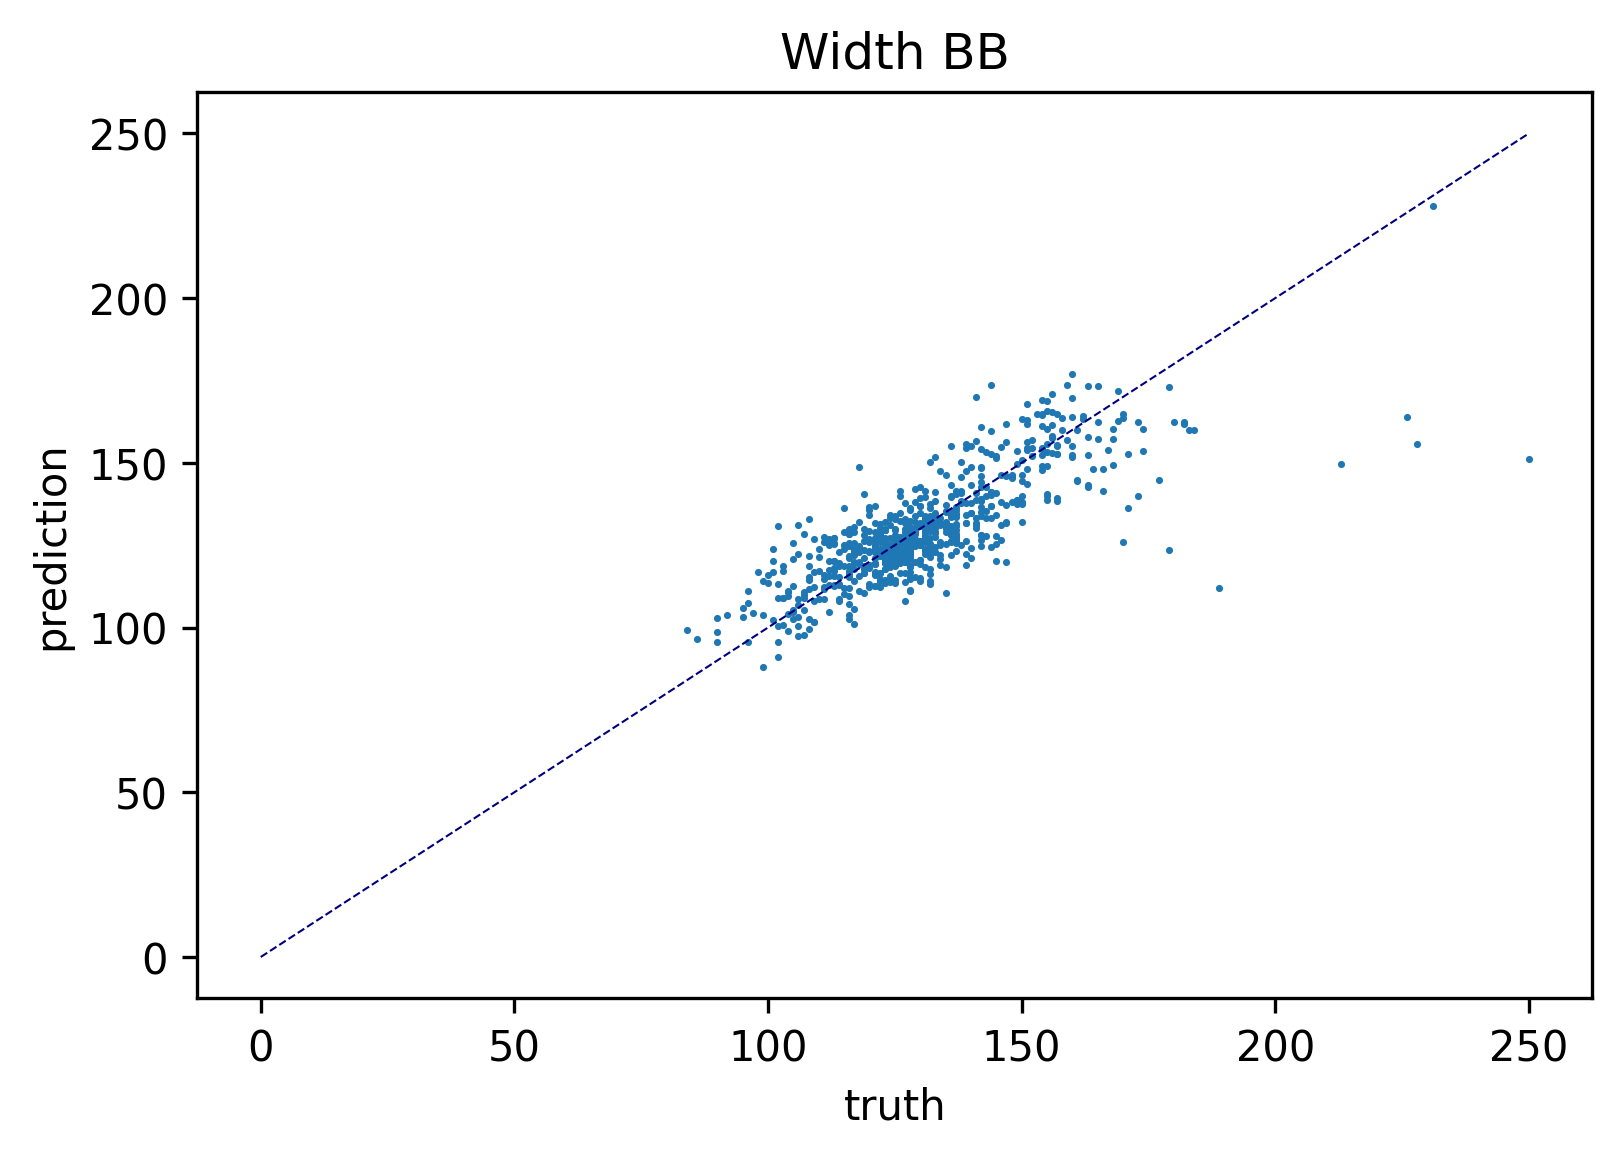
\includegraphics[width=1\textwidth]{bilder/FazitUndAusblick/Grapple_TTAE_Res/Width_BB.png}
 			\subcaption{Rahmenbreite}			
 		\end{subfigure}  
 		\caption{Beschriftung vs Vorhersage}
 		\label{img:TTGrappleLabelVsPred}
 	\end{figure}
 
 	\begin{figure}[h]
 		\centering
 		\begin{subfigure}[c]{0.45\textwidth}			
 			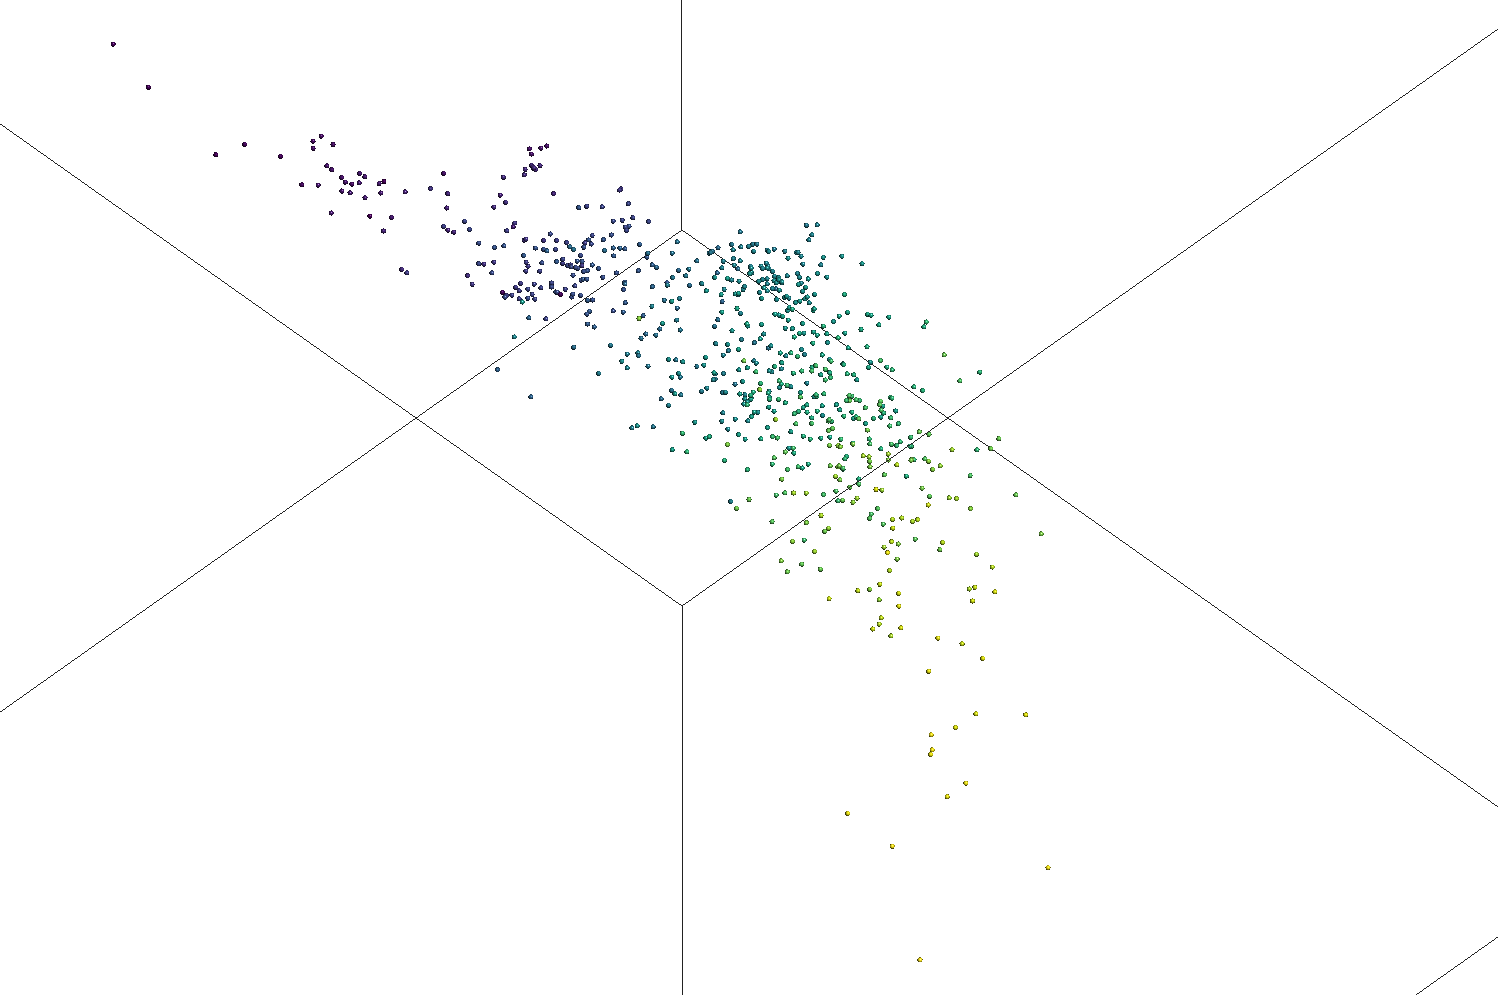
\includegraphics[width=1\textwidth]{bilder/FazitUndAusblick/Grapple_TTAE_Res/TT_Emb_y.png}
 			\subcaption{Einbettung y-Position Greifer}			
 		\end{subfigure}
 		\begin{subfigure}[c]{0.45\textwidth}			
 			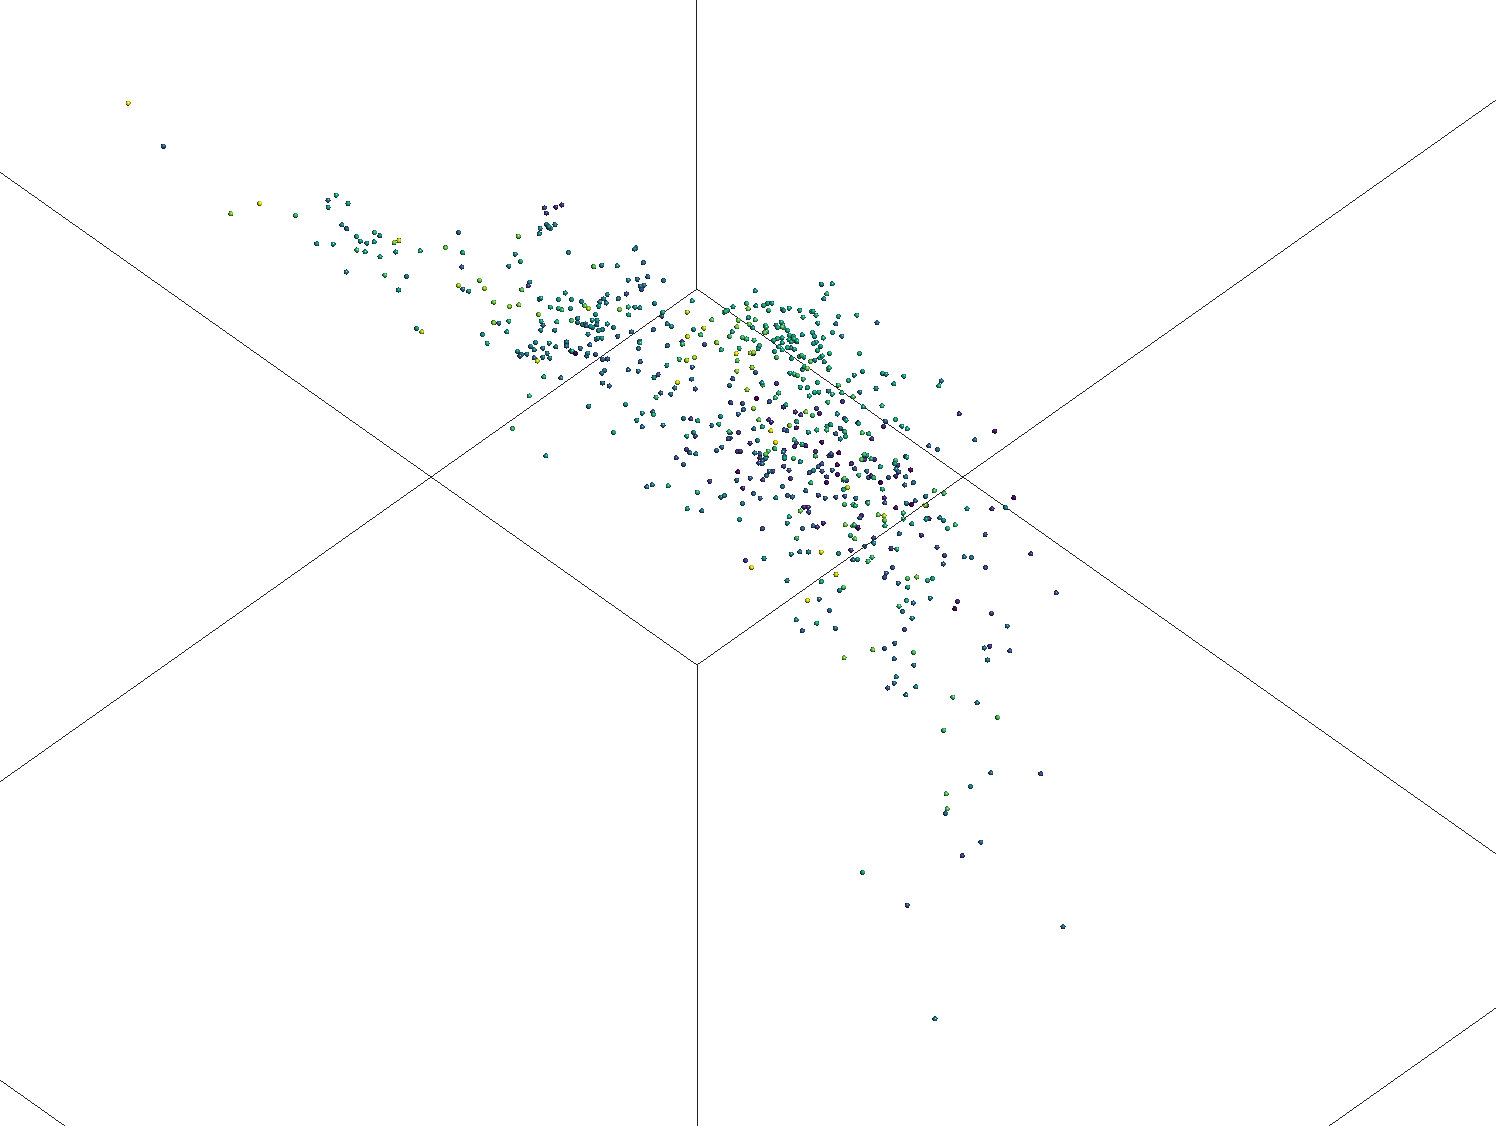
\includegraphics[width=1\textwidth]{bilder/FazitUndAusblick/Grapple_TTAE_Res/TT_Emb_x.png}
 			\subcaption{Einbettung x-Position Greifer}			
 		\end{subfigure}
 		\begin{subfigure}[c]{0.6\textwidth}			
 			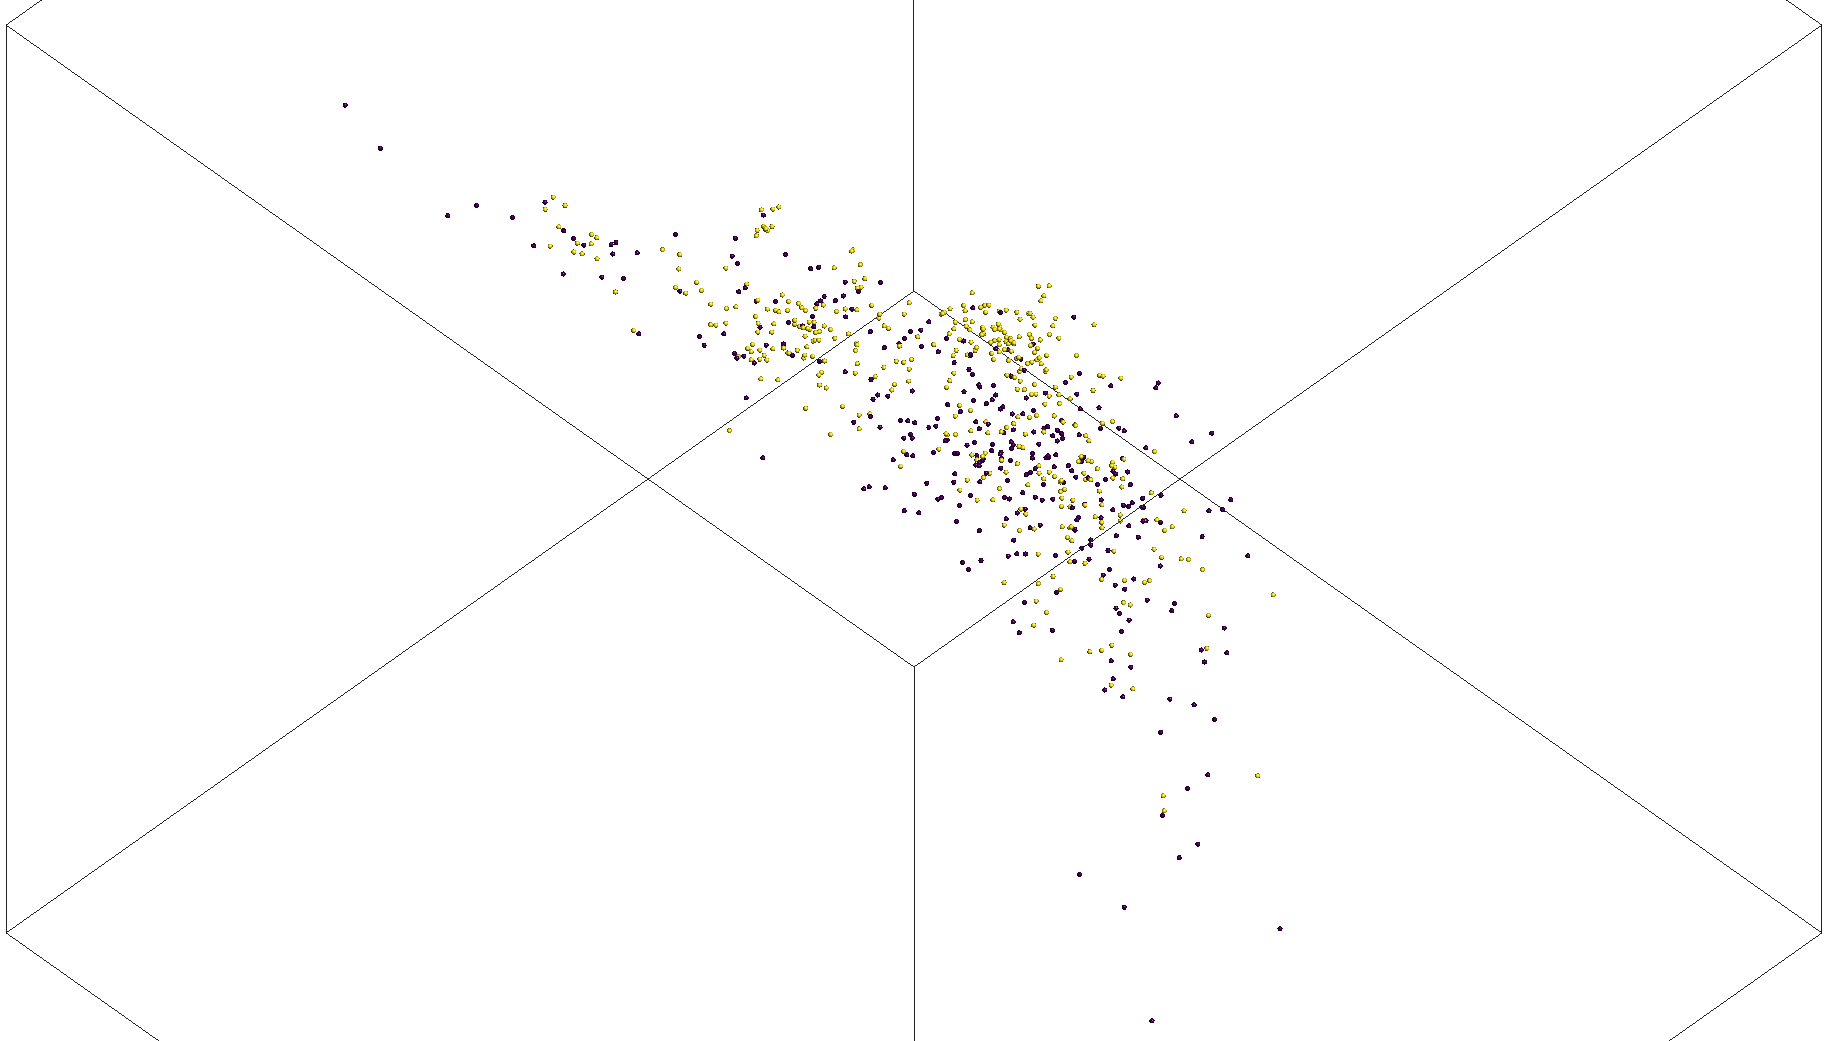
\includegraphics[width=1\textwidth]{bilder/FazitUndAusblick/Grapple_TTAE_Res/TT_Emb_pred.png}
 			\subcaption{Einbettung mit Vorhersage}		
 			\label{img:TTGrappleEinbettungVorhersage}	
 		\end{subfigure}
 		\caption{Einbettung TTAE Greifer}
 		\label{img:TTGrappleEmb}
 	\end{figure}
 	
	\subsection{Autocrane-Datensatz}
	\label{subsec:AutocraneDatensatz}	
	Im Rahmen der Arbeit wurde ein Datensatz erarbeitet und Projektpartnern zur Verfügung gestellt. Eine spätere Veröffentlichung des Datensatzes unter der Adresse psiori.com ist geplant. Der Datensatz soll zu allgemeinen akademischen und pädagogische Zwecken genutzt werden dürfen. Alternativ kann Zugang zu dem Datensatz über die E-Mail-Adresse info@psiori.com angefragt werden.

	\subsection{Erweiterung: Multi-Task-Learning-Ansatz}
	\label{subsec:MehrfacheAufgaben}
	Multi-Task-Learning beschränkt sich nicht auf zwei Aufgaben. Die gezeigte Lösung kann um weitere Aufgaben erweitert werden. In Abbildung \ref{img:AusblickMultiTaskAnsatz} ist der erweitere Ansatz schematisch abgebildet. Wie in den bisherigen Ansätzen werden ausgehend von der Code-Schicht weitere Aufgaben bearbeitet. Durch die weiteren Aufgaben wird die Gewichtung der einzelnen Aufgaben noch schwerer. In Experiment \ref{subsec:AutoMLExperiment}  wurde gezeigt, dass AutoML bei der Gewichtung helfen kann. Dieser erweiterte Ansatz soll in einem Anschlussprojekt für die Praxistauglichkeit untersucht werden. Der Aufwand, das bisher entwickelte Python-Modul zu erweitern, wird sich dabei in Grenzen halten. Insbesondere müssen im Konstruktor Erweiterungen zum Erstellen der Modelle der weiteren Aufgaben getätigt werden. An anderen Stellen wie z. B. der Methode zum Trainieren des Gesamtmodells wird keine Erweiterung notwendig sein, da bereits mit Listen gearbeitet wird.
	\begin{figure}[h]
		\centering
		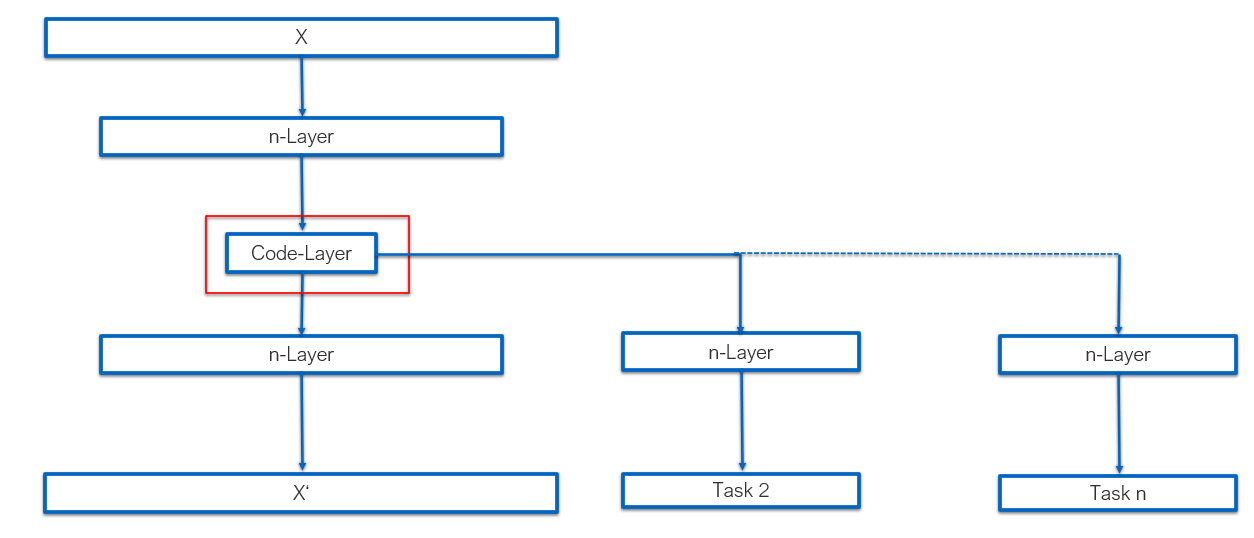
\includegraphics[width=0.6\textwidth, center]{bilder/FazitUndAusblick/MultiTaskAnsatz.PNG}
		\caption{Multi-Task-Learning-Ansatz}
		\label{img:AusblickMultiTaskAnsatz}
	\end{figure}

	\subsection{Flexibilität der Werkzeuge}
	\label{subsec:FlexibilitätDerWerkzeuge}
	Die bisherigen Module sind starr bei der Anwendung. Es ist notwendig, ein Multi-Task-Learning-Modell zu erstellen, um anschließend den modellbasierten Transfer durchzuführen. Soll ein neuer modellbasierter Transfer durchgeführt werden, ist es zwingend erforderlich dies ausgehend des Multi-Task-Learning-Modells durchzuführen. Es ist nicht möglich einen modellbasierten Transfer, ausgehend von einem vorherigen Transfer durchzuführen. 
	Als mögliche Erweiterung der Module ist es empfehlenswert, eine Flexibilisierung des Gesamtansatzes durchzuführen. Durch eine Anpassung bei der Modellerstellung der Module, ist es möglich, dass die Abfolge nicht mehr notwendig ist. Es ist vorstellbar, dass ein neues Modell ausgehend von einer Architekturdefinition komplett neu trainiert wird, oder ausgehend von einem Autoencoder-Modell mit null bis beliebig vielen weiteren Aufgaben trainiert werden kann. Konkret muss im Konstruktor der Module eine Zusammenführung der bisher getrennten Ansätze durchgeführt werden.     


	    % Externe Datei einbinden
% ------------------------------------------------------------------

\label{lastpage}

% Neue Seite
\cleardoublepage

% Backmatter mit normalem Zeilenabstand setzen
\singlespacing

% Römische Ziffern für die "Back-Matter", fortlaufend mit "Front-Matter"
\pagenumbering{roman}
%\setcounter{page}{\value{frontmatterpage}}
\setcounter{page}{0}
% Abkürzungsverzeichnis
\addchap{\hsmaabbreviations}
\begin{acronym}[IEEE]
	\acro{ml}[ML]{maschinellen Lernens}
	\acro{automl}[AutoML]{automatisierte maschinelle Lernen}
	
	\acro{tfae}[TFAE]{TaskFocusingOnAutoencoder}
	\acro{ttae}[TTAE]{TaskTransferOnAutoencoder}
	\acro{autottae}[AutoTTAE]{AutoTaskTransferOnAutoencoder}
	
	\acro{nas}[NAS]{Neural Architecture Search}
	\acro{hpo}[HPO]{Hyperparameter-Optimierung}	
	\acro{cae}[CAE]{Convolutional Autoencoder}	
	
	\acro{ssd}[SSD]{Single Shot MultiBox Detector}
	
	\acro{mtl}[MTL]{Multi-Task-Lernen}		
	\acro{miso}[MISO]{Multi-Input Single-Output}	
	\acro{simo}[SIMO]{Single-Input Multi-Output}	
	\acro{mimo}[MIMO]{Multi-Input Multi-Output}	
	

	\acro{sh}[SH]{Successive Halving}	
	
	\acro{iou}[IoU]{Intersection over Union}	
\end{acronym}


% Tabellenverzeichnis erzeugen
\cleardoublepage
\phantomsection
\addcontentsline{toc}{chapter}{\hsmalistoftables}
\listoftables

% Abbildungsverzeichnis erzeugen
\cleardoublepage
\phantomsection
\addcontentsline{toc}{chapter}{\hsmalistoffigures}
\listoffigures

% Listingverzeichnis erzeugen
\cleardoublepage
\phantomsection
\addcontentsline{toc}{chapter}{\hsmalistings}
\lstlistoflistings

% Literaturverzeichnis erzeugen
\begin{flushleft}
\printbibliography
\end{flushleft}

% Index ausgeben. Wenn Sie keinen Index haben, entfernen Sie einfach
% diesen Teil.
%\cleardoublepage
%\phantomsection
%\addcontentsline{toc}{chapter}{\hsmaindex}
%\printindex

% Anhang. Wenn Sie keinen Anhang haben, entfernen Sie einfach
% diesen Teil.
\appendix
\chapter{Anhang Basislinie Greifer}
\label{appendix:BasislinieGreifer}


\begin{figure}[h]
	\centering
	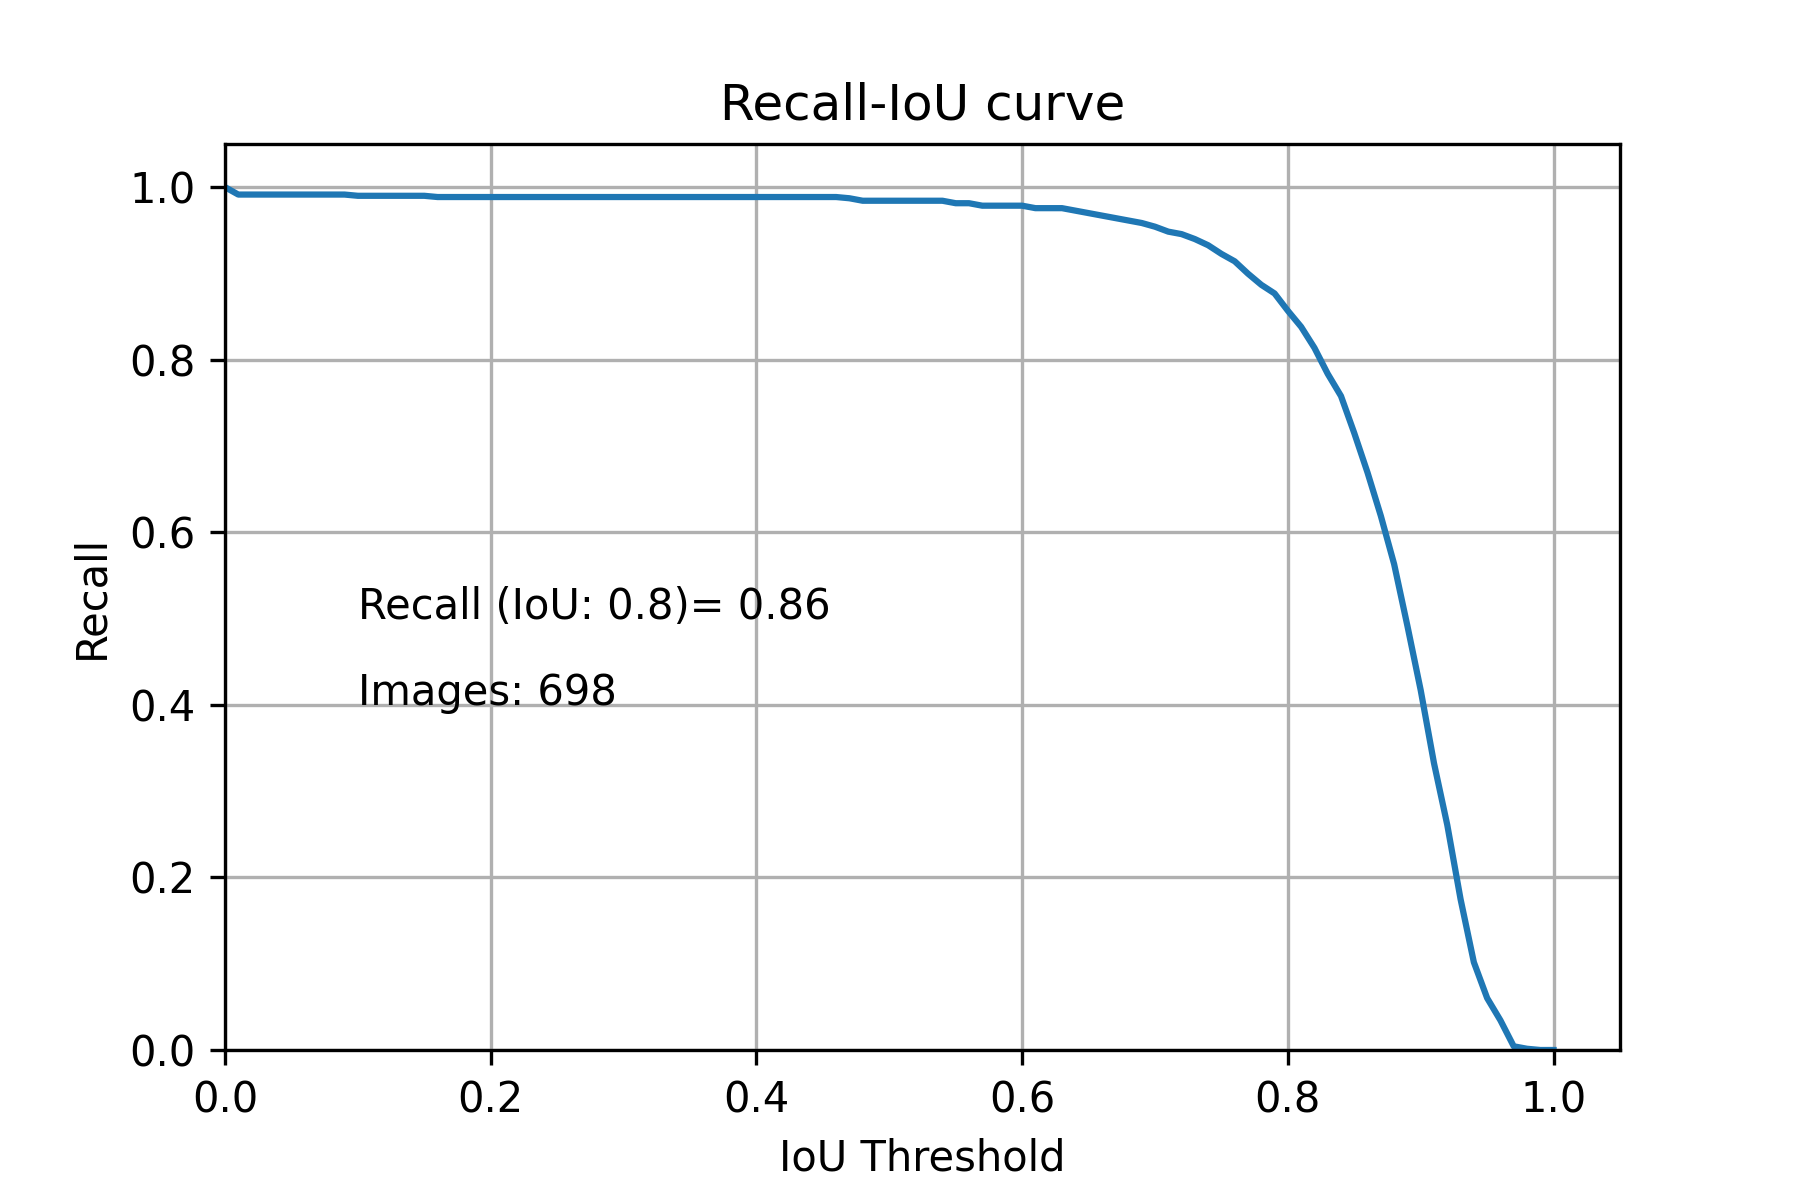
\includegraphics[width=1\textwidth, center]{bilder/Anhang/Baseline/Grapple/RecallIoU_Validation.png}
	\caption[RecallIoUGrappleBaseline]{Basislinie Greifererkennung}
	\label{img:RecallIoUGrappleBaseline}
\end{figure}	

\chapter{Basislinie 'Greifer beladen?'s}
\label{appendix:BasislinieBaumstämme}

\begin{figure}[h]
	\centering
	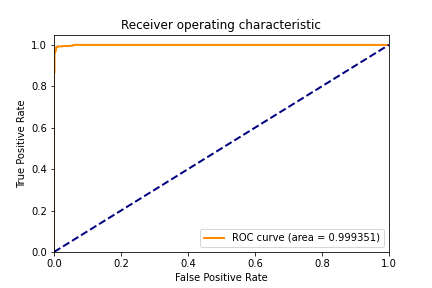
\includegraphics[width=0.5\textwidth, center]{bilder/Anhang/Baseline/Logs/Logs_validation/Logs_Baseline_ROC.png}
	\caption[Baumstammklassifikation Basislinie ROC]{receiver operating characteristic}
	\label{img:BaselineLogsROC}
\end{figure}	

\begin{figure}[h]
	\centering
	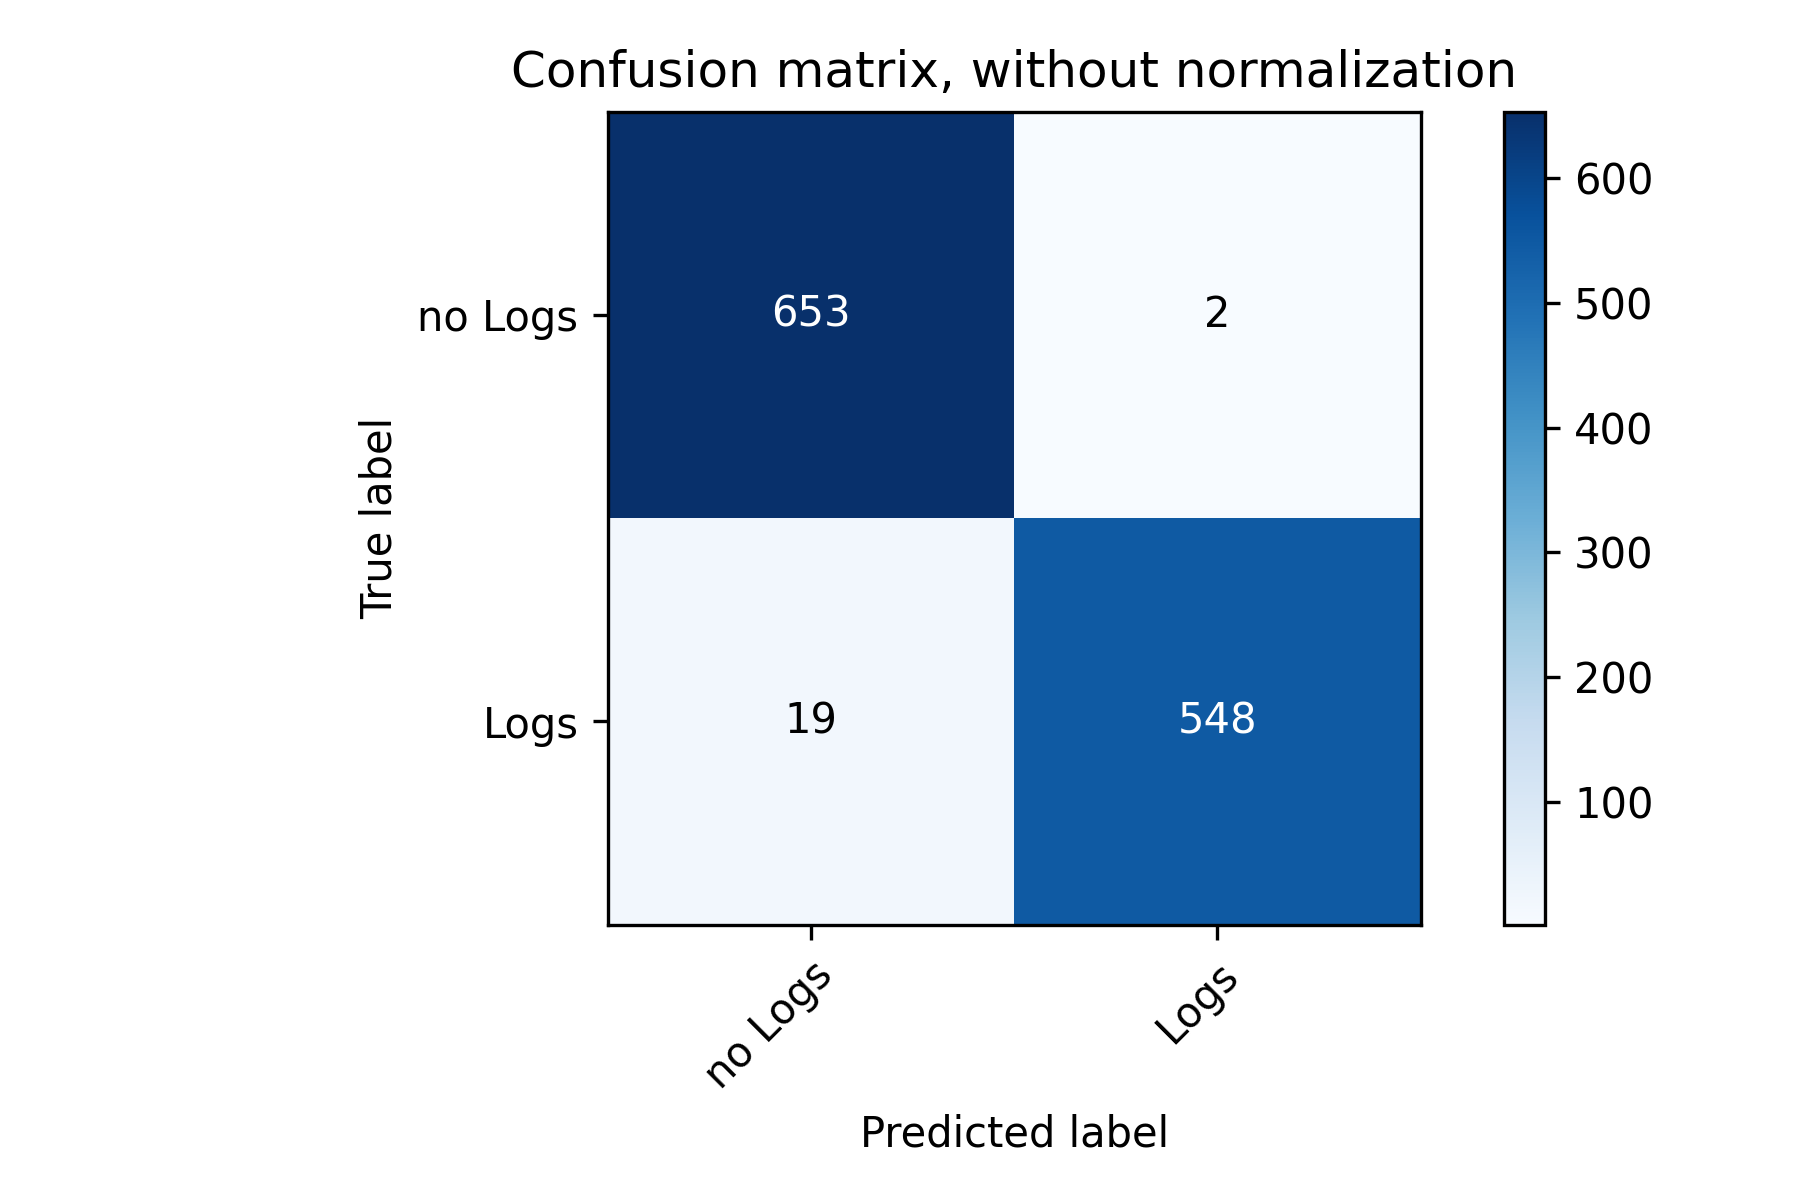
\includegraphics[width=0.6\textwidth, center]{bilder/Anhang/Baseline/Logs/Logs_validation/Logs_Baseline_Confusion_Matrix.png}
	\caption[Konfusionsmatrix Baumstammklassifikation Basislinie]{Konfusionsmatrix}
	\label{img:BaselineLogsConfusionMatrix}
\end{figure}	

\begin{figure}[h]
	\centering
	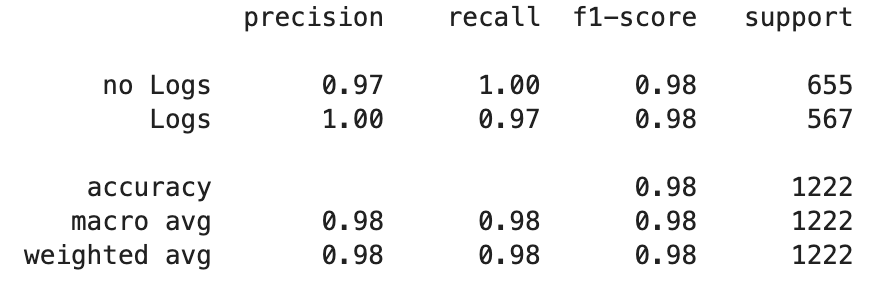
\includegraphics[width=0.6\textwidth, center]{bilder/Anhang/Baseline/Logs/Logs_validation/classification_report.png}
	\caption[Klassifikationsreport Baumstammklassifikation Basislinie]{Klassifikationsreport}
	\label{img:BaselineLogsKlassifikationsreport}
\end{figure}	

\chapter{Anhang  Greifererkennung}
\label{appendix:Greifererkennung}

	\section{Greifererkennung auf Autoencoder}
	\label{appendix:GreifererkennungAufAutoencoder}
	
		\begin{table}[ht]
		\centering
		\begin{tabularx}{\textwidth}{lll}
			\textbf{Versuch}  & \textbf{IoU t=0.5} & \textbf{IoU t=0.8}  	 \\ \hline 
			1 & 0.3565 & 0.0127 \\
			2 & 0.3735 & 0.0227 \\
			3 & 0.3821 & 0.0383 \\ 
		\end{tabularx}
		\caption{Einzelwerte Boxplot IoU Greifererkennung auf Autoencoder}
		\label{table:EinzelwerteBoxplotIoUGreifererkennungaufAutoencoder}
	\end{table}

	\section{Mutli-Task Greifererkennung}
	\label{appendix:MutliTaskGreifererkennung}
	
	\begin{table}[ht]
	\centering
	\begin{tabularx}{\textwidth}{lll}
		 \textbf{Nr.}  & \textbf{IoU t=0.5} & \textbf{IoU t=0.8}  	 \\ \hline 
		1 & 0.8638 & 0.2254 \\
		2 & 0.9899 & 0.7555 \\
		3 & 0.8571  & 0.2131 \\
		4 & 0.9966 & 0.8258 \\
		5 & 0.9944 & 0.8258  \\
		6 & 0.8816 & 0.2901 \\
		7 & 0.9866 & 0.6662 \\
	
	\end{tabularx}
	\caption{Einzelwerte Boxplot IoU MT-Greifer}
	\label{table:EinzelwerteBoxplotIoUMTGreifer}
\end{table}


\chapter{Greifer beladen?}
\label{appendix:BaumstammImGreifer}

	
	\begin{table}[ht]
	\centering
	\begin{tabularx}{\textwidth}{llll}
		%\textbf{Transfer Logs 9749} 				 & 	0.9885151763740772			& 0.9827727645611156	 & 0.9827727645611156	\\ \rowcolor{Gray}
	\rowcolor{Gray}	\textbf{Transfer Logs 9749} 			& 0.9885 & 0.9827 & 0.9827	\\ 
		\textbf{Transfer Logs 200 gewichtet}	& 0.8662 & 0.8744 & 0.8063 	\\		
		\textbf{Transfer Logs 2000 gewichtet}	& 0.9622 & 0.9565 & 0.9606  \\	
		\textbf{Transfer Logs 9749 gewichtet}	& 0.9803 & 0.9819 & 0.9819	\\	
		\textbf{MT Logs 200 gewichtet}	 	    & 0.5348 & 0.6021 & 0.6283 	\\		
		\textbf{MT Logs 2000 gewichtet}	 	    & 0.8695 & 0.8154 & 0.7998 	\\	
		\textbf{MT Logs 9749 gewichtet}	 	    & 0.9310 & 0.9350 & 0.9474  \\	
	\end{tabularx}
	\caption{Ergebnisse 'Greifer beladen?' - Datenmengen - Transfer-Ansatz und Multi-Task-Ansatz}
	\label{table:Ergebnisse_Transfer_Logs}
\end{table}


	\begin{figure}[h]
	\centering
	\includegraphics[width=0.7\textwidth, center]{bilder/Hauptteil/Transfer_Logs/LogsWrong.png}
	\caption{'Greifer beladen?' falsch vorhergesagt}
	\label{img:LogsFalschVorhergesagt}
	\end{figure}
\chapter{Ergebnisse: AutoML}
\label{appendix:AutoML}

	\lstinputlisting[language={},caption={AutoML 1 config},label=lst:AutoML1c]{\srcloc/AutoML/1/configs.json}
	\lstinputlisting[language={},caption={AutoML 1 results},label=lst:AutoML1r]{\srcloc/AutoML/1/results.json}
	
	\lstinputlisting[language={},caption={AutoML 2 config},label=lst:AutoML2c]{\srcloc/AutoML/2/configs.json}
	
	\lstinputlisting[language={},caption={AutoML 2 results},label=lst:AutoML2r]{\srcloc/AutoML/2/results.json}
	
	\lstinputlisting[language={},caption={AutoML 3 config},label=lst:AutoML3c]{\srcloc/AutoML/3/configs.json}
	\lstinputlisting[language={},caption={AutoML 3 results},label=lst:AutoML3r]{\srcloc/AutoML/3/results.json}
\chapter{Anhang TTAE Greiferdetection}
\label{appendix:TTAEGreifer }

	\lstinputlisting[language={},caption={TTAE modelsummary},label=lst:modelsummaryTTAE]{\srcloc/modelsummaryTT.txt}
	
	\begin{table}[ht]
		\centering
		\begin{tabularx}{\textwidth}{lll}
			\textbf{Nr.}  & \textbf{IoU t=0.5} & \textbf{IoU t=0.8}  	 \\ \hline 
			1 & 0.9597 & 0.5172  \\
			2 & 0.9554 & 0.5531 \\
			3 & 0. 9612 & 0.5718 \\
		\end{tabularx}
		\caption{Einzelwerte Boxplot IoU TT-Greifer}
		\label{table:EinzelwerteBoxplotIoUTTGreifer}
	\end{table}
\end{document}
